% thesis.tex (starting point of a UTas mathematics thesis)

% Note that the following defaults are also contained in the 'report' class
% (this is not exhaustive...see appropriate references for all options)
% 'oneside' mode...overide with 'twoside' to force output for two-sided printing.
% 'final' mode...overide with 'draft' to see linebreak malfunctioning.
% For example, to use two-sided printing one would declare the 'documentclass'
% as follows...
% '\documentclass[11pt,a4paper,twoside]{report}'
%
% Specific Mathematical options are as follows
% 'leqno' to force equation numbering on the left side of the page.
% 'fleqn' to force formulas to flush left (centered is the default).
% If 'fleqn' is specified then the left indent is controlled with '\mathindent'.
% i.e. '\setlength{\mathindent}{2.5cm}'

% Declare overall type of document (use 11pt report class on A4 paper).
\documentclass[11pt,a4paper]{report}

% If you want to generate an index you should include the following command
% which puts a makeindex command in the preamble. Additionally, you need to un-comment
% the file 'index' in the '\includeonly' command below and also include the 'index'
% file in the main document.
\makeindex

% Include the style file which contains all the required formatting
% information that is set out in the Research Higher Degrees Resource
% Handbook (2003 version). NOTE: This file uses the following packages
% 'graphicx' for graphics manipulation
% 'fancyhdr' for nice headers and footers.
% 'makeidx' for generating the index
% 'tocbibind' for adding table of contents entries for bibliography, index etc.
% 'sectsty' for generating stylised chapter and section headings.
% You will need to make sure your LaTeX installation has these packages
% installed...else it wont work :(
\usepackage{mathphdthesis}

% Here you would include any additional packages that you want to use.
% You should make sure they don't clash with the above packages that
% are in use in the style file.

% Specify which pieces (other .tex files) you plan to include. You can comment
% out files that you will include later or have already finished to speed
% up TeX processing
\includeonly{
prelude % Contains all the relevant candidate information (name, degrees, abstract etc)
,newcom % Place all you new commands in here
,chap1  % The first chapter
,chap2  % The second chapter
,chap3  % The third chapter
,chap4  % The fourth chapter
,app0   % Needed to switch to appendix mode
,app1   % The first appendix
,app2   % The second appendix
,biby   % Makes the bibliography from the BibTeX database
,index  % Places the index in the thesis
}

% Begin the thesis
\begin{document}

% Include all the pieces of your thesis in here.
% prelude.tex (specification of which features in `mathphdthesis.sty' you
% are using, your personal information, and your title & abstract)

% Specify features of `mathphdthesis.sty' you want to use:
\titlepgtrue % main title page (required)
\signaturepagetrue % page for declaration of originality (required)
\copyrighttrue % copyright page (required)
\abswithesistrue % abstract to be bound with thesis (optional)
\acktrue % acknowledgments page (optional)
\tablecontentstrue % table of contents page (required)
\tablespagetrue % table of contents page for tables (required only if you have tables)
\figurespagetrue % table of contents page for figures (required only if you have figures)

\title{PLACE THESIS TITLE HERE} % use all capital letters
\author{Your Name} % use mixed upper & lower case
\prevdegrees{B.A. B.Sc. Hons (Qld)} % Used to specify your previous degrees...use mixed upper & lower case
\advisor{Dr Ask Me} % example: Professor Lawrence K. Forbes
\dept{Mathematics} % your academic department
\submitdate{August, 2004} % month & year of your thesis submission

\newcommand{\abstextwithesis}
{Basic abstract goes here. Can use paragraphs and normal \LaTeX
commands.

For example, I looked at the problem $a^n+b^n=c^n$ and found some
integer solutions for $n>2$! Suck on that Fermat!}

\newcommand{\acknowledgement}
{Thank all your helpers here.}


% Take care of things in `mathphdthesis.sty' behind the scenes.
% Basically just does a check of all the fields that have been activated
% above and fills out the appropriate pages and adds them to the thesis.
\beforepreface
\afterpreface

% newcom.tex (new command definitions)

% Some examples (yours may be different):
\newtheorem{theorem}{Theorem}[section]
\newtheorem{lemma}[theorem]{Lemma}
\newcommand{\bfx}{{\ensuremath{\mathbf{x}}}}

% chap1.tex (Chapter 1 of the thesis)

% Set page numbering to arabic the first time we commence a chapter.
% This is required to get the page numbering correct.
\pagenumbering{arabic}

% Note that the text in the [] brackets is the one that will
% appear in the table of contents, whilst the text in the {}
% brackets will appear in the main thesis.
\chapter[INTRODUCTION]{INTRODUCTION}
\label{chap:1}
% Set line spacing
%\oneandhalfspace
\section{Brief Literature Review and Research Objective}
Since the classic paper by Rossby~\cite{Rossby:RBV}, proving the existence of large-scale \index{planetary wave}planetary waves in the atmosphere, there has been much interest and time devoted to understanding and describing these planetary waves, known throughout the scientific community as \index{Rossby wave}Rossby waves. In particular, how Rossby waves influence the global circulation of the atmosphere has been the focus of a wide body of research over the past sixty years and it has been suggested by Lorenz~\cite{Lorenz:BIR}, and later supported by Lilly~\cite{Lilly:NBI}, that the dynamical stability of Rossby waves might impose a limit on the overall numerical predictability of the global circulation.

Traditionally, almost all analytical and numerical analysis of planetary waves has been carried out either on a localized tangent plane to a sphere, the \index{$\beta$-plane}$\beta$-plane, or else with a simplified set of governing equations for the full spherical geometry. The benefits of these two approaches are that the recovery of closed form wave solutions to the equations under consideration is often possible, of which the wave forms found by Rossby~\cite{Rossby:RBV}, Haurwitz~\cite{Haurwitz:MAD} and Longuet-Higgins~\cite{Longuet:PWRS1,Longuet:PWRS2} are classic examples. In this thesis, following work first introduced by Haurwitz~\cite{Haurwitz:MAD}, we make no tangent plane simplifications and we use the shallow atmosphere equations for a thin layer of fluid with a free-surface on a rotating sphere. The aim is to incorporate the exact spherical geometry in the governing dynamics. 

The shallow atmosphere equations, or shallow water equations if dealing with oceanography, have been used extensively in dynamic meteorological modeling. The paper by Williamson~et~al.~\cite{Williamson:STS} has subsequently generated a large literature of research papers using the shallow atmosphere equations as a basic test bed for fast global atmospheric solver algorithms (see, e.g. \cite{Bates:GSW}, \cite{Cheong:DFS}, \cite{Hack:STS}, \cite{Swarztrauber:STM}). Their test case 6 employs the Rossby--Haurwitz wave, with parameters similar to those first used by Phillips~\cite{Phillips:NIP}, to initialise the flow state which is subsequently computed at later time steps. While the Rossby--Haurwitz wave is useful here as a flow initialiser, it is important to remember that it is not an exact analytical solution of the full nonlinear shallow atmosphere equations. 

Indeed, there is recent numerical evidence by Thuburn \& Li~\cite{Thuburn:NSR} that the zonal wavenumber 4 Rossby--Haurwitz wave is dynamically unstable and will eventually break down as the result of an initial perturbation. This agrees in general with previous work conducted by Hoskins~\cite{Hoskins:SRH} and Baines~\cite{Baines:SPW} who both found maximum amplitudes beyond which instability of Rossby--Haurwitz waves subject to perturbations was observed. All these results serve to highlight the fact that Rossby-Haurwitz waves, while analytic solutions of the barotropic vorticity equation, are not true solutions of the shallow water equations on a sphere.

Another possible source of instability for Rossby waves could be the presence of nonlinear resonances, as certain key flow parameters are changed. Resonances are known in the water-wave literature, and are characterised by the presence of two or more solution branches in close proximity. Resonances in large-amplitude free-surface waves were apparently first encountered by Wilton~\cite{Wilton:OR}, in the context of gravity-capillary waves. Schwartz \& Vanden-Broeck~\cite{Schwartz:NSE} and Hogan~\cite{Hogan:SES1,Hogan:SES2,Hogan:SES3} subsequently showed that the small divisors in Wilton's resonant solutions are indeed associated with multiple solution branches. Forbes~\cite{Forbes:SWL1,Forbes:SWL2} encountered a similar phenomenon in waves beneath a floating elastic ice sheet.

In the meteorological context, nonlinear resonance behaviour has been studied by Longuet-Higgins \& Gill~\cite{Longuet:RIP}, who showed that long-term resonant interactions can exist between three waves, termed a resonant triad. They found an algebraic relationship relating the individual wavenumbers, associated with each physical dimension, and corresponding wavespeeds; their results are concerned with planetary waves both on the $\beta$-plane and more generally on a spherical surface. The instabilities found by both Hoskins~\cite{Hoskins:SRH} and Baines~\cite{Baines:SPW} extended this work by calculating amplitudes required for instability based on triad interactions for specific types of Rossby-Haurwitz waves. More recently, Callaghan \& Forbes~\cite{Callaghan:NPR} have numerically demonstrated the presence of nonlinear resonance in forced progressive Rossby wave solutions of the shallow atmosphere equations, with different disjoint solution branches existing at different values of the forcing amplitude. Thus, small perturbations to a Rossby--Haurwitz wave which has been used to initialise a numerical solution of the shallow atmosphere equations, could cause the wave to fluctuate between one solution branch and another in an unpredictable fashion, or break down structurally altogether.

The main goal of this thesis is to extend the above literature by finding numerical solutions of the shallow water equations in the form of progressive Rossby waves that propagate in time without change of shape. Additionally, we aim to explore the relationship that exists between the nonlinear progressive wavespeed and wave amplitude. Two distinct models of the atmosphere are investigated; an incompressible model is first considered and then, in the second half of the thesis, a compressible model is analyzed. The approach is mainly through numerical methods so it must be emphasized at the outset that the task of determining the nature of the exact physical processes that produce some of the subsequently observed results is somewhat hard to discern; a separate analytical study, to which an entire thesis could be devoted, would be needed in many instances. Our aim, therefore, is to uncover key qualitative aspects of progressive Rossby wave solutions for the models under examination.

In Chapter~\ref{chap:2} we derive the incompressible shallow atmosphere equations for free-surface fluid flow on a rotating sphere. After non-dimensionalizing, we construct a linearization by first finding a base westerly zonal flow and then perturbing about this state. Solutions are sought in the form of Fourier series with specific symmetry conditions and a standard Galerkin method is used to integrate the linearized equations in closed form, leading to a generalised eigenvalue problem for the wavespeed which is readily solved. Comparison is made to the equivalent Rossby--Haurwitz solutions found in~\cite{Haurwitz:MAD}, with excellent agreement observed between the separate theories.

In Chapter~\ref{chap:3} we extend the linearized solutions computed in Chapter~\ref{chap:2} to encompass the full nonlinear equation set for the dynamical system. This allows for the investigation of subtleties in the flow field, resulting from nonlinearity, which are not possible to expose using linear theory alone. We again seek solutions in the form of Fourier series, and a collocation method is used to solve for the unknown Fourier coefficients and wavespeed. The solution is forced by parameterizing the wave amplitude in terms of one of the unknown Fourier coefficients. A detailed picture is developed of how the progressive wavespeed depends on the wave amplitude, revealing the presence of nonlinear resonances.

A compressible shallow atmosphere model is derived in Chapter~\ref{chap:4}. It is shown that if the values of the pressure and density on the free-surface are assumed to be zero, which is consistent with the concept of the atmosphere terminating there, then the model almost reduces to the incompressible dynamics, with the only difference being a slightly modified conservation of mass equation. Similar techniques to those used in Chapter~\ref{chap:2} are applied to the compressible equations, providing small amplitude linearized solutions of the model.

The solution of the full nonlinear dynamics of the compressible model is accomplished in Chapter~\ref{chap:5}. The linearized results of Chapter~\ref{chap:4} are extended by computing nonlinear solutions via a bootstrapping process, providing detailed information on how the nonlinear progressive wavespeed and amplitude are related. The effect of compressibility is observed to manifest itself via damped resonance behaviour in general. 

A brief discussion in Chapter~\ref{chap:6} concludes the thesis. In closing, some conjectures are made as to how the results obtained might help explain certain observed atmospheric phenomena. In particular it is proposed that the process of atmospheric blocking is a direct result of critically forced stationary Rossby waves. If this conjecture is true, it would support the blocking theory of multiple equilibria that is popular amongst many theoretical meteorologists. Lastly, a visualisation tool that was developed to aid in interpreting the results, using the OpenGL three dimensional programming interface, is briefly documented in Appendix~\ref{App:3}.

\section{Preliminaries}
In this section we introduce the coordinate frame and associated conservation equations to be used as the basis of the dynamics throughout the entirety of this thesis. The derivation process is well represented and detailed in any one of a large number of well respected texts on fluid dynamics (see, e.g. Batchelor~\cite{Batchelor:IFD} or Pedlosky~\cite{Pedlosky:GFD}), and as such will not be repeated in this work. However, the rotating spherical polar coordinate reference frame system is less well known and requires a small amount of development and clarification, which we present here.

We consider a spherical model Earth of radius $a$ and rotating with constant angular velocity $\bol{\Omega}$, enveloped by a model incompressible atmosphere, with a \index{free-surface}free-surface, of depth $h(\lambda,\phi,t)$. A \index{spherical polar coordinate system}spherical polar coordinate system ($r$, $\lambda$, $\phi$) is defined, in which \index{radial coordinate}$r$ measures the euclidean distance from the origin of the coordinate system and $\lambda$ is the azimuthal (\index{longitude}longitudinal) angle coordinate. An elevation (\index{latitude}latitudinal) coordinate $\phi$ is also defined as the angle above the equator, so that the \index{North pole}North and \index{South pole}South poles are represented by $\phi=\pi/2$ and $\phi=-\pi/2$ respectively. This is not the standard definition of polar angle $\phi$ common in most instances (see, e.g. Kreyszig~\cite[pages 498-499]{Kreyszig:AEM}), although it is usual practice in meteorology (e.g. Dutton~\cite{Dutton:CW}, Haltiner \& Williams~\cite{Haltiner:NPD}, Holton~\cite{Holton:IDM}). A schematic diagram illustrating the coordinate system and enveloping atmosphere is given in Figure~\ref{fig:coordsys}.
\begin{figure}[htbp]
\psfrag{r}{\small $r$}
\psfrag{phi}{\small $\phi$}
\psfrag{lambda}{\small $\lambda$}
\psfrag{a}{\small $a$}
\psfrag{h}{\small $h$}
\psfrag{omega}{\small $\bol{\Omega}$}
\psfrag{ep}{\small $\ephi$}
\psfrag{el}{\small $\elam$}
\psfrag{er}{\small $\er$}
	\centering
  %\vspace{16.5pc}
  \includegraphics[scale=0.65]{IMAGES/fig1.eps}
  \caption{Spherical coordinate system with free-surface.}
  \label{fig:coordsys}
\end{figure}

The \index{density}density and \index{pressure}pressure in the atmosphere layer shown in Figure~\ref{fig:coordsys} are denoted respectively as $\rho$ and $p$, and \index{gravitaitonal acceleration}$g$ is the magnitude of the acceleration of gravity which is directed radially inwards towards the centre of the sphere so that in vector notation we have $\bol{g}=-g\,\bol{e_r}$. An atmospheric \index{velocity vector}velocity vector $\bol{q} = \ur \er + \ulam \elam + \uphi \ephi$ is introduced, with components \index{$\ur$}$\ur$, \index{$\ulam$}$\ulam$, \index{$\uphi$}$\uphi$ in the coordinate directions given by \index{unit vector}unit vectors $\er$, $\elam$ and $\ephi$.

In a reference frame rotating with angular velocity \index{$\Omega$, angular velocity}$\bol{\Omega}$, \index{mass conservation}conservation of mass for an inviscid fluid is expressed through the \index{continuity equation}continuity equation
\begin{equation}
  \frac{\mathrm{D} \rho }{\mathrm{D} t} + \rho \bnabla\bcdot\bol{q} = 0
  \label{eq:mass1}
\end{equation}
and conservation of \index{momentum conservation}momentum requires the usual \index{Euler equation}Euler equation
\begin{equation}
	\frac{\mathrm{D}\bol{q}}{\mathrm{D} t} + 2 \bol{\Omega} \times \bol{q} + \frac{1}{\rho} \bnabla p = \bol{f},
  \label{eq:momentum1}
\end{equation}
where $\bol{f}$ is the combined effect of all body forces per unit mass. The total (substantial) derivative in \eqref{eq:mass1} and \eqref{eq:momentum1} is defined as
\begin{equation}
  \frac{\mathrm{D} \ }{\mathrm{D} t} = \frac{\partial \ }{\partial t} + \bol{q} \bcdot \bnabla,
  \label{eq:totalderiv}
\end{equation}
and the gradient and divergence operators appearing in \eqref{eq:mass1}, \eqref{eq:momentum1} and \eqref{eq:totalderiv} are appropriately defined for the spherical polar coordinate system represented in Figure~\ref{fig:coordsys}. 

\index{energy conservation}Conservation of energy, in the absence of viscous dissipation and thermal conduction, is expressed through the first law of thermodynamics and is given mathematically as
\begin{equation}
   \rho c_v \frac{\mathrm{D} T }{\mathrm{D} t}-\frac{p}{\rho}\frac{\mathrm{D}\rho}{\mathrm{D} t}= \rho q_h.
  \label{eq:energy1}
\end{equation}
In \eqref{eq:energy1}, \index{$T$, temperature}$T$ is the temperature, $c_v$ is the specific heat at constant volume, and $q_h$ is the rate of heat addition per unit mass by internal heat sources. This study will only be concerned with fluids that are either incompressible, so that the density $\rho$ is constant, or compressible and \index{ideal fluid}ideal, so that the \index{ideal gas law}ideal gas law of the form
\begin{equation}
	p = \rho \mathrm{R} T
\label{eq:igaslaw}
\end{equation}
can be used to approximate the thermodynamic state relations. The symbol $\mathrm{R}$ in \eqref{eq:igaslaw} is the gas constant for dry air and will always take the value of
\begin{equation*}
\mathrm{R}=287\,\text{J}\,\text{kg}^{-1}\,\text{K}^{-1}
\end{equation*}
in this work.

Because of the rotating reference frame and associated spherical coordinate system, the component forms of \eqref{eq:mass1}, \eqref{eq:momentum1} and \eqref{eq:energy1} are mathematically complicated and need to be stated here for future reference. The complete set of governing equations in \index{conservation equations!spherical component form}spherical component form is given by (see, e.g. Holton~\cite[pages 24--28]{Holton:IDM}, Pedlosky~\cite[pages 314--317]{Pedlosky:GFD}),

{\bfseries Mass}
\begin{multline}
\drhod{t}+ \ur \drhod{r} + \frac{\ulam}{r\cos\phi}\drhod{\lambda}+\frac{\uphi}{r}\drhod{\phi} \\ 
+ \frac{\rho}{r^2 \cos\phi}\left[ \frac{\partial}{\partial r}(r^2 \ur \cos\phi) + \frac{\partial}{\partial \lambda}(r \ulam) + \frac{\partial}{\partial \phi}(r \uphi \cos\phi)  \right]=0, \label{eq:scfmass}
\end{multline}
{\bfseries \boldmath$r$ momentum}
\begin{equation}
\durd{t} +\ur\durd{r}+ \frac{\ulam}{r\cos\phi}\durd{\lambda}+\frac{\uphi}{r}\durd{\phi}-\frac{\ulams+\uphis}{r}-2\Omega\ulam\cos\phi+\frac{1}{\rho}\dpd{r}= -g,\label{eq:scfrmom}
\end{equation}
{\bfseries \boldmath$\lambda$ momentum}
\begin{multline}
\dulamd{t} +\ur\dulamd{r}+ \frac{\ulam}{r\cos\phi}\dulamd{\lambda}+\frac{\uphi}{r}\dulamd{\phi}\\+\frac{\ur\ulam-\ulam\uphi\tan\phi}{r}+2\Omega(\ur\cos\phi-\uphi\sin\phi)+\frac{1}{\rho\,r\cos\phi}\dpd{\lambda}= 0, \label{eq:scflammom}
\end{multline}
{\bfseries \boldmath$\phi$ momentum}
\begin{multline}
\duphid{t} +\ur\duphid{r}+ \frac{\ulam}{r\cos\phi}\duphid{\lambda}+\frac{\uphi}{r}\duphid{\phi}\\+\frac{\ur\uphi+\ulams\tan\phi}{r}+2\Omega\ulam\sin\phi+\frac{1}{\rho\,r}\dpd{\phi}= 0, \label{eq:scfphimom}
\end{multline}
{\bfseries Energy}
\begin{multline}
\rho c_v \left[\dTd{t}+ \ur \dTd{r} + \frac{\ulam}{r\cos\phi}\dTd{\lambda}+\frac{\uphi}{r}\dTd{\phi} \right] \\
 - \frac{p}{\rho} \left[ \drhod{t}+ \ur \drhod{r} + \frac{\ulam}{r\cos\phi}\drhod{\lambda}+\frac{\uphi}{r}\drhod{\phi} \right] = \rho q_h,
\label{eq:scfenergy}
\end{multline}
{\bfseries Gas Law}
\begin{equation}
p=\rho R T.
\label{eq:gaslaw}
\end{equation}
Equations \eqref{eq:scfmass}--\eqref{eq:gaslaw} form a closed set, for field variables $\ur$, $\ulam$, $\uphi$, $p$, $\rho$ and $T$, that model compressible ideal fluid flow in a rotating spherical reference frame. The complexity of the equations all but rules out analytical solutions in closed form, except for the simplest of flows. Consequently it is almost always necessary to make idealizations and approximations that yield simplified governing equations which facilitate the solution process and understanding. The shallow atmosphere, or shallow water, approximation is one such method that can be used to simplify the equations of motion. This technique is introduced in the next chapter.




% chap2.tex (Chapter 2 of the thesis)

\chapter[INCOMPRESSIBLE LINEARIZED SHALLOW ATMOSPHERE MODEL]{INCOMPRESSIBLE LINEARIZED SHALLOW ATMOSPHERE MODEL}
\label{chap:2}
\section{Derivation} \label{sec:incompderiv}
We consider here the basic derivation of the \index{shallow atmosphere!incompressible}incompressible shallow atmosphere equations following the general approach developed in Pedlosky\cite[pages 57--63]{Pedlosky:GFD}. However, as opposed to the rotating cartesian form derived in \cite{Pedlosky:GFD},we initially start in a rotating spherical coordinate system, thus allowing for the curved geometry of the spherical Earth to be appropriately incorporated into the resulting equation set. 

\begin{figure}[htbp]
\psfrag{hd}{\large $h$}
\psfrag{hb}{\large $h_b$}
\psfrag{h}{\large $\bar{h}$}
\psfrag{r=a}{\large $r=a$}
	\centering
		\includegraphics[scale=0.65]{IMAGES/freesurfparams.eps}
	\caption{Free-surface height parameters}
	\label{fig:freesurfparams}
\end{figure}
Commencing the derivation we define \index{$\bar{h}$, free-surface height}$\bar{h}$ as the height of a free-surface surrounding a rotating reference sphere of radius $r=a$ as depicted in Figure~\ref{fig:freesurfparams}. We measure $\bar{h}$ as the radial distance from the level surface $r=a$ of the spherical coordinate system to the free-surface. Additionally, define \index{$h$, free-surface depth}$h$ and $h_b$ as the depth of the fluid and the height of the underlying mountains respectively. The height of the free-surface $\bar{h}$ can be given in terms of the two parameters $h$ and $h_b$ as
\begin{equation}
	\bar{h}=h_b+h.
\end{equation}
Although the generality of this setup affords the representation of a much wider class of problem we will restrict ourselves to the case when there is no underlying mountain specification so that $h_b=0$, leading to
\begin{equation}
	\bar{h}=h.
\end{equation}

Because we are only concerned with incompressible flow in Chapters~\ref{chap:2} and \ref{chap:3}, the equations of motion presented in Chapter~\ref{chap:1} will reduce significantly. In particular, since density $\rho$ is constant the mass equation, \eqref{eq:mass1}, reduces to the form $\nabla\cdot\bol{q}=0$. In addition, we can discard all thermodynamic behaviour, allowing us to remove the \index{energy conservation}energy and \index{ideal gas law}ideal gas equations from the governing system. We also note that, due to the nature of the spherical coordinate system, the vertical coordinate $r$ appears explicitly in the dynamical equations. Holton~\cite[page 24]{Holton:IDM} points out that these \index{curvature terms}curvature terms can be adequately approximated by $r=a$ since the depth of the atmosphere $h$ is assumed to be much smaller than the radius of the earth. Adopting the above approximations and simplifications we obtain the following form for the incompressible dynamical equations.

{\bfseries Mass}
\begin{equation}
a\cos\phi\durd{r}+\dulamd{\lambda}+\frac{\partial}{\partial \, \phi} \left(\uphi\cos\phi \right)= 0, \label{eq:incompmass}
\end{equation}
{\bfseries \boldmath$r$ momentum}
\begin{equation}
\durd{t} +\ur\durd{r}+ \frac{\ulam}{a\cos\phi}\durd{\lambda}+\frac{\uphi}{a}\durd{\phi}-\frac{\ulams+\uphis}{a}-2\Omega\ulam\cos\phi+\frac{1}{\rho}\dpd{r}= -g, \label{eq:incompr}
\end{equation}
{\bfseries \boldmath$\lambda$ momentum}
\begin{multline}
\dulamd{t} +\ur\dulamd{r}+ \frac{\ulam}{a\cos\phi}\dulamd{\lambda}+\frac{\uphi}{a}\dulamd{\phi}+\frac{\ur\ulam-\ulam\uphi\tan\phi}{a}\\+2\Omega(\ur\cos\phi-\uphi\sin\phi)+\frac{1}{a\rho\cos\phi}\dpd{\lambda}= 0, \label{eq:incomplam}
\end{multline}
{\bfseries \boldmath$\phi$ momentum}
\begin{multline}
\duphid{t} +\ur\duphid{r}+ \frac{\ulam}{a\cos\phi}\duphid{\lambda}+\frac{\uphi}{a}\duphid{\phi}+\frac{\ur\uphi+\ulams\tan\phi}{a}\\+2\Omega\ulam\sin\phi+\frac{1}{a\rho}\dpd{\phi}= 0. \label{eq:incompphi}
\end{multline}

The underlying assumption of the \index{shallow atmosphere approximation}shallow atmosphere approximation is that motion mainly occurs in the $\lambda$--$\phi$ plane and less so in the $r$ direction, effectively confining the velocity to predominantly ``horizontal'' motion. Mathematically we can write this statement as
\begin{align}
\ur &\approx O(\epsilon), \label{eq:urapprox}\\
\ulam &\approx O(1), \\
\uphi &\approx O(1),
\end{align}
where $\epsilon$ is a small parameter that reflects the shallowness of the atmosphere relative to the radius of the Earth. In effect, $\epsilon$ might be regarded as the ratio $h/a$ which is typically of order $10^{-3}$ for the Earth. Consider now the implications of this approximation for the $r$ momentum equation \eqref{eq:incompr}. We argue that the total derivative terms $\durd{t}$, $\ur\durd{r}$, $\frac{\ulam}{a\cos\phi}\durd{\lambda}$ and $\frac{\uphi}{a}\durd{\phi}$ are all $O(\epsilon)$ so that the $r$ momentum equation reduces to 
\begin{equation}
-\frac{\ulams+\uphis}{a}-2\Omega\ulam\cos\phi+\frac{1}{\rho}\dpd{r}= -g, \label{eq:incompr1}
\end{equation} where only terms of $O(1)$ have been retained. Finally, we assume that \eqref{eq:incompr1} is dominated by \index{hydrostatic approximation}hydrostatics\footnote{We can be more rigorous and use a \index{scale analysis}scale analysis approach to argue this point. See Pedlosky\cite[page 60]{Pedlosky:GFD} for the finer details of this process}, so that effectively we have
\begin{equation}
\dpd{r}= -\rho g. \label{eq:incompr2}
\end{equation}
Equation (\ref{eq:incompr2}) can be integrated with respect to $r$, \index{pressure!incompressible}yielding
\begin{equation}
p(r,\lambda,\phi,t)=-\rho g r + f(\lambda,\phi,t).
\end{equation}
We fix the value of $f(\lambda,\phi,t)$ by assuming that, on the free-surface $r=a+\bar{h}(\lambda,\phi,t)$, the pressure has the constant value $\po$ so that
\begin{equation}
p(r,\lambda,\phi,t)=\po+\rho g (a+\bar{h}(\lambda,\phi,t)-r). \label{eq:incomppress}
\end{equation}
From (\ref{eq:incomppress}) we immediately obtain
\begin{align}
\dpd{\lambda} & = \rho g \dhd{\lambda}, \\
\dpd{\phi} & = \rho g \dhd{\phi},
\end{align}
implying that the \index{horizontal!pressure gradient}horizontal pressure gradient components are independent of $r$, which in turn implies that the \index{horizontal!acceleration}horizontal accelerations must be $r$-independent also. It is therefore consistent (see Pedlosky~\cite[page 61]{Pedlosky:GFD}) to assume that the horizontal velocity components are also $r$-independent if they are initially so. Thus we must have
\begin{align}
\ulam &\equiv \ulam(\lambda,\phi,t), \\
\uphi &\equiv \uphi(\lambda,\phi,t),
\end{align}
so that, in conjunction with \eqref{eq:urapprox}, the two remaining momentum equations, \eqref{eq:incomplam} and \eqref{eq:incompphi}, taken to $O(1)$ become

{\bfseries \boldmath$\lambda$ momentum}
\begin{equation}
\dulamd{t} + \frac{\ulam}{a\cos\phi}\dulamd{\lambda}+\frac{\uphi}{a}\dulamd{\phi}-\frac{\ulam\uphi\tan\phi}{a}-2\Omega\uphi\sin\phi+\frac{g}{a\rho\cos\phi}\dhd{\lambda}= 0, \label{eq:incomplam1}
\end{equation}
{\bfseries \boldmath$\phi$ momentum}
\begin{equation}
\duphid{t}+ \frac{\ulam}{a\cos\phi}\duphid{\lambda}+\frac{\uphi}{a}\duphid{\phi}+\frac{\ulams\tan\phi}{a}+2\Omega\ulam\sin\phi+\frac{g}{a\rho}\dhd{\phi}= 0. \label{eq:incompphi1}
\end{equation}

We now turn our attention to the mass equation and note that since $\ulam$ and $\uphi$ are $r$-independent we can integrate \eqref{eq:incompmass} with respect to $r$ to give
\begin{equation}
a\cos\phi \, \ur(r,\lambda,\phi,t) = -r\left[\dulamd{\lambda} + \frac{\partial}{\partial \, \phi} \left(\uphi\cos\phi \right) \right] + \tilde{u}_{\scriptscriptstyle r}(\lambda,\phi,t). \label{eq:urgen}
\end{equation}
To determine the nature of $\tilde{u}_{\scriptscriptstyle r}$ we need to examine the boundary conditions on the upper and lower boundaries $r=a+\bar{h}$ and $r=a+h_b$ respectively. On the lower boundary we must have no \index{normal flow}normal flow, otherwise the fluid would penetrate the surface and breach the conservation of mass requirement. Thus on $r=a+h_b$ we must enforce the condition $\bol{q}\cdot\bol{n}=0$ where $\bol{n}$ is a normal to the surface $r=a+h_b$. We can easily show that the normal to the lower boundary is given by
\begin{equation}
\bol{n}=\mbox{\bfseries e}_{r}-\frac{1}{a\cos\phi}\dhbd{\lambda}\mbox{\bfseries e}_{\lambda}-\frac{1}{a}\dhbd{\phi}\mbox{\bfseries e}_{\phi},
\end{equation}
so that
\begin{equation}
\bol{q}\cdot\bol{n}=\ur(a+h_b,\lambda,\phi,t)-\frac{\ulam}{a\cos\phi}\dhbd{\lambda}-\frac{\uphi}{a}\dhbd{\phi}=0.
\end{equation}
Solving for $\ur$ we obtain
\begin{equation}
\ur(a+h_b,\lambda,\phi,t)=\frac{\ulam}{a\cos\phi}\dhbd{\lambda}+\frac{\uphi}{a}\dhbd{\phi}. \label{eq:urhb}
\end{equation}
Substituting \eqref{eq:urhb} into \eqref{eq:urgen} and evaluating at $r=a+h_b$ allows us to solve for $\tilde{u}_{\scriptscriptstyle r}$, which we in turn substitute back into \eqref{eq:urgen}. After simplification we arrive at
\begin{multline}
a\cos\phi \, \ur(r,\lambda,\phi,t) = -r\left[\dulamd{\lambda} + \frac{\partial}{\partial \, \phi} \left(\uphi\cos\phi \right) \right] +\frac{\partial}{\partial \, \lambda}\left(\ulam h_b\right) \\+ \frac{\partial}{\partial \, \phi} \left(\uphi h_b \cos\phi \right). \label{eq:urgen1}
\end{multline}

On the upper boundary we enforce the \index{kinematic condition}kinematic condition 
\begin{equation*}
\frac{\mbox{\footnotesize D\ }}{\mbox{\footnotesize D}t}\left[r-a-\bar{h}(\lambda,\phi,t)\right]=0,
\end{equation*}which states that the fluid can not penetrate the free-surface. Expanding the total derivative and solving for $\ur$ gives
\begin{equation}
\ur(h,\lambda,\phi,t)=\dhd{t}+\frac{\ulam}{a\cos\phi}\dhd{\lambda}+\frac{\uphi}{a}\dhd{\phi}.
\label{eq:urfs}
\end{equation}
Finally, substitution of \eqref{eq:urfs} into \eqref{eq:urgen1} and subsequent simplification yields the incompressible shallow atmosphere mass equation given by
\begin{equation}
a\cos\phi\dhd{t}+\frac{\partial}{\partial \, \lambda}\left(\ulam (\bar{h}-h_b)\right) + \frac{\partial}{\partial \, \phi} \left(\uphi (\bar{h}-h_b) \cos\phi \right)=0. \label{eq:incompmass1}
\end{equation}

We note that since $h=\bar{h}-h_b$, expanding all differential products and writing $f=2\Omega\sin\phi$, we can express the complete \index{conservation equations!dimensional incompressible}dimensional dynamical equations of motion for an incompressible fluid in a rotating spherical coordinate system as 

{\bfseries mass}
\begin{equation}\dhdd{t}+\frac{\ulam}{a\cos\phi}\dhdd{\lambda}+\frac{\uphi}{a}\dhdd{\phi}+\frac{h}{a\cos\phi}\left[\dulamd{\lambda}+\cos\phi\duphid{\phi}-\uphi\sin\phi\right]=0, \label{eq:massincom}
\end{equation}
{\bfseries \boldmath$\lambda$ momentum}
\begin{equation}
\dulamd{t} + \frac{\ulam}{a\cos\phi} \dulamd{\lambda} + \frac{\uphi}{a}\dulamd{\phi} - \left(f + \frac{\ulam}{a}\tan\phi \right)\uphi + \frac{g}{a\cos\phi}\dhdd{\lambda} = 0, \label{eq:lamincom}
\end{equation}
{\bfseries \boldmath$\phi$ momentum}
\begin{equation}\duphid{t}+\frac{\ulam}{a\cos\phi}\duphid{\lambda}+\frac{\uphi}{a}\duphid{\phi}+\left(f+\frac{\ulam}{a}\tan\phi \right)\ulam+\frac{g}{a}\dhdd{\phi}=0. \label{eq:phiincom}
\end{equation}

The above form is that given by Williamson et al.\cite[page 213]{Williamson:STS} as the \index{conservation equations!incompressible advective form}advective form of the shallow atmosphere equations and this is the form we shall subsequently use for all analysis in this chapter.

\section{Progressive-Wave Coordinate Transform} \label{sec:progresswave}
We are interested in solutions to equations \eqref{eq:massincom}, \eqref{eq:lamincom} and \eqref{eq:phiincom} that are of the form of a \index{progressive-wave}progressive-wave with constant angular velocity. Defining \index{$c$, angular wavespeed}$c$ to be an angular wavespeed we now construct a new moving coordinate frame that depends on $\lambda$ and $t$ in the form
\begin{equation}
\eta=\lambda - ct.
\end{equation} 
The effect of the $-ct$ term is to translate any initial wave structure either towards the west ($c<0$) or towards the east ($c>0$) with constant angular speed $c$. Since we have defined a new coordinate system we need to establish how the equations of motion are represented in this new reference frame. Applying the chain rule we can easily show that, for some scalar field $\Psi(\eta,\phi)$,
\begin{align}
\frac{\partial \, \Psi}{\partial \, \lambda} &= \frac{\partial \, \Psi}{\partial \, \eta}\frac{\partial \, \eta}{\partial \, \lambda}=\frac{\partial \, \Psi}{\partial \, \eta},\\[3mm]
\frac{\partial \, \Psi}{\partial \, t} &= \frac{\partial \, \Psi}{\partial \, \eta}\frac{\partial \, \eta}{\partial \, t}=-c\frac{\partial \, \Psi}{\partial \, \eta}.
\end{align}
Using this transformation we can now write equations \eqref{eq:massincom}, \eqref{eq:lamincom} and \eqref{eq:phiincom} as

{\bfseries mass}
\begin{equation}
\left(\frac{\ulam}{a}-c\cos\phi\right)\dhdd{\eta}+\frac{\uphi\cos\phi}{a}\dhdd{\phi}+\frac{h}{a}\left[\dulamd{\eta}+\cos\phi\duphid{\phi}-\uphi\sin\phi\right]=0, \label{eq:massincom1}
\end{equation}
{\bfseries \boldmath$\lambda$ momentum}
\begin{equation}
\left(\frac{\ulam}{a}-c\cos\phi\right)\dulamd{\eta} + \frac{\uphi\cos\phi}{a}\dulamd{\phi} - \left(f\cos\phi + \frac{\ulam}{a}\sin\phi \right)\uphi + \frac{g}{a}\dhdd{\eta} = 0, \label{eq:lamincom1}
\end{equation}
{\bfseries \boldmath$\phi$ momentum}
\begin{equation}
\left(\frac{\ulam}{a}-c\cos\phi\right)\duphid{\eta}+\frac{\uphi\cos\phi}{a}\duphid{\phi}+\left(f\cos\phi+\frac{\ulam}{a}\sin\phi \right)\ulam+\frac{g\cos\phi}{a}\dhdd{\phi}=0, \label{eq:phiincom1}
\end{equation}
where we have multiplied each equation by $\cos\phi$ to remove apparent polar singularities that would otherwise adversely affect numerical computations, and we have also retained the name ``$\lambda$ momentum'' to remind us of the fact that equation \eqref{eq:lamincom1} is essentially still the $\lambda$ component of conservation of momentum despite the transformation to $\eta$.

\section{Non-dimensionalization of the Governing Equations}
In an attempt to generalise the analysis, it is desirable to express the governing partial differential equations in a form that is independent of the specific units used to measure the variables of the problem. For this reason we \index{non-dimensionalization!incompressible equations}non-dimensionalize each of the governing equations to expose the underlying qualitative behaviour. The particular approach adopted here is similar to that used by Klein \cite[page 766]{Klein:AAA} in that we reduce our dimensionless parameters to the set of familiar fluid dynamical parameters comprised of Strouhal number, Froude number and Rossby number. 

First we define the following \index{characteristic scales}characteristic values, for each reference scale contained in the problem, as
\begin{align*}
v_{\mbox{\tiny ref}} & \equiv \mbox{characteristic speed,}\\
h_{\mbox{\tiny ref}} & \equiv \mbox{characteristic free-surface height,} \\
c_{\mbox{\tiny ref}} & \equiv \mbox{characteristic angular velocity.}
\end{align*}
Using these dimensional parameters we now rescale all the field variables to dimensionless form giving
\begin{align}
\hat{u}_{\scriptscriptstyle \lambda}=\frac{\ulam}{v_{\mbox{\tiny ref}}} \quad & \Rightarrow \quad \ulam = v_{\mbox{\tiny ref}} \hat{u}_{\scriptscriptstyle \lambda}, \label{eq:ulamhat}\\
\hat{u}_{\scriptscriptstyle \phi}=\frac{\uphi}{v_{\mbox{\tiny ref}}} \quad & \Rightarrow \quad \ulam = v_{\mbox{\tiny ref}} \hat{u}_{\scriptscriptstyle \phi}, \label{eq:uphihat}\\
\hat{h}=\frac{h}{h_{\mbox{\tiny ref}}} \quad & \Rightarrow \quad h = h_{\mbox{\tiny ref}} \hat{h}, \label{eq:hhat}\\
\hat{c}=\frac{c}{c_{\mbox{\tiny ref}}} \quad & \Rightarrow \quad c = c_{\mbox{\tiny ref}} \hat{c}, \label{eq:chat}
\end{align}
where the hat ($\hat{}$) denotes a dimensionless variable. Substituting equations \eqref{eq:ulamhat}--\eqref{eq:chat} into \eqref{eq:massincom1}, \eqref{eq:lamincom1},  \eqref{eq:phiincom1} and manipulating, we obtain

{\bfseries mass}
\begin{equation}
\left(\hat{u}_{\scriptscriptstyle \lambda}-\frac{c_{\mbox{\tiny ref}}\,a}{v_{\mbox{\tiny ref}}}\,\hat{c}\cos\phi\right)\frac{\partial \, \hat{h}}{\partial \, \eta} + \hat{u}_{\scriptscriptstyle \phi}\cos\phi\frac{\partial \, \hat{h}}{\partial \, \phi}+\hat{h}\left[\frac{\partial \, \hat{u}_{\scriptscriptstyle \lambda}}{\partial \, \eta}+\cos\phi\frac{\partial \, \hat{u}_{\scriptscriptstyle \phi}}{\partial \, \phi}-\hat{u}_{\scriptscriptstyle \phi}\sin\phi\right]=0, \label{eq:massincom1non}
\end{equation}
{\bfseries \boldmath$\lambda$ momentum}
\begin{multline}
\left(\hat{u}_{\scriptscriptstyle \lambda}-\frac{c_{\mbox{\tiny ref}}\,a}{v_{\mbox{\tiny ref}}}\,\hat{c}\cos\phi\right)\frac{\partial \, \hat{u}_{\scriptscriptstyle \lambda}}{\partial \, \eta} + \hat{u}_{\scriptscriptstyle \phi}\cos\phi\frac{\partial \, \hat{u}_{\scriptscriptstyle \lambda}}{\partial \, \phi} - \left(\frac{2\Omega a}{v_{\mbox{\tiny ref}}}\cos\phi + \hat{u}_{\scriptscriptstyle \lambda}\right)\hat{u}_{\scriptscriptstyle \phi}\sin\phi \\+ \frac{g h_{\mbox{\tiny ref}}}{v^2_{\mbox{\tiny ref}}}\frac{\partial \, \hat{h}}{\partial \, \eta} = 0, \label{eq:lamincom1non}
\end{multline}
{\bfseries \boldmath$\phi$ momentum}
\begin{multline}
\left(\hat{u}_{\scriptscriptstyle \lambda}-\frac{c_{\mbox{\tiny ref}}\,a}{v_{\mbox{\tiny ref}}}\,\hat{c}\cos\phi\right)\frac{\partial \, \hat{u}_{\scriptscriptstyle \phi}}{\partial \, \eta} + \hat{u}_{\scriptscriptstyle \phi}\cos\phi\frac{\partial \, \hat{u}_{\scriptscriptstyle \phi}}{\partial \, \phi} + \left(\frac{2 \Omega a}{v_{\mbox{\tiny ref}}}\cos\phi + \hat{u}_{\scriptscriptstyle \lambda} \right)\hat{u}_{\scriptscriptstyle \lambda}\sin\phi \\+ \frac{g h_{\mbox{\tiny ref}}\cos\phi}{v^2_{\mbox{\tiny ref}}}\frac{\partial \, \hat{h}}{\partial \, \phi} = 0, \label{eq:phiincom1non}
\end{multline}
where we have also replaced the \index{Coriolis parameter}Coriolis parameter $f$ by its definition $f=2\Omega\sin\phi$.

Three obvious dimensionless parameter groupings emerge from this process. These are just the familiar flow regime parameters from fluid dynamics given as\index{Strouhal number}\index{Froude number}\index{Rossby number}
\begin{alignat*}{2}
&\mathrm{Sr} = \D \frac{a\,c_{\mbox{\tiny ref}}}{v_{\mbox{\tiny ref}}} &\qquad& \mbox{Strouhal number,} \\[1mm]
&\mathrm{Fr} = \D \frac{v_{\mbox{\tiny ref}}}{\sqrt{gh_{\mbox{\tiny ref}}}} && \mbox{Froude number,} \\[1mm]
&\mathrm{Ro} = \D \frac{v_{\mbox{\tiny ref}}}{2\Omega a} && \mbox{Rossby number.}
\end{alignat*}
Substitution of these parameters into our governing equations yields 

{\bfseries mass}
\begin{equation}
\left(\hat{u}_{\scriptscriptstyle \lambda}-\mathrm{Sr}\,\hat{c}\cos\phi\right)\frac{\partial \, \hat{h}}{\partial \, \eta} + \hat{u}_{\scriptscriptstyle \phi}\cos\phi\frac{\partial \, \hat{h}}{\partial \, \phi}+\hat{h}\left[\frac{\partial \, \hat{u}_{\scriptscriptstyle \lambda}}{\partial \, \eta}+\cos\phi\frac{\partial \, \hat{u}_{\scriptscriptstyle \phi}}{\partial \, \phi}-\hat{u}_{\scriptscriptstyle \phi}\sin\phi\right]=0, \label{eq:massincom2non}
\end{equation}
{\bfseries \boldmath$\lambda$ momentum}
\begin{equation}
\left(\hat{u}_{\scriptscriptstyle \lambda}-\mathrm{Sr}\,\hat{c}\cos\phi\right)\frac{\partial \hat{u}_{\scriptscriptstyle \lambda}}{\partial \eta} + \hat{u}_{\scriptscriptstyle \phi}\cos\phi\frac{\partial \hat{u}_{\scriptscriptstyle \lambda}}{\partial \phi} - \left(\frac{\cos\phi}{\mathrm{Ro}} + \hat{u}_{\scriptscriptstyle \lambda}\right)\hat{u}_{\scriptscriptstyle \phi}\sin\phi + \frac{1}{\mathrm{Fr}^2}\frac{\partial \hat{h}}{\partial \eta} = 0, \label{eq:lamincom2non}
\end{equation}
{\bfseries \boldmath$\phi$ momentum}
\begin{equation}
\left(\hat{u}_{\scriptscriptstyle \lambda}-\mathrm{Sr}\,\hat{c}\cos\phi\right)\frac{\partial \hat{u}_{\scriptscriptstyle \phi}}{\partial \eta} + \hat{u}_{\scriptscriptstyle \phi}\cos\phi\frac{\partial \hat{u}_{\scriptscriptstyle \phi}}{\partial \phi} + \left(\frac{\cos\phi}{\mathrm{Ro}} + \hat{u}_{\scriptscriptstyle \lambda} \right)\hat{u}_{\scriptscriptstyle \lambda}\sin\phi + \frac{\cos\phi}{\mathrm{Fr}^2}\frac{\partial \hat{h}}{\partial \phi} = 0, \label{eq:phiincom2non}
\end{equation}
which is the final form for the \index{shallow atmosphere equations!non-dimensional incompressible}non-dimensional incompressible shallow atmosphere equations on a rotating sphere.
%\pagebreak[4]
\section{Linearization of the Equations}
\subsection{Base Zonal Flow Derivation} \label{sec:incompbase}
As previously discussed in Chapter~\ref{chap:1} it is convenient to consider \index{Rossby wave}Rossby waves as consisting of latitudinal perturbations about an underlying \index{zonal flow}zonal flow structure. Thus it is important to know the exact nature of the zonal flow in order to calculate the resulting perturbations. Following the work of Haurwitz\cite[page 255]{Haurwitz:MAD} we choose the simplest zonal flow in the form of a \index{super rotation}super rotation that only depends on latitude and additionally has $\uphi=0$\footnote{Although all variables are dimensionless, from now on, for the sake of brevity, we drop the hat ($\hat{}$) notation and all variables will be assumed dimensionless unless otherwise stated.}. The form for our zonal flow is then given by
\begin{align}
\ulamz &= \omega\cos\phi, \label{eqn:zlam}\\
\uphiz &= 0,\label{eqn:zphi}\\
\hz &= H(\phi), \label{eqn:zh}
\end{align}
where the parameter \index{$\omega$, zonal angular speed}$\omega$ is the non-dimensional representation of the base angular speed of the flow and the subscript $z$ is used to denote field variables belonging to the zonal flow structure. The problem now reduces to finding the function $H(\phi)$ that makes equations \eqref{eqn:zlam}, \eqref{eqn:zphi} and \eqref{eqn:zh} a solution of equations \eqref{eq:massincom2non}, \eqref{eq:lamincom2non} and \eqref{eq:phiincom2non}. 

Direct substitution reveals that the only equation not identically satisfied by the zonal flow structure is the $\phi$ momentum equation, which yields the ordinary differential equation
\begin{equation}
\frac{d H}{d \phi} = -\omega \mathrm{Fr}^2 \left(\frac{1}{\mathrm{Ro}}+\omega \right)\sin\phi\cos\phi. 
\end{equation}
This integrates easily to give
\begin{equation}
H(\phi) = h_o + \frac{\omega \mathrm{Fr}^2}{2}\left(\frac{1}{\mathrm{Ro}}+\omega \right)\cos^2\!\phi.
\end{equation}
The constant of integration \index{$h_o$, polar free-surface height}$h_o$ can be viewed as the base non-dimensional height of the free-surface at the poles and typically we would choose $h_o=1$ so that the dimensional value of $\hz$ at $\phi=\pm \pi/2$ is $h_{\mbox{\tiny ref}}$. The two parameters $\omega$ and $h_o$ suffice to  specify uniquely any given super rotation and associated total mass, or volume in the incompressible case, of the system. We note here that in order to make comparison between results with differing values of $\omega$ it is necessary to modify the value of $h_o$ so that the total volume of fluid in $a+h_b \le r \le a+\bar{h}$ remains constant. This amounts to solving a cubic equation for $h_o$ once a fixed volume and value for $\omega$ have been decided upon.

In summary, we have shown that a basic zonal flow structure is given by
\begin{align}
\ulamz &= \omega\cos\phi, \label{eqn:zlam1}\\ 
\uphiz &= 0, \label{eqn:zphi1}\\
\hz &= h_o + \frac{\omega \mathrm{Fr}^2}{2}\left(\frac{1}{\mathrm{Ro}}+\omega \right)\cos^2\!\phi. \label{eqn:zh1}
\end{align}

\subsection{Linearization about the Base Zonal Flow}
Given the base zonal flow we now consider $O(\epsilon)$ perturbations about this flow state by constructing the \index{Linearization!incompressible}\index{shallow atmosphere equations!non-dimensional incompressible\\linearized}perturbation expansions
\begin{alignat}{3}
\ulam(\eta,\phi) &= \ulamz &\!&+ \epsilon \ulamp(\eta,\phi) &\!&+ O(\epsilon^2), \label{eq:ulampert}\\
\uphi(\eta,\phi) &= 0 &\!&+ \epsilon \uphip(\eta,\phi) &\!&+ O(\epsilon^2), \label{eq:uphipert}\\
h(\eta,\phi) &= \hz &\!&+ \epsilon \hp(\eta,\phi) &\!&+ O(\epsilon^2). \label{eq:hpert}
\end{alignat}
The perturbation parameter $\epsilon$ is a small quantity that represents the maximum deviation about the zonal flow. It is instructive to think of $\epsilon$ as a wave amplitude in this case, although it must be emphasized that the linearization is only valid for infinitely small amplitude and consequently our results will only be accurate as $\epsilon \rightarrow 0$. Nonetheless we can expect reasonable results for small values of $\epsilon$.

Substituting the perturbation expansions \eqref{eq:ulampert}--\eqref{eq:hpert} into the governing equations \eqref{eq:massincom2non}--\eqref{eq:phiincom2non} leads to the set of partial differential equations given by

{\bfseries mass}
\begin{multline}
\epsilon\left(\ulamz-\mathrm{Sr}\,c\cos\phi\right)\dhpd{\eta} + \epsilon\uphip\cos\phi\frac{d \, \hz}{d \, \phi}\\+\epsilon\hz\left[\dulampd{\eta}+\cos\phi\duphipd{\phi}-\uphip\sin\phi\right]+ O(\epsilon^2)=0, \label{eq:masslin}
\end{multline}
{\bfseries \boldmath$\lambda$ momentum}
\begin{multline}
\epsilon\left(\ulamz-\mathrm{Sr}\,c\cos\phi\right)\dulampd{\eta} + \epsilon\uphip\cos\phi\frac{d \, \ulamz}{d \, \phi} - \epsilon\left(\frac{\cos\phi}{\mathrm{Ro}} + \ulamz \right)\uphip\sin\phi \\ + \frac{1}{\mathrm{Fr}^2}\dhpd{\eta} + O(\epsilon^2) = 0, \label{eq:lamlin}
\end{multline}
{\bfseries \boldmath$\phi$ momentum}
\begin{multline}
\left(\frac{\cos\phi}{\mathrm{Ro}}+\ulamz \right)\ulamz\sin\phi +   \frac{\cos\phi}{\mathrm{Fr}^2}\frac{d\,\hz}{d \, \phi} + \epsilon\left(\ulamz-\mathrm{Sr}\,c\cos\phi\right)\duphipd{\eta} \\+ \epsilon\left(\frac{\cos\phi}{\mathrm{Ro}} + 2\ulamz \right)\ulamp\sin\phi + \frac{\cos\phi}{\mathrm{Fr}^2}\dhpd{\phi} + O(\epsilon^2)= 0. \label{eq:philin}
\end{multline}
The $O(1)$ terms in \eqref{eq:philin} are satisfied identically by the base zonal flow. By putting $\ulamz=\omega\cos\phi$ into the above equations we obtain the $O(\epsilon)$ equations that define the first level of corrections in our perturbation expansions. These equations are

{\bfseries mass}
\begin{equation}
\left(\omega-\mathrm{Sr}\,c\right)\cos\phi\dhpd{\eta} + \uphip\cos\phi\frac{d \, \hz}{d \, \phi}+\hz\left[\dulampd{\eta}+\cos\phi\duphipd{\phi}-\uphip\sin\phi\right]=0, \label{eq:masslin1}
\end{equation}
{\bfseries \boldmath$\lambda$ momentum}
\begin{equation}
\left(\omega-\mathrm{Sr}\,c\right)cos\phi\dulampd{\eta} - \left(\frac{1}{\mathrm{Ro}} + 2\omega\right)\uphip\sin\phi\cos\phi + \frac{1}{\mathrm{Fr}^2}\dhpd{\eta} = 0, \label{eq:lamlin1}
\end{equation}
{\bfseries \boldmath$\phi$ momentum}
\begin{equation}
\left(\omega-\mathrm{Sr}\,c\right)\cos\phi\duphipd{\eta} + \left(\frac{1}{\mathrm{Ro}} + 2\omega \right)\ulamp\sin\phi\cos\phi + \frac{\cos\phi}{\mathrm{Fr}^2}\dhpd{\phi} = 0. \label{eq:philin1}
\end{equation}

The solution of \eqref{eq:masslin1}, \eqref{eq:lamlin1} and \eqref{eq:philin1} is facilitated by noting that we may write each of the $O(\epsilon)$ perturbation terms as the product of a \index{Fourier mode}Fourier mode in $\eta$ with a function of $\phi$. Thus we define
\begin{align}
\ulamp(\eta,\phi) &= \cos(\kappa\eta)\,\Lambda(\phi),\label{eq:ulampcomp}\\
\uphip(\eta,\phi) &= \sin(\kappa\eta)\,\Phi(\phi),\label{eq:uphipcomp}\\
\hp(\eta,\phi) &= \cos(\kappa\eta)\,\mathcal{H}(\phi),\label{eq:hpcomp}
\end{align}
where the \index{parity}parity of the Fourier basis in $\eta$ in each term is chosen to preserve the overall parity of each dynamical equation. Alternatively, it would be possible to interchange the $\sin$ and $\cos$ terms in \eqref{eq:ulampcomp}--\eqref{eq:hpcomp}, with the effect of rotating the solution at $t=0$ by $\pi/\kappa$. Also note that the parameter \index{$\kappa$, longitudinal wavenumber}$\kappa$ has been introduced as a way of specifying the wavenumber of the solution. This is a natural addition to the model since intuitively we would expect that the wavespeed $c$ will depend on the number of equally spaced wavelengths around a latitude circle.

By defining our $O(\epsilon)$ terms according to \eqref{eq:ulampcomp}--\eqref{eq:hpcomp} we can remove the $\eta$ dependence entirely from the partial differential equations, transforming them into a set of ordinary differential and \index{shallow atmosphere equations!non-dimensional incompressible\\linearized}algebraic equations given by

{\bfseries mass}
\begin{multline}
-\kappa\left(\omega-\mathrm{Sr}\,c\right)\cos\phi \, \mathcal{H}(\phi) + \Phi(\phi)\cos\phi\frac{d \, \hz}{d \, \phi}\\+\hz\left[-\kappa\Lambda(\phi)+\cos\phi\frac{d \, \Phi(\phi)}{d\,\phi}-\Phi(\phi)\sin\phi\right]=0, \label{eq:masslin2}
\end{multline}
{\bfseries \boldmath$\lambda$ momentum}
\begin{equation}
-\kappa\left(\omega-\mathrm{Sr}\,c\right)cos\phi \,\Lambda(\phi) - \left(\frac{1}{\mathrm{Ro}} + 2\omega\right)\Phi(\phi)\sin\phi\cos\phi - \frac{\kappa}{\mathrm{Fr}^2}\mathcal{H}(\phi) = 0, \label{eq:lamlin2}
\end{equation}
{\bfseries \boldmath$\phi$ momentum}
\begin{equation}
\kappa\left(\omega-\mathrm{Sr}\,c\right)\Phi(\phi) + \left(\frac{1}{\mathrm{Ro}} + 2\omega \right)\Lambda(\phi)\sin\phi + \frac{1}{\mathrm{Fr}^2}\frac{d \, \mathcal{H}(\phi)}{d\,\phi} = 0. \label{eq:philin2}
\end{equation}

\section{Numerical Solution of the Linearized Equations}
\subsection{Series Representation}
\label{subsec:incomplinser}
The numerical solution of \eqref{eq:masslin2}, \eqref{eq:lamlin2} and \eqref{eq:philin2} can be accomplished by approximating each of $\Lambda(\phi)$, $\Phi(\phi)$ and $\mathcal{H}(\phi)$ with truncated series of \index{basis function}basis functions. As noted by Boyd\cite[page 109]{Boyd:CFSM}, the particular choice of basis function is primarily governed by the geometry involved in the problem. The inherent spherical geometry in the shallow atmosphere problem can be adequately described by using either \index{basis function!spherical harmonics}spherical harmonics or \index{basis function!Fourier}Fourier basis functions, which both cope well with periodic boundary conditions. Although the generally accepted solution approach for problems in spherical geometry, in both meteorological and mathematical circles, is via the spherical harmonics, the sheer simplicity and ease of use of \index{Fourier series}Fourier series is an attractive alternative that, as will be demonstrated shortly, allows for some further analytical manipulation to be carried out, greatly reducing the computational time for any given solution.

The particular form of the Fourier basis components needs careful consideration, primarily  because we can identify key \index{symmetry conditions}symmetry and \index{boundary conditions}boundary conditions that each of the field variables must satisfy. In this study we are only concerned with special types of solutions that obey the following set of conditions:
\begin{itemize}
\item $\ulam$ and $h$ are symmetric with respect to the equator $(\phi=0)$,
\item $\uphi$ is anti-symmetric with respect to the equator,
\item $\ulam$ and $\uphi$ are zero at the poles $(\phi=\pm\pi/2)$,
\item $h$ is constant at the poles.
\end{itemize}
From an analysis of the problem we can show that $\Lambda(\phi)$ and $\mathcal{H}(\phi)$ must be symmetric with respect to the equator whilst $\Phi(\phi)$ must be antisymmetric. This basically says that a northward velocity deflection in the northern hemisphere is equivalent to a southward velocity deflection in the southern hemisphere, whereas the free-surface has the same height at points $(\eta_0,\pm\phi_0)$. From the above list of solution requirements we can also deduce that the $O(\epsilon)$ field variables must all have zero value at the poles. This is necessary because we have \index{convergence of longitude}convergence of lines of longitude at $\phi=\pm\pi/2$ and hence to avoid multi-valued functions for the field variables we require that the perturbations are all zero at the poles\footnote{In general $\mathcal{H}(\phi)$ need only be constant at the poles; however the allowed values for the parameter $\kappa$ effectively force $\mathcal{H}\left(\pm \frac{\pi}{2}\right)=0$.}.

Although the above list of solution requirements might seem, at first glance, to be rather restrictive there is much to be gained by employing such an approach. The main advantage of this formulation is that difficulties at the poles are avoided; this can be a common source of numerical trouble in models that account for the spherical geometry. The \index{pole problem}pole problem amounts to the previously mentioned dilemma of having multi-valued functions defining the flow field and the apparent switching of East to West (or North to South) as one traverses across a pole of the spherical coordinate system. A common approach to navigate this troublesome numerical stumbling block is to introduce new velocity components that are multiplied by Fourier functions that correctly adjust for the parity change on either side of the pole as detailed in Duran\cite[page 207]{Duran:NMW}. In our approach no such adjustments are required since by forcing the flow to have \index{stagnation point}stagnation points at each pole we will never encounter a scenario in which flow with an eastward or northward component suddenly switches to flow having a westward or southward component. Of course, in all realistic global circulation models the handling of the pole problem becomes an integral feature of any time integrating computation since in general stagnation points are not situated at both poles. Nonetheless, the advantages to be had by adopting our approach coupled with the motive of theoretical investigation justify its use.

We are now in a position to construct the series approximations. For now we just state the forms for the $O(\epsilon)$ linear terms, defering the statement of the series for the full nonlinear terms until Chapter~\ref{chap:3} when we approach the solution of the full nonlinear system. The functions that meet our prescribed conditions above can be given by 
\begin{align}
\Lambda(\phi) &= \sum_{n=1}^\infty P_{\kappa,n}\cos\bigl((2n-1)\phi\bigr), \label{eq:Lamseries}\\
\Phi(\phi) &= \sum_{n=1}^\infty Q_{\kappa,n}\sin(2n\phi), \label{eq:Phiseries}\\
\mathcal{H}(\phi) &= \sum_{n=1}^\infty H_{\kappa,n} (-1)^n \left[ \cos(2n\phi)+\cos\bigl(2(n-1)\phi\bigr) \right], \label{eq:Hseries}
\end{align}
where subscript $\kappa$ on each coefficient denotes the longitudinal wave number that we are currently using as defined in equations \eqref{eq:ulampcomp}--\eqref{eq:hpcomp}. 

It is also essential to point out that the particular form of \eqref{eq:Hseries} is due to the process of \index{basis recombination}basis recombination in which we have constructed new basis functions, which are linear combinations of our underlying basis set, that satisfy the required \index{boundary conditions}boundary conditions, as discussed in detail in Boyd\cite[page 112]{Boyd:CFSM}. Basis recombination is needed here since the general representation of $h(\eta,\phi)$ need only be constant at the poles, rather than zero as in the case of the two velocity components $\ulam$ and $\uphi$. Thus the underlying basis set is centered around $\cos(2 n \phi)$ which attains the value of $\pm1$ at the poles. Since we require $\mathcal{H}(\phi)$ to be zero at $\pm \pi/2$ then it becomes the task of basis recombination to satisfy this boundary condition; this is achieved through the particular form of \eqref{eq:Hseries}.

\subsection{Galerkin Method}
\label{subsec:lingalerl}
With the forms for each of our series defined we now tackle the problem of solving for the wavespeed $c$ and associated \index{Fourier coefficients}coefficients $P_{\kappa,n}$, $Q_{\kappa,n}$ and $H_{\kappa,n}$. To do this we exploit the \index{orthogonality}orthogonality properties of the trigonometric functions by requiring that the \index{residual equation}residual equations, obtained after substituting \eqref{eq:Lamseries}--\eqref{eq:Hseries} into \eqref{eq:masslin2}--\eqref{eq:philin2}, be orthogonal to each of our expansion functions. This technique amounts to the standard \index{Galerkin method}Galerkin method which has been used extensively to solve optimization and root finding problems from all areas of mathematics. We now demonstrate the particular application to our problem.

Substitution of \eqref{eq:Lamseries}--\eqref{eq:Hseries} into \eqref{eq:masslin2} yields the algebraic version of the linearized mass equation given by
\begin{align}
-\kappa(\omega &- \mathrm{Sr}\,c) \sum_{n=1}^\infty H_{\kappa,n} (-1)^n \left[ \cos(2n\phi)\cos\phi+\cos\bigl(2(n-1)\phi\bigr)\cos\phi \right] \notag \\
&- \omega \mathrm{Fr}^2 \left( \frac{1}{\mathrm{Ro}}+\omega \right)\sum_{n=1}^\infty Q_{\kappa,n} \sin(2n\phi)\cos^2\phi \sin\phi  \notag \\
&+(h_o + \frac{\omega \mathrm{Fr}^2}{2}\left(\frac{1}{\mathrm{Ro}}+\omega \right)\cos^2\!\phi ) \biggl[-\kappa\sum_{n=1}^\infty P_{\kappa,n}\cos\bigl((2n-1)\phi\bigr) \notag \\
&+\sum_{n=1}^\infty Q_{\kappa,n}2n\cos(2n\phi)\cos\phi-\sum_{n=1}^\infty Q_{\kappa,n}\sin(2n\phi)\sin\phi\biggr]=0. \label{eq:masssub1}
\end{align}
We can show that general terms of \eqref{eq:masssub1} take the form $\cos((2l-1)\phi)$, for $l=0,1,2,\ldots$, so these become our base expansion functions and the \index{orthogonality}orthogonality condition is now equivalent to multiplying \eqref{eq:masssub1} by $\cos((2l-1)\phi)$, integrating from $-\pi/2\le\phi\le\pi/2$ and equating to zero. Performing these operations we have
\begin{align}
-\kappa(\omega &- \mathrm{Sr}\,c) \sum_{n=1}^\infty H_{\kappa,n} (-1)^n \int_{-\frac{\pi}{2}}^{\frac{\pi}{2}} \cos(2n\phi)\cos\phi\cos\bigl((2l-1)\phi\bigr)\,d\phi \notag \\
&+\kappa(\omega - \mathrm{Sr}\,c) \sum_{n=1}^\infty H_{\kappa,n} (-1)^n \int_{-\frac{\pi}{2}}^{\frac{\pi}{2}}\cos\bigl(2(n-1)\phi\bigr)\cos\phi\cos\bigl((2l-1)\phi\bigr)\,d\phi \notag \\
&- \omega \mathrm{Fr}^2 \left( \frac{1}{\mathrm{Ro}}+\omega \right)\sum_{n=1}^\infty Q_{\kappa,n} \int_{-\frac{\pi}{2}}^{\frac{\pi}{2}}\sin(2n\phi)\cos^2\!\phi \sin\phi\cos\bigl((2l-1)\phi\bigr)\,d\phi  \notag \\
&-h_o \kappa \sum_{n=1}^\infty P_{\kappa,n}\int_{-\frac{\pi}{2}}^{\frac{\pi}{2}} \cos\bigl((2n-1)\phi\bigr)\cos\bigl((2l-1)\phi\bigr)\,d\phi \notag\\
&+2h_o\sum_{n=1}^\infty n Q_{\kappa,n} \int_{-\frac{\pi}{2}}^{\frac{\pi}{2}} \cos(2n\phi)\cos\phi\cos\bigl((2l-1)\phi\bigr)\,d\phi \notag \\
&-h_o\sum_{n=1}^\infty Q_{\kappa,n} \int_{-\frac{\pi}{2}}^{\frac{\pi}{2}} \sin(2n\phi)\sin\phi \cos\bigl((2l-1)\phi\bigr)\,d\phi  \notag \\
&-\frac{\kappa \omega \mathrm{Fr}^2}{2}\left(\frac{1}{\mathrm{Ro}}+\omega \right)\sum_{n=1}^\infty P_{\kappa,n} \int_{-\frac{\pi}{2}}^{\frac{\pi}{2}} \cos\bigl((2n-1)\phi\bigr)\cos^2\!\phi \cos\bigl((2l-1)\phi\bigr)\,d\phi \notag \\
&+\omega \mathrm{Fr}^2\left(\frac{1}{\mathrm{Ro}}+\omega \right)\sum_{n=1}^\infty n Q_{\kappa,n} \int_{-\frac{\pi}{2}}^{\frac{\pi}{2}} \cos(2n\phi)\cos^3\!\phi \cos\bigl((2l-1)\phi\bigr)\,d\phi \notag \\
&-\frac{\omega \mathrm{Fr}^2}{2}\left(\frac{1}{\mathrm{Ro}}+\omega \right)\sum_{n=1}^\infty Q_{\kappa,n} \int_{-\frac{\pi}{2}}^{\frac{\pi}{2}} \sin(2n\phi)\sin\phi\cos^2\!\phi \cos\bigl((2l-1)\phi\bigr)\,d\phi=0. \label{eq:massint1}
\end{align}

All of the integrals in \eqref{eq:massint1} can be rewritten by using trigonometric identities to express the integrands in terms of products of two of the base expansion functions. As an example, we consider the first integral in \eqref{eq:massint1} and note that the integrand may be written, with the aid of the identity $\cos(A-B)+\cos(A+B)=2\cos A\cos B$, as
\begin{align}
\cos(2n\phi)\cos\phi\cos\bigl((2l-1)\phi\bigr)&=\frac{1}{2}\left[\cos\bigl((2n+1)\phi\bigr)+\cos\bigl((2n-1)\phi\bigr)\right]\cos\bigl((2l-1)\phi\bigr) \notag\\
&=\frac{1}{2}\cos\bigl((2n+1)\phi\bigr)\cos\bigl((2l-1)\phi\bigr) \notag \\
&{} \quad\, +\frac{1}{2}\cos\bigl((2n-1)\phi\bigr)\cos\bigl((2l-1)\phi\bigr). \label{eq:trigident}
\end{align}
In addition we then, if required, \index{index shifting}shift the index on the resulting integrands so that every integral in equation \eqref{eq:massint1} is transformed to one of the form
\begin{align}
I_{\text{o}}&=\int_{-\frac{\pi}{2}}^{\frac{\pi}{2}} \cos\bigl((2n-1)\phi\bigr) \cos\bigl((2l-1)\phi\bigr)\,d\phi, \label{eq:orthocond} \\
&=\begin{cases}
\frac{\displaystyle \pi}{2}& \text{if $n=l$, ($n=0$ and $l=1$) or ($n=1$ and $l=0$}),\\[2mm]
0& \text{otherwise},
\end{cases} \label{eq:orthog}
\end{align}where the {\itshape o} subscript denotes an integral obtained by using orthogonality. 

Applying trigonometric identities, similar to that used in \eqref{eq:trigident}, to all the integrals in \eqref{eq:massint1} and then shifting the indices on those terms that require it we obtain
\begin{align}
-&\frac{\kappa}{2}(\omega-\mathrm{Sr}\,c)\sum_{n=0}^\infty H_{\kappa,n+1} (-1)^{n+1} I_{\text{o}} 
-\kappa(\omega-\mathrm{Sr}\,c)\sum_{n=1}^\infty H_{\kappa,n} (-1)^n I_{\text{o}} \notag \\
&-\frac{\kappa}{2}(\omega-\mathrm{Sr}\,c)\sum_{n=2}^\infty H_{\kappa,n-1} (-1)^{n-1} I_{\text{o}} -\frac{\omega \mathrm{Fr}^2}{8}\left( \frac{1}{\mathrm{Ro}}+\omega \right) \left[\sum_{n=0}^\infty Q_{\kappa,n+1}I_{\text{o}}\right. \notag \\
&\quad+\left.\sum_{n=1}^\infty Q_{\kappa,n}I_{\text{o}}-\sum_{n=2}^\infty Q_{\kappa,n-1}I_{\text{o}}-\sum_{n=3}^\infty Q_{\kappa,n-2}I_{\text{o}}\right]-h_o\kappa\sum_{n=1}^\infty P_{\kappa,n}I_{\text{o}} \notag \\
&+h_o\sum_{n=1}^\infty n Q_{\kappa,n}I_{\text{o}}+h_o\sum_{n=2}^\infty (n-1)Q_{\kappa,n-1}I_{\text{o}}-\frac{h_o}{2}\sum_{n=1}^\infty Q_{\kappa,n}I_{\text{o}}+\frac{h_o}{2}\sum_{n=2}^\infty Q_{\kappa,n-1}I_{\text{o}} \notag \\
&-\frac{\kappa \omega \mathrm{Fr}^2}{8}\left( \frac{1}{\mathrm{Ro}}+\omega \right)\left[ \sum_{n=0}^\infty P_{\kappa,n+1}I_{\text{o}}+2\sum_{n=1}^\infty P_{\kappa,n}I_{\text{o}}+\sum_{n=2}^\infty P_{\kappa,n-1}I_{\text{o}} \right] \notag \\
&-\frac{\omega \mathrm{Fr}^2}{16}\left( \frac{1}{\mathrm{Ro}}+\omega \right)\left[ \sum_{n=0}^\infty Q_{\kappa,n+1}I_{\text{o}} + \sum_{n=1}^\infty Q_{\kappa,n}I_{\text{o}}-\sum_{n=2}^\infty Q_{\kappa,n-1}I_{\text{o}}-\sum_{n=3}^\infty Q_{\kappa,n-2}I_{\text{o}}\right] \notag \\
&+\frac{\omega \mathrm{Fr}^2}{8}\left( \frac{1}{\mathrm{Ro}}+\omega \right)\left[\sum_{n=0}^\infty (n+1)Q_{\kappa,n+1}I_{\text{o}} + 3\sum_{n=1}^\infty nQ_{\kappa,n}I_{\text{o}} \right. \notag \\
&\quad+\left.3\sum_{n=2}^\infty (n-1)Q_{\kappa,n-1}I_{\text{o}}+\sum_{n=3}^\infty (n-2)Q_{\kappa,n-2}I_{\text{o}}\right] =0. \label{eq:shifted}
\end{align}

Each integral $I_{\text{o}}$ in \eqref{eq:shifted} is now in the standard form given by \eqref{eq:orthocond} allowing us to use the orthogonality conditions given in \eqref{eq:orthog} to extract a set of \index{orthogonality!algebraic equations}algebraic equations for each value of the integer $l$. Letting $l=1$ and performing some algebraic manipulations we arrive at
\begin{align}
&\left[-\kappa h_o -\frac{3\kappa \omega \mathrm{Fr}^2}{8}\left( \frac{1}{\mathrm{Ro}}+\omega \right)\right] P_{\kappa,1} -\frac{\kappa \omega \mathrm{Fr}^2}{8}\left( \frac{1}{\mathrm{Ro}}+\omega \right)P_{\kappa,2} \notag \\
&\quad+ \left[\frac{h_o}{2} +\frac{\omega \mathrm{Fr}^2}{8}\left( \frac{1}{\mathrm{Ro}}+\omega \right)\right] Q_{\kappa,1} + \frac{\omega \mathrm{Fr}^2}{16}\left( \frac{1}{\mathrm{Ro}}+\omega \right) Q_{\kappa,2} \notag \\
&\quad+\frac{3\kappa \omega}{2}H_{\kappa,1}-\frac{\kappa \omega}{2}H_{\kappa,2}=c\left[\frac{3\kappa \mathrm{Sr}}{2}H_{\kappa,1}-\frac{\kappa \mathrm{Sr}}{2}H_{\kappa,2} \right],\label{eq:massl0}
\end{align}
where we have taken the terms involving the wavespeed $c$ to the right hand side in preparation for the numerical solution method, to be discussed shortly. We also note that letting $l=1$ is equivalent to letting $l=0$ since the nature of the orthogonality of $\cos\bigl((2n-1)\phi\bigr)\cos\bigl((2l-1)\phi\bigr)$ is the same in both cases.

In a similar vein we now consider the case when $l=2$, leading to
\begin{align}
&-\frac{\kappa \omega \mathrm{Fr}^2}{8}\left( \frac{1}{\mathrm{Ro}}+\omega \right)P_{\kappa,1} + \left[-\kappa h_o -\frac{\kappa \omega \mathrm{Fr}^2}{4}\left( \frac{1}{\mathrm{Ro}}+\omega \right)\right] P_{\kappa,2} \notag \\
&\quad-\frac{\kappa \omega \mathrm{Fr}^2}{8}\left( \frac{1}{\mathrm{Ro}}+\omega \right)P_{\kappa,3} + \left[\frac{3 h_o}{2} +\frac{9\omega \mathrm{Fr}^2}{16}\left( \frac{1}{\mathrm{Ro}}+\omega \right)\right] Q_{\kappa,1} \notag \\
&\quad+\left[\frac{3 h_o}{2} +\frac{9\omega \mathrm{Fr}^2}{16}\left( \frac{1}{\mathrm{Ro}}+\omega \right)\right] Q_{\kappa,2} +\frac{3\omega \mathrm{Fr}^2}{16}\left( \frac{1}{\mathrm{Ro}}+\omega \right) Q_{\kappa,3} \notag \\
&\quad+\frac{\kappa \omega}{2}H_{\kappa,1}-\kappa \omega H_{\kappa,2}+\frac{\kappa \omega}{2}H_{\kappa,3}=c\left[\frac{\kappa \mathrm{Sr}}{2} H_{\kappa,1}-\kappa \mathrm{Sr} H_{\kappa,2}+\frac{\kappa \mathrm{Sr}}{2} H_{\kappa,3} \right]. \label{eq:massl2}
\end{align}

Finally, the cases for $l\ge3$ are given by
\begin{align}
&-\frac{\kappa \omega \mathrm{Fr}^2}{8}\left( \frac{1}{\mathrm{Ro}}+\omega \right)P_{\kappa,l-1} + \left[-\kappa h_o -\frac{\kappa \omega \mathrm{Fr}^2}{4}\left( \frac{1}{\mathrm{Ro}}+\omega \right)\right] P_{\kappa,l} \notag \\
&\quad-\frac{\kappa \omega \mathrm{Fr}^2}{8}\left( \frac{1}{\mathrm{Ro}}+\omega \right)P_{\kappa,l+1} +\frac{\omega (2l-1)\mathrm{Fr}^2}{16}\left( \frac{1}{\mathrm{Ro}}+\omega \right)Q_{\kappa,l-2} \notag\\
&\quad+ \left[\frac{(2l-1) h_o}{2} +\frac{3(2l-1)\omega \mathrm{Fr}^2}{16}\left( \frac{1}{\mathrm{Ro}}+\omega \right)\right] Q_{\kappa,l-1} \notag \\
&\quad+\left[\frac{(2l-1) h_o}{2}+\frac{3(2l-1)\omega \mathrm{Fr}^2}{16}\left( \frac{1}{\mathrm{Ro}}+\omega \right)\right] Q_{\kappa,l} \notag \\
&\quad+\frac{\omega(2l-1) \mathrm{Fr}^2}{16}\left( \frac{1}{\mathrm{Ro}}+\omega \right) Q_{\kappa,l+1}+\frac{\kappa \omega (-1)^l}{2}H_{\kappa,l-1}-\kappa \omega (-1)^l H_{\kappa,l}\notag \\
&\quad+\frac{\kappa \omega (-1)^l}{2}H_{\kappa,l+1}=c\left[\frac{\kappa \mathrm{Sr}(-1)^l}{2} H_{\kappa,l-1}-\kappa \mathrm{Sr}(-1)^l H_{\kappa,l}+\frac{\kappa \mathrm{Sr}(-1)^l}{2} H_{\kappa,l+1} \right]. \label{eq:massl3p}
\end{align}
Equations \eqref{eq:massl0}, \eqref{eq:massl2} and \eqref{eq:massl3p} constitute an infinite set of algebraic relationships representing mass conservation that must be satisfied for a solution to be valid. In a similar manner we can derive equivalent algebraic relationships from both the $\lambda$ and $\phi$ momentum equations, \eqref{eq:lamlin2} and \eqref{eq:philin2}, by substituting our series expressions for the $O(\epsilon)$ field variables and using orthogonality to generate the required equations.

From the $\lambda$ momentum equation we have: For $l=0$,
\begin{equation}
-\frac{\kappa \omega}{2} P_{\kappa,1}-\frac{1}{4}\left(\frac{1}{\mathrm{Ro}}+\omega \right) Q_{\kappa,1} + \frac{\kappa}{\mathrm{Fr}^2} H_{\kappa,1} = c\left[-\frac{\kappa \mathrm{Sr}}{2} P_{\kappa,1} \right], \label{eq:laml0}
\end{equation}
for $l=1$,
\begin{multline}
-\frac{\kappa \omega}{2} P_{\kappa,1}-\frac{\kappa \omega}{2} P_{\kappa,2}-\frac{1}{4}\left(\frac{1}{\mathrm{Ro}}+\omega \right) Q_{\kappa,2} + \frac{\kappa}{\mathrm{Fr}^2} H_{\kappa,1}- \frac{\kappa}{\mathrm{Fr}^2} H_{\kappa,2} \\
= c\left[-\frac{\kappa \mathrm{Sr}}{2} P_{\kappa,1} -\frac{\kappa \mathrm{Sr}}{2} P_{\kappa,2}\right] \label{eq:laml1}
\end{multline}
and for $l\ge2$,
\begin{multline}
-\frac{\kappa \omega}{2} P_{\kappa,l}-\frac{\kappa \omega}{2} P_{\kappa,l+1}+\frac{1}{4}\left(\frac{1}{\mathrm{Ro}}+\omega \right) Q_{\kappa,l-1}-\frac{1}{4}\left(\frac{1}{\mathrm{Ro}}+\omega \right) Q_{\kappa,l+1} \\- \frac{\kappa(-1)^l}{\mathrm{Fr}^2} H_{\kappa,l}+ \frac{\kappa(-1)^l}{\mathrm{Fr}^2} H_{\kappa,l+1}
= c\left[-\frac{\kappa \mathrm{Sr}}{2} P_{\kappa,l} -\frac{\kappa \mathrm{Sr}}{2} P_{\kappa,l+1}\right]. \label{eq:laml2p}
\end{multline}
Similarly from the $\phi$ momentum equation we have, for $l\ge1$,
\begin{multline}
\frac{1}{2}\left(\frac{1}{\mathrm{Ro}}+\omega \right)P_{\kappa,l}-\frac{1}{2}\left(\frac{1}{\mathrm{Ro}}+\omega \right)P_{\kappa,l+1}+\kappa \omega Q_{\kappa,l} + \frac{2l(-1)^{l+1}}{\mathrm{Fr}^2} H_{\kappa,l}\\- \frac{2l(-1)^{l+1}}{\mathrm{Fr}^2} H_{\kappa,l+1}=c\left[\kappa \mathrm{Sr} Q_{\kappa,l}\right]. \label{eq:phil1p}
\end{multline}

\subsection{Truncation and Generalised Eigenvalue Formulation}
The set of algebraic equations \eqref{eq:massl0}--\eqref{eq:phil1p} represent an infinite \index{linear system!infinite}linear system in the form of a \index{generalised eigenvalue problem}generalised eigenvalue problem. In order to perform any numerical work it is essential to truncate this system to some finite size. Let $N\in\mathbf{\mathbb{N}}$ define an integer \index{Fourier series!truncation}truncation level so that our infinite series \eqref{eq:Lamseries}--\eqref{eq:Hseries} are now truncated to sums over the finite domain $1\le n \le N$ for $n\in\mathbf{\mathbb{N}}$. Since we have three field variables to solve for we will have a total of $3N$ unknown coefficients, requiring $3N$ equations to close the system. 

Our choice of equations from the set \eqref{eq:massl0}--\eqref{eq:phil1p} is rather intuitive and obvious in that we use exactly $N$ equations from each physical law. To elucidate this process we note that the orthogonalised version of the mass equation consists of two base equations, \eqref{eq:massl0} and \eqref{eq:massl2}, and an infinite series of equations in the form of a \index{recurrence relation}recurrence relation \eqref{eq:massl3p}. To obtain exactly $N$ equations from this set we retain the first two equations along with $N-2$ from the recurrence relation so that the limit on $l$ in \eqref{eq:massl3p} is now $l=3,4,5,\ldots,N$. Note that when $l=N$ we make reference to the coefficients $P_{\kappa,N+1}$, $Q_{\kappa,N+1}$ and $H_{\kappa,N+1}$ but these and higher-order coefficients are ignored in the truncation of the series \eqref{eq:Lamseries}--\eqref{eq:Hseries}. Thus when $l=N$ we have the modified version of \eqref{eq:massl3p} given by
\begin{align}
&-\frac{\kappa \omega \mathrm{Fr}^2}{8}\left( \frac{1}{\mathrm{Ro}}+\omega \right)P_{\kappa,N-1} + \left[-\kappa h_o -\frac{\kappa \omega \mathrm{Fr}^2}{4}\left( \frac{1}{\mathrm{Ro}}+\omega \right)\right] P_{\kappa,N} \notag \\
&\quad+\frac{\omega (2N-1)\mathrm{Fr}^2}{16}\left( \frac{1}{\mathrm{Ro}}+\omega \right)Q_{\kappa,N-2} \notag\\
&\quad+ \left[\frac{(2N-1) h_o}{2} +\frac{3(2N-1)\omega \mathrm{Fr}^2}{16}\left( \frac{1}{\mathrm{Ro}}+\omega \right)\right] Q_{\kappa,N-1} \notag \\
&\quad+\left[\frac{(2N-1) h_o}{2}+\frac{3(2N-1)\omega \mathrm{Fr}^2}{16}\left( \frac{1}{\mathrm{Ro}}+\omega \right)\right] Q_{\kappa,N} \notag \\
&\quad+\frac{\kappa \omega (-1)^N}{2}H_{\kappa,N-1}-\kappa \omega (-1)^N H_{\kappa,N}\notag \\
&\quad=c\left[\frac{\kappa \mathrm{Sr}(-1)^N}{2} H_{\kappa,N-1}-\kappa \mathrm{Sr}(-1)^N H_{\kappa,N} \right]. \label{eq:masslN}
\end{align}

In a similar way we note that the orthogonalised version of the $\lambda$ momentum equation also consists of two base equations, \eqref{eq:laml0} and \eqref{eq:laml1}, and an infinite \index{recurrence relation}recurrence set \eqref{eq:laml2p}. Again, to obtain exactly $N$ equations from this set we retain the first two equations and $N-2$ equations from the recurrence relation so that the limit on $l$ in \eqref{eq:laml2p} is $l=2,3,4,\ldots,N-1$. Since the maximum coefficient index is $N$, occuring when $l=N-1$, we only index into coefficients that are members of the truncated set so no special treatment, analogous to that used to obtain \eqref{eq:masslN} above, is required in this case.

The orthogonalised version of the $\phi$ momentum equation consists of one infinite recurrence relation which we truncate to $N$ equations by imposing the limit $l=1,2,3,\ldots,N$ on $l$ in \eqref{eq:phil1p}. When $l=N$ it is again necessary to ignore $P_{\kappa,N+1}$, $Q_{\kappa,N+1}$ and $H_{\kappa,N+1}$ and higher-order coefficients, giving a special form of \eqref{eq:phil1p} for this case. The result is
\begin{equation}
\frac{1}{2}\left(\frac{1}{\mathrm{Ro}}+\omega \right)P_{\kappa,N}+\kappa \omega Q_{\kappa,N} + \frac{2N(-1)^{N+1}}{\mathrm{Fr}^2} H_{\kappa,N}=c\left[\kappa \mathrm{Sr} Q_{\kappa,N}\right]. \label{eq:philN}
\end{equation}

The set of equations \eqref{eq:massl0}--\eqref{eq:phil1p}, coupled with the two special terminating conditions \eqref{eq:masslN} and \eqref{eq:philN}, constitute a complete \index{generalised eigenvalue problem!truncated}generalised eigenvalue problem of the form
\begin{equation*}
A \bol{x}=cB\bol{x},
\end{equation*}
where $A$ and $B$ are matrices corresponding to the left and right hand sides of each of our algebraic equations. The \index{eigenvalue}eigenvalue $c$ is precisely the wavespeed for our progressive Rossby waves, and vector $\bol{x}$ is the \index{eigenvector}eigenvector of unknown linearized coefficients which we define as
\begin{equation}
\bol{x}=\begin{pmatrix}  H_{\kappa,1} \\ \vdots \\ H_{\kappa,N} \\P_{\kappa,1} \\ \vdots \\ P_{\kappa,N} \\ Q_{\kappa,1} \\ \vdots \\ Q_{\kappa,N}
\end{pmatrix}.
\end{equation}
We note that the general structure of both $A$ and $B$ is that of a \index{diagonal matrix}banded diagonal matrix with $A$ also containing banded sub and super diagonal components . In particular we note that diagonal matrix $B$ consists of non-zero elements along the main diagonal and thus will be invertible, implying that we will always be able to find solutions of our generalised eigensystem. 

\section{Solution and Results}
\subsection{Parameters and Constants}
Now that the linearized problem has been formulated, all that remains is to specify the particular values for the dimensionless parameters in the model and to solve the resulting system. Although this analysis is not specific to a given sphere size or mass it seems reasonable to use parameters that closely approximate those of the Earth so that direct comparison can be made between the present model and other published results. \index{parameter specification}With this in mind we adopt the following values for the sphere specific parameters:
\begin{align}
a&=6.37122\times10^6\text{m},\\
\Omega&=\frac{2 \pi}{24\times3600}\approx7.272\times10^{-5}\,\text{s}^{-1},\\
g&=9.80616\,\text{m}\,\text{s}^{-2}.
\end{align}
Additionally we define each characteristic reference scale as
\begin{align}
v_{\mbox{\tiny ref}}&=40\,\text{m}\,\text{s}^{-1},\\
h_{\mbox{\tiny ref}}&=8.0\times10^{3}\text{m},\\
c_{\mbox{\tiny ref}}&=\frac{\Omega}{30}\approx2.4241\times10^{-6}\,\text{s}^{-1}.
\end{align}
Note that whilst the values for $h_{\mbox{\tiny ref}}$ and $c_{\mbox{\tiny ref}}$ seem ``reasonable'' with reference to the Earth, one should not be surprised at the rather large value of $v_{\mbox{\tiny ref}}$. Normally, to compute velocities similar to those observed locally on the surface of the Earth one must include the effects of friction and the planetary boundary layer in the problem. Neglecting these terms, as we have done is this analysis,  will always result in higher than observed surface velocities, which accounts for the larger than normal choice of $v_{\mbox{\tiny ref}}$.

With the specification of the above parameters we can now calculate estimates for the \index{Strouhal number}Strouhal, \index{Froude number}Froude and \index{Rossby number}Rossby numbers. These are given by
\begin{align}
&\mathrm{Sr} = \D \frac{a\,c_{\mbox{\tiny ref}}}{v_{\mbox{\tiny ref}}} \approx3.8611 \times 10^{-1},\\
&\mathrm{Fr} = \D \frac{v_{\mbox{\tiny ref}}}{\sqrt{gh_{\mbox{\tiny ref}}}} \approx1.4281 \times 10^{-1},\\
&\mathrm{Ro} = \D \frac{v_{\mbox{\tiny ref}}}{2\Omega a} \approx 4.3166 \times 10^{-2}.
\end{align}
The small value of $\mathrm{Ro}$ is in agreement with the definition of \index{large-scale flow}large-scale flow defined by Pedlosky\cite[pages 2--3]{Pedlosky:GFD} so that we can expect the Earth's rotation to be an influential factor determining the nature of any calculated solution. This is precisely the kind of behaviour we seek since we require flows in which the dominant driving force sustaining any initial perturbation is highly dependent on the large scale nature of the flow, as first demonstrated by Rossby\cite{Rossby:RBV}.

For the dimensionless zonal flow parameters we choose values that are consistent with those documented in the test set of Williamson~et~al.\cite{Williamson:STS}. The equivalent non-dimensional values for $h_o$ and $\omega$ are
\begin{align}
h_o&=1,\\
\omega&\approx1.25.
\end{align}
The value of 1 for $h_o$ is consistent with our previous statement about the dimensional value of $h$ at $\phi=\pm \pi/2$ being $h_{\mbox{\tiny ref}}$, and the particular value of $\omega$ above is obtained by noting that Williamson~et~al. use a dimensional value for $\omega$ of $7.848\times10^{-6}\,\text{s}^{-1}$, a value first introduced by Phillips\cite{Phillips:NIP} in 1956 when he successfully integrated the primitive equations of atmospheric flow. In order to convert this to a dimensionless number it is necessary to multiply by the radius of the Earth and divide by the reference velocity scale so that
\begin{equation}
\omega=\frac{7.848\times10^{-6}a}{v_{\mbox{\tiny ref}}}\approx1.25.
\label{eq:wnondim}
\end{equation}
Although \eqref{eq:wnondim} is only a single value of the dimensionless zonal flow angular speed, the analysis presented here permits a wide variety of values for $\omega$.  Nevertheless, the value given by \eqref{eq:wnondim} facilitates comparison with other published literature, such as Williamson~et~al.~\cite{Williamson:STS}. In the next section we will consider the solution for values of $\omega$ over a wide range of allowable values including the specific value above, anticipating the strong dependence of the nonlinear solution on $\omega$ which will be discussed in Chapter~\ref{chap:3}.

\subsection[Results for $\kappa=3,4$ and 5]{Results for \boldmath$\kappa=3,4$ and 5}
\label{sec:incomlinresul}
The solution of the \index{generalised eigenvalue problem!solution of}generalised eigenvalue problem was achieved by implementing a MATLAB script that assembled the left and right hand side matrices and then solved the resulting system by using the inbuilt routine \texttt{\textbf{eig(A,B)}} to find the eigenvalues and corresponding eigenvectors. Various truncation levels were chosen to check \index{convergence}convergence of the algorithm and in all cases rapid convergence was observed for increasing $N$. Typically a truncation value of $N=10$ was all that was required to establish the solution to 4 or 5 significant figures and a truncation level of $N=100$ could almost be deemed excessive if not for the very small computational times involved; approximately 3 seconds was required to compute all 300 eigenvalue--eigenvector pairs when $N=100$, on an AMD Athlon(tm) XP 1800+ processor clocked at 1.54~GHz with 512~MB of physical memory clocked at 266~MHz.

Tables \ref{tab:incompconverg3}, \ref{tab:incompconverg4} and \ref{tab:incompconverg5} illustrate this rapid convergence for $\kappa=3$, 4 and 5 respectively.
\begin{table}[htbp]
	\centering
		\begin{tabular}{|c|r|r|r|r|c|} \hline
		N&\multicolumn{1}{|c|}{3}&\multicolumn{1}{|c|}{5}&\multicolumn{1}{|c|}{10}&
		\multicolumn{1}{|c|}{100}&$O(\text{Coeff}_{100})$ \\
		\hline
		$H_{3,1}$ &-4.6628E-02& -4.4294E-02&-4.4505E-02& -4.4507E-02&\\
		$H_{3,2}$ &-2.4242E-02&-2.2917E-02&-2.3022E-02&-2.3023E-02&1.0E-09 \\
		$H_{3,3}$ &9.3363E-03&1.1141E-02&1.1256E-02&1.1258E-02& \\ \hline
		$P_{3,1}$ &-1.7968E-01&-1.7071E-01&-1.7152E-01&-1.7153E-01& \\
		$P_{3,2}$ &-6.5140E-01&-6.1965E-01&-6.2262E-01&-6.2265E-01&1.0E-06\\
		$P_{3,3}$ &-2.1733E-01&-1.7497E-01&-1.7495E-01&-1.7494E-01& \\ \hline
		$Q_{3,1}$ &-1.0157E+00&-9.6486E-01&-9.6945E-01&-9.6948E-01& \\
		$Q_{3,2}$ &-2.6718E-01&-2.5611E-01&-2.5740E-01&-2.5741E-01&1.0E-07\\
		$Q_{3,3}$ &1.1171E-02&5.1071E-02&5.2422E-02&5.2437E-02& \\ \hline
		$c$ &-4.1957E-02&-4.1805E-02&-4.1805E-02&-4.1805E-02&- \\
		\hline			
		\end{tabular}
	\caption{Convergence of incompressible wavespeed and first three coefficients in each series for increasing N, $\kappa=3$.}
	\label{tab:incompconverg3}
\end{table}
The final column in each table gives the order of the last coefficient in each series when $N=100$ and provides evidence for the accuracy of the solution since in each case the coefficients are observed to drop off reasonably fast and in the case of $\kappa=4$ we have accuracy to very high precision. The particular scaling for the coefficients is arbitrary and has been chosen to match the equivalent Rossby-Haurwitz wave as specified in \cite{Williamson:STS}, to be explained in the next section. Note also that convergence of the eigenvalue is obtained with smaller truncation than that required for corresponding accuracy in the coefficients, providing confidence in the accuracy of the wavespeeds calculated. 
\begin{table}[htbp]
	\centering
		\begin{tabular}{|c|r|r|r|r|c|} \hline
		N&\multicolumn{1}{|c|}{3}&\multicolumn{1}{|c|}{5}&\multicolumn{1}{|c|}{10}&
		\multicolumn{1}{|c|}{100}&$O(\text{Coeff}_{100})$ \\
		\hline
		$H_{4,1}$ &-3.0905E-02 & -2.9884E-02&-2.9888E-02& -2.9888E-02&\\
		$H_{4,2}$ &-1.2042E-02&-1.1779E-02&-1.1781E-02&-1.1781E-02&1.0E-17 \\
		$H_{4,3}$ &1.1248E-02&1.1718E-02&1.1719E-02&1.1719E-02& \\ \hline
		$P_{4,1}$ &-1.0749E-01&-1.0392E-01&-1.0393E-01&-1.0393E-01& \\
		$P_{4,2}$ &-5.0323E-01&-4.8531E-01&-4.8537E-01&-4.8537E-01&1.0E-15\\
		$P_{4,3}$ &-2.5965E-01&-2.3376E-01&-2.3379E-01&-2.3379E-01& \\ \hline
		$Q_{4,1}$ &-9.1506E-01&-8.8487E-01&-8.8498E-01&-8.8498E-01& \\
		$Q_{4,2}$ &-4.0863E-01&-3.9154E-01&-3.9158E-01&-3.9158E-01&1.0E-15\\
		$Q_{4,3}$ &6.5631E-03&3.0816E-02&3.0825E-02&3.0825E-02& \\ \hline
		$c$ &9.5282E-01&9.5522E-01&9.5522E-01&9.5522E-01&- \\
		\hline			
		\end{tabular}
	\caption{Convergence of incompressible wavespeed and first three coefficients in each series for increasing N, $\kappa=4$.}
	\label{tab:incompconverg4}
\end{table}
\begin{table}[htbp]
	\centering
		\begin{tabular}{|c|r|r|r|r|c|} \hline
		N&\multicolumn{1}{|c|}{3}&\multicolumn{1}{|c|}{5}&\multicolumn{1}{|c|}{10}&
		\multicolumn{1}{|c|}{100}&$O(\text{Coeff}_{100})$ \\
		\hline
		$H_{5,1}$ &-2.1197E-02& -2.1753E-02&-2.1665E-02&-2.1665E-02&\\
		$H_{5,2}$ &-6.2402E-03&-6.2807E-03&-6.2548E-03&-6.2548E-03&1.0E-12 \\
		$H_{5,3}$ &1.0452E-02&1.0325E-02&1.0284E-02&1.0284E-02& \\ \hline
		$P_{5,1}$ &-6.8086E-02&-6.9875E-02&-6.9590E-02&-6.9590E-02& \\
		$P_{5,2}$ &-3.7993E-01&-3.9110E-01&-3.8951E-01&-3.8951E-01&1.0E-10\\
		$P_{5,3}$ &-2.3940E-01&-2.5611E-01&-2.5506E-01&-2.5506E-01& \\ \hline
		$Q_{5,1}$ &-7.9287E-01&-8.1367E-01&-8.1037E-01&-8.1036E-01& \\
		$Q_{5,2}$ &-4.5979E-01&-4.7615E-01&-4.7422E-01&-4.7422E-01&1.0E-10\\
		$Q_{5,3}$ &-8.0105E-04&-1.7789E-02&-1.7677E-02&-1.7677E-02& \\ \hline
		$c$ &1.5811E+00&1.5791E+00&1.5791E+00&1.5791E+00&- \\
		\hline			
		\end{tabular}
	\caption{Convergence of incompressible wavespeed and first three coefficients in each series for increasing N, $\kappa=5$.}
	\label{tab:incompconverg5}
\end{table}

As already stated, we need not only consider the value of $\omega$ as used by Williamson et al. Indeed it is important to investigate the behaviour of the solution over a wide range of valid $\omega$ values. We now define precisely what we mean by \index{valid zonal flow value}``valid''. It was noted in Section~ \ref{sec:incompbase} that, to make comparison between solutions with different values of $\omega$ it is essential to make sure that the volume\footnote{In general we need to consider the total mass of the fluid; however the incompressibility condition means that \index{volume conservation}volume conservation is equivalent to mass conservation in this case} of fluid between the surface of the sphere and the free-surface is the same in each case. Since the linearized waves are effectively perturbations of the zonal flow, we need only match the volumes for each underlying zonal flow state because in the limit as $\epsilon\to0$ the flow will reduce to this form.

To perform this analysis then, we need to agree on a volume that will remain constant throughout all the calculations. For now, let this volume be denoted by \index{$V_b$, base volume}$V_b$ where the subscript $b$ represents the base volume. $V_b$ can be any positive volume we decide upon as long as it remains small compared to the volume of the sphere so that the shallow atmosphere approximation is not violated. Generally one would choose $V_b$ to be the volume of the atmosphere without any super rotation so that the free-surface has uniform height 1 everywhere and the volume is just given by the region bounded inside the two concentric spheres of radii $\hat{a}$ and $\hat{a}+1$, so that
\begin{equation*}
V_b=\frac{4\pi}{3}+4\pi \hat{a}(1+\hat{a}).
\end{equation*}
Here we have denoted the dimensionless form of the sphere's radius by $\hat{a}$, which is just the dimensional value divided by the reference height of the free-surface. 

With a base volume decided upon we now ask the question; if the value of $\omega$ changes how must the value of $h_o$ change to ensure that the volume remains constant? To answer this question we note that for the general zonal flow described in \eqref{eqn:zh1}, the \index{$V_z$, zonal flow volume}volume is given by
\begin{align}
V_z&=\int\limits_0^{2\pi} \int\limits_{-\pi/2}^{\pi/2} \int\limits_{\hat{a}}^{\hat{a}+h_z(\phi)} r^2 \cos\phi\,dr d\phi d\eta \notag  \\
&=\frac{4\pi}{3} \int\limits_0^{\pi/2} \left[ h_z^3+3h_z \hat{a}(h_z+\hat{a}) \right]\cos\phi \,d\phi. \label{eq:volz}
\end{align}
The \index{volume matching condition}volume matching condition states that $V_z-V_b=0$, thus
substituting \eqref{eqn:zh1} into \eqref{eq:volz} and performing algebraic manipulations leads to a cubic equation for $h_o$ of the form
\begin{multline}
\frac{4 \pi}{3}h_o^3+\left( \frac{8\pi A}{3}+4 \pi \hat{a} \right)h_o^2 +\left( \frac{32\pi A^2}{15}+\frac{16\pi \hat{a} A}{3}+4 \pi \hat{a}^2 \right)h_o\\
+\left( \frac{64\pi A^3}{105}+\frac{32\pi \hat{a} A^2}{15}+\frac{8\pi \hat{a}^2 A}{3}-V_b \right)=0 \label{eq:hocubic}
\end{multline}
where $A=\frac{\omega \mathrm{Fr}^2}{2}\left(\frac{1}{\mathrm{Ro}}+\omega \right)$. Once $\omega$ is fixed, which in turn fixes the coefficients in \eqref{eq:hocubic}, we can solve for $h_o$ using any appropriate method we choose, be it analytical or numerical. For the present purposes, the formula for the one real root of a cubic equation was used to solve for $h_o$, as taken from Abramowitz \& Stegun\cite{Abramowitz:HMF}.

In general we may choose any value for $\omega$; however for \eqref{eq:hocubic} to have non-negative solutions we can show that there is an upper limit on the value that $\omega$ can take, since the polar height $h_o$ must decrease as the super-rotation rate increases, when volume remains fixed. The limiting upper value on $\omega$, denoted $\omega_u$, will be encountered once the solution of \eqref{eq:hocubic} returns $h_o=0$. Similarly we can also argue for a lower limit of $\omega=0$ since by definition of the linearization process we need to have a base zonal flow to perturb about, which can only occur for non-zero $\omega$. In conclusion we must restrict our investigation to the \index{valid zonal flow value}valid range of values from $0<\omega \le \omega_u$. 

With a volume matching method agreed upon we can now investigate the behaviour of the eigenvalues for constant volume and varying $\omega$. For this analysis we present results only for the case $\kappa=4$ since similar behaviour is observed when $\kappa=3$ or 5. For a given truncation $N$ we will have a total of $3N$ eigenvalues computed. Figure \ref{fig:wvcincompfull} shows the 15 calculated eigenvalues when $N=5$ for valid values of parameter $\omega$. Although the truncation level is quite low here it is useful to observe what is going on at this level since we can clearly distinguish between successive \index{eigenspectrum!incompressible}eigenvalues in the spectrum. 
\begin{figure}[htbp]
\psfrag{Zonal flow angular speed, w}{\scriptsize Zonal flow angular speed, $\omega$}
\psfrag{Wave speed, c}{\scriptsize Wavespeed, $c$}
%\psfrag{R-H solutions}{\scriptsize R-H solutions}
	\centering
		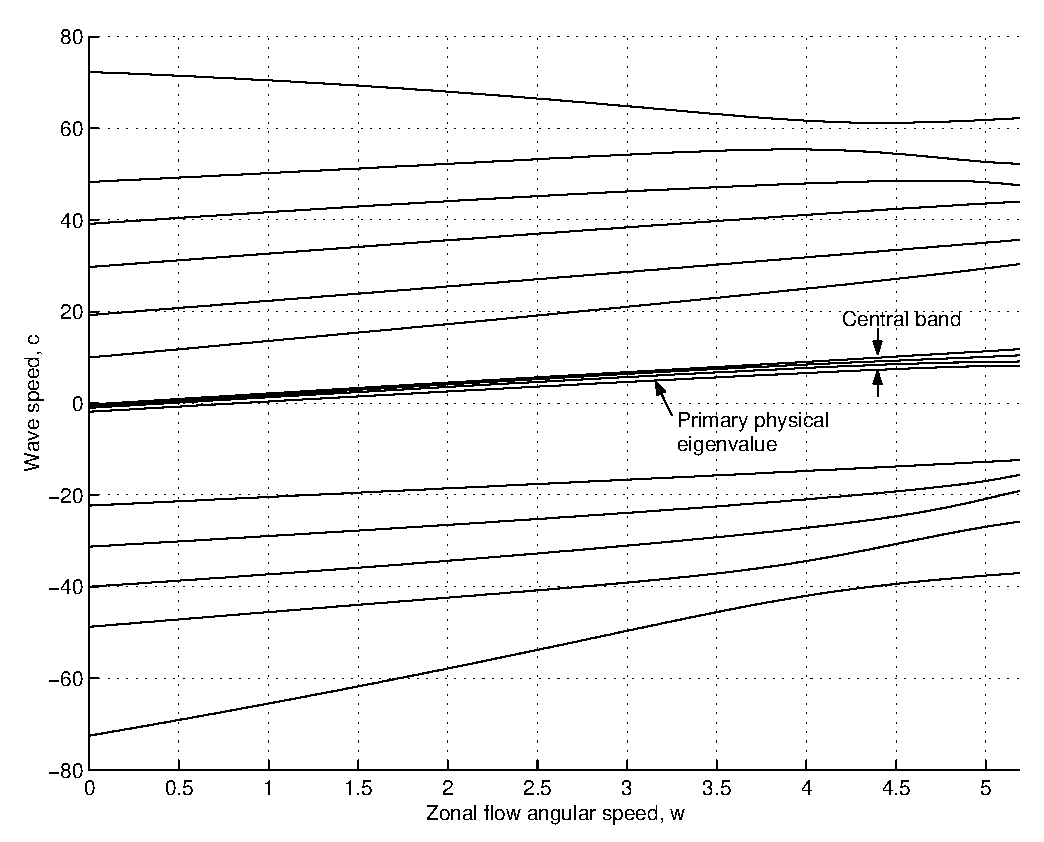
\includegraphics[scale=0.7]{IMAGES/kappa4fullspectrumN5.eps}
	\caption{Full eigen-spectrum for $\kappa=4$ with $N=5$.}
	\label{fig:wvcincompfull}
\end{figure}

It is evident that solutions to this problem can be classified into two groups: Those in the indicated central band in Figure~\ref{fig:wvcincompfull} and those lying outside this banded region. For the latter type, there was the initial suspicion that these were truncation induced solutions only; however further investigation at larger truncation levels revealed their persistence and convergence. The particular eigenvalues associated with these solutions are meaningless in a physical interpretation sense and thus can only be regarded as mathematically valid curiosities of the system. This is because the large values for the wavespeed that these solutions would imply are outside normally observed values on Earth. In addition the solutions themselves have an unphysical almost wave-less form with very little wave activity in the mid-latitudes and increased activity at the poles.
 
The \index{eigenvalues!central band}central band, on the other hand, contains much more realistic and physically meaningful solutions that demand further investigation. As labelled in Figure~\ref{fig:wvcincompfull}, we regard the banded region as consisting of a \index{eigenvalue!primary physical}primary physical eigenvalue and a series of harmonics above this base state. The primary physical eigenvalue is so labelled since it is the main solution of the system and corresponds to Rossby waves in the sense of a well defined wave structure and wavespeed.

As the truncation level is increased it is observed that this central banded region becomes more heavily populated, with higher order solutions converging to an upper limit as indicated in Figure~\ref{fig:wvcincompzoom}. While this behaviour is interesting in its own right, it is of little concern to us since the wavespeeds associated with such solutions are again rather too large to be considered as valid physical possibilities with reference to the Earth's atmosphere, where such speeds are never observed. We therefore restrict the rest of the discussion to an analysis of the primary physical eigenvalue and its main defining properties. 
\begin{figure}[htbp]
\psfrag{Zonal flow angular speed, w}{\scriptsize Zonal flow angular speed, $\omega$}
\psfrag{Wave speed, c}{\scriptsize Wavespeed, $c$}
%\psfrag{R-H solutions}{\scriptsize R-H solutions}
	\centering
		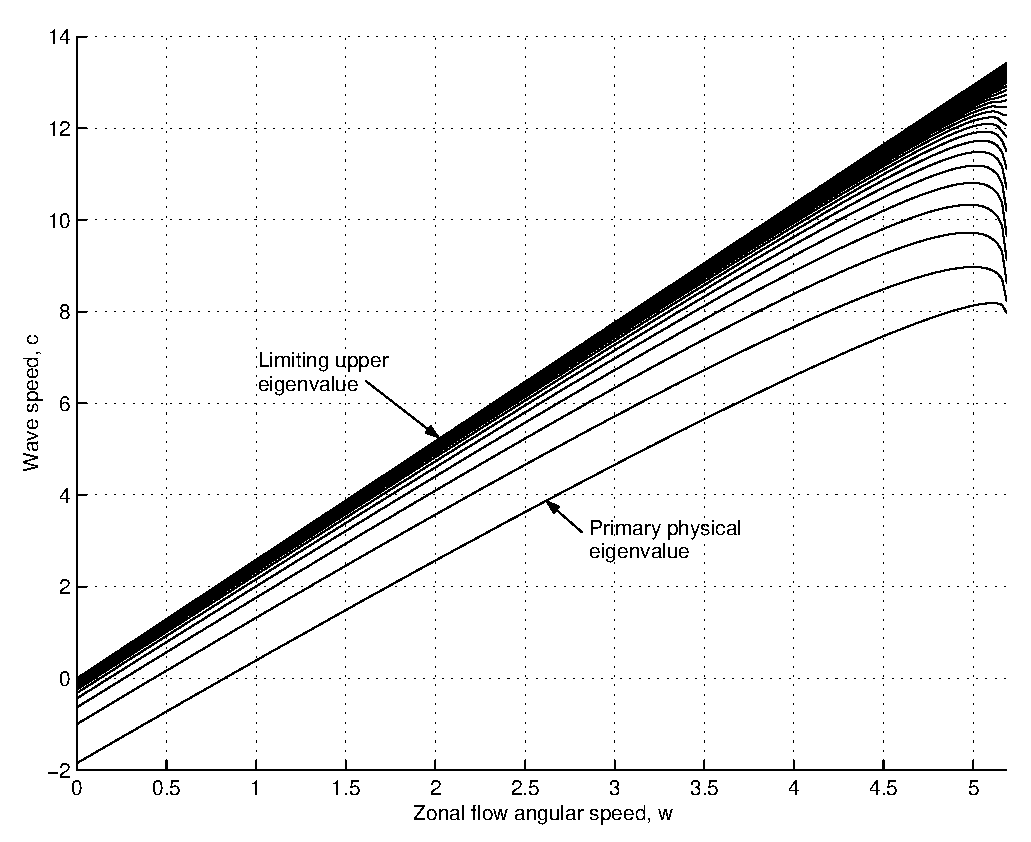
\includegraphics[scale=0.7]{IMAGES/kappa4zoomspectrumN50.eps}
	\caption{Zoomed eigen-spectrum for $\kappa=4$ with $N=50$.}
	\label{fig:wvcincompzoom}
\end{figure}

There are three main points to be made concerning Figure~\ref{fig:wvcincompzoom}. First and foremost we note that for values of $\omega$ away from the end points the wavespeed and $\omega$ relationship is close to linear. Secondly, there is a value of $\omega$ for which $c=0$ so that the linearized Rossby wave structure remains \index{Rossby wave!stationary}stationary relative to the Earth's surface. For values of $\omega$ below this critical value we have wave motion towards the west whereas for values higher we have eastward wave motion, allowing for a wide variety of atmospheric configurations. The final point concerns the behaviour at the upper end of the graph, in which no real confidence can be placed. The bending over of the solutions for large values of $\omega$ is a consequence of the fact that the height at the poles, $h_o$, is changing to conserve the total volume as previously discussed. At the other end of the graph, when $\omega=0$, we observe that the linearized solution predicts that waves with non-zero wavespeed are possible when there is no zonal flow structure. One way to interpret this behaviour is through the idea that the perturbations themselves are valid solutions of the system and that no zonal flow is required for them to exist; this idea is expanded by Pedlosky~\cite[pages 108--110]{Pedlosky:GFD}. Nonetheless, the solutions associated with values of $\omega$ away from the end points are physically reasonable, relevant and consistent with the Rossby-Haurwitz solutions, to be discussed in the next section.

\subsection{Comparison with Rossby-Haurwitz solution}
\label{subsec:rhandlincomp}
To provide evidence supporting the accuracy of the linearized solutions computed, it is useful to make a comparison between these solutions and the equivalent corresponding Rossby--Haurwitz solutions. To do this we make use of the wavespeed formula as presented in Haurwitz's classic paper \cite{Haurwitz:MAD} and later adopted by Williamson et al. in their test set. The particular formula is given by\index{Rossby--Haurwitz!formula}
\begin{equation}
c=\frac{\kappa(3+\kappa)\omega-2\Omega}{(1+\kappa)(2+\kappa)}
\end{equation}
which has been rewritten to reflect the naming conventions and variable names used in this work. Note that this equation clearly shows a linear relationship between $c$ and $\omega$. Also, Haurwitz's work does not allow one to fix the volume for the calculation, since it does not use a free-surface formulation, so we should expect some divergence from our solutions, which do take this into account.
\begin{figure}[htbp]
\psfrag{kappa=3}{\scriptsize $\kappa=3$}
\psfrag{kappa=4}{\scriptsize $\kappa=4$}
\psfrag{kappa=5}{\scriptsize $\kappa=5$}
\psfrag{Zonal flow angular speed, w}{\scriptsize Zonal flow angular speed, $\omega$}
\psfrag{Wave speed, c}{\scriptsize Wavespeed, $c$}
%\psfrag{R-H solutions}{\scriptsize R-H solutions}
	\centering
		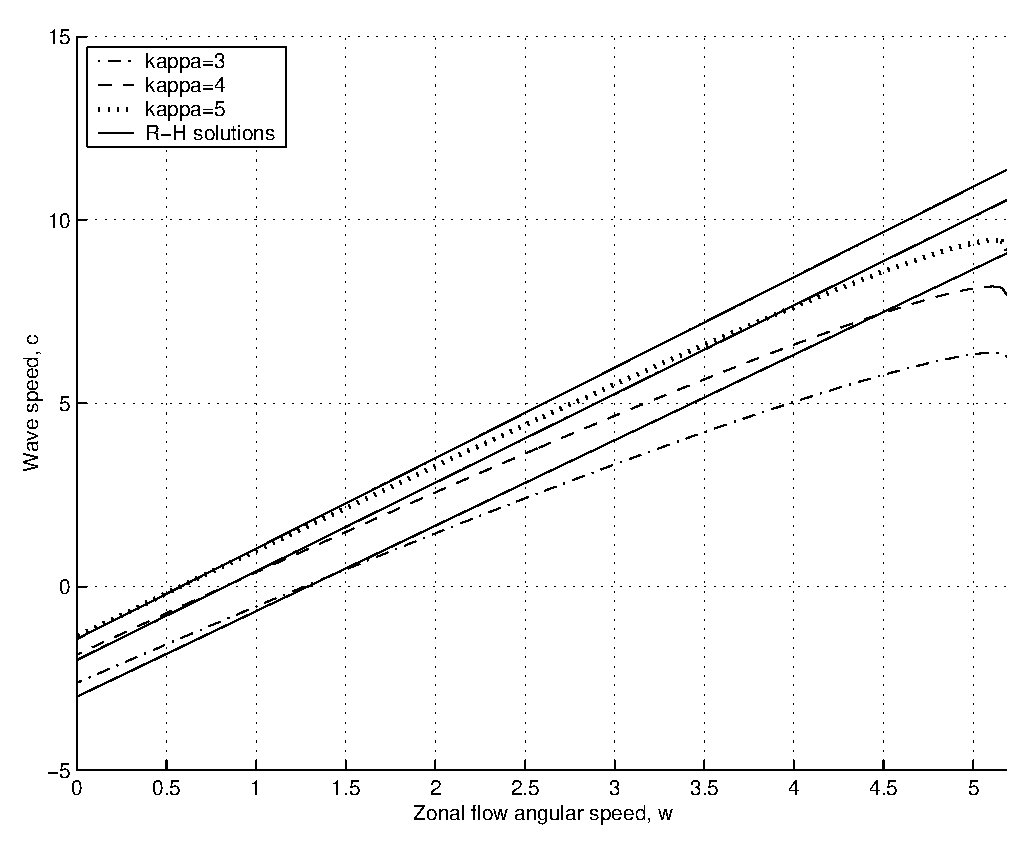
\includegraphics[scale=0.7]{IMAGES/wvchconst1.eps}
	\caption{Comparison of incompressible linearized and Rossby-Haurwitz solutions for $\kappa=3,4$ and 5 with $N=100$.}
	\label{fig:wvcincomp}
\end{figure}

To compare the two solution types we consider the primary physical eigenvalues for $\kappa=3,4$ and 5 with the equivalent Rossby-Haurwitz solutions over our valid $\omega$ range. Figure~\ref{fig:wvcincomp} shows the results of this comparison with the solid lines representing the equivalent \index{Rossby--Haurwitz!comparison with incompressible\\linearized solution}Rossby-Haurwitz solution for $\kappa=3$ to 5 from bottom to top respectively. In general one can conclude that the two models have good agreement, especially so for values of $\omega$ in the range $0<\omega<2$ where the effect of the volume matching is minimal. In fact better agreement is observed if one does not take the volume matching into consideration and fixes $h_o=1$, however the validity of the comparison between various values of $\omega$ is questionable in this case.

It is also useful to examine the resulting free-surface contours produced by both models. In order to match the height contour levels it it necessary to specify some equivalent value of the wave amplitude $\epsilon$. To make comparison possible we choose to match the two \index{height field matching}height fields at $(\eta,\phi)=(0,\pi/4)$ which represents a reasonable mid point level in each contour set. It is interesting to note that despite the fact that Haurwitz did not use a free-surface formulation, the resulting height field may be calculated via an analysis of the pressure field, as developed by Phillips\cite{Phillips:NIP}.

\begin{figure}[htbp]
	\centering
		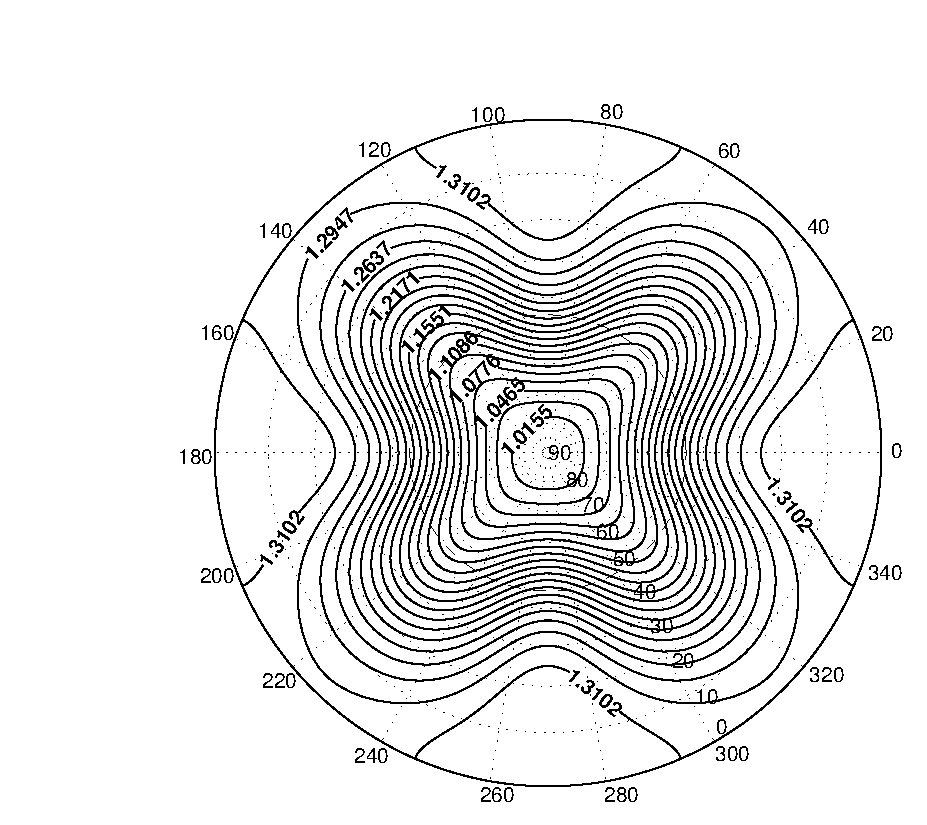
\includegraphics[scale=0.75]{IMAGES/swfsconts.eps}
	\caption{Incompresible shallow atmosphere free-surface contours for $\kappa=4$ with $N=100$.}
	\label{fig:swfsconts}
\end{figure}
\begin{figure}[htbp]
	\centering
		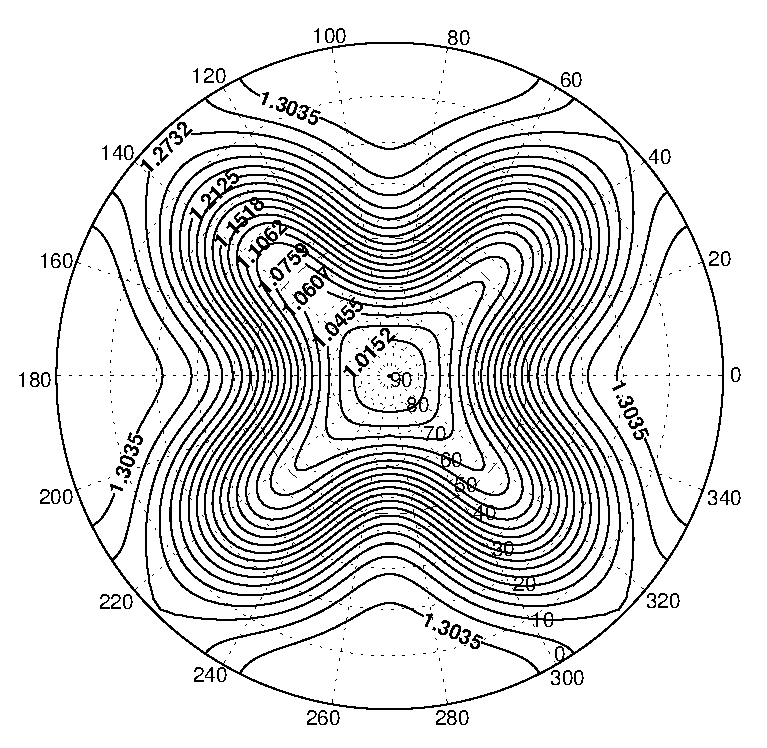
\includegraphics[scale=0.75]{IMAGES/rhfsconts.eps}
	\caption{Rossby--Haurwitz \index{Rossby--Haurwitz!free-surface contours}free-surface contours for $\kappa=4$.}
	\label{fig:rhfsconts}
\end{figure}

Figures \ref{fig:swfsconts} and \ref{fig:rhfsconts} provide a solution comparison both qualitatively, through a visual comparison, and quantitatively, through the specific contour levels of each height field. The latitudinal circle at $\phi=\pi/4$ is indicated to show where the match takes place. All plots were made using a \index{polar stereographic projection}polar stereographic projection of the Northern Hemisphere, described exhaustively in Snyder's monumental work\cite{Snyder:MP}. Of particular interest is the slight pinching of crests and troughs for the Rossby--Haurwitz wave structure that is not evident in the linearized solution. This in turn forces the lower heights, and hence pressures, near the poles to extend further towards the equator in the Rossby--Haurwitz solution. However, overall there is very close agreement between both types of solutions, encouraging one to assume that these indeed are valid approximate solutions of the full non-linear governing equations.

As a final supporting statement we investigate the nature of the corresponding velocity vector field for the free-surface presented in Figure~\ref{fig:swfsconts}. From a \index{geostrophic approximation}geostrophic point of view we would expect the fluid streamlines to be nearly parallel to the pressure contours, something which is observed in Figure~\ref{fig:fsvelfield}. Additionally we have increasingly diminishing flow as we approach either pole, which converges to the required stagnation point when $\phi=\pm \pi/2$. Since the particular viewpoint of the projection means that the sphere's rotation is counter clockwise when viewed from above, we see that fluid flow is directed in the same direction as the underlying zonal flow with the Rossby wave pattern moving relative to this mean fluid progression.
\begin{figure}[htbp]
	\centering
		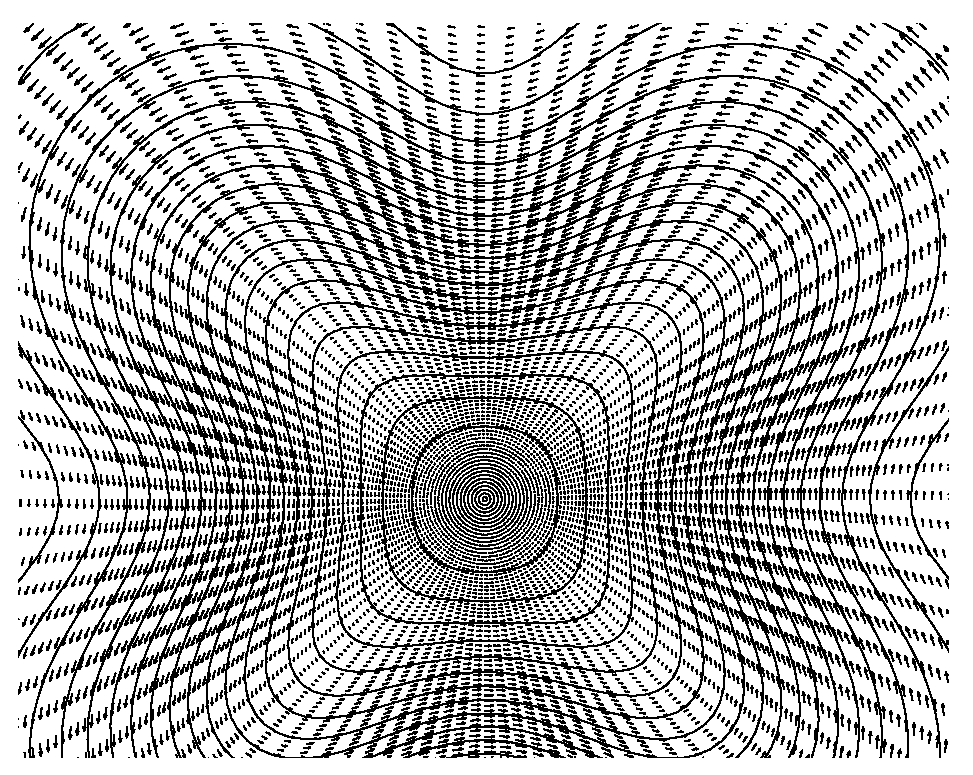
\includegraphics[scale=0.8]{IMAGES/fsvelfield.eps}
	\caption{Incompressible shallow atmosphere free-surface contours with corresponding velocity vector field for $\kappa=4$ with $N=100$}
	\label{fig:fsvelfield}
\end{figure}

In this chapter we have explored linearized solutions of the incompressible, non-dimensional shallow atmosphere equations. The solutions that were obtained for particular values of longitudinal wave number $\kappa$ were found to be in close agreement with the corresponding Rossby-Haurwitz solutions. Not only do the linearized solutions provide helpful insight into this complex dynamical system, they can also be used as a base starting point for a more thorough investigation of the complete nonlinear system. This problem is addressed in the next chapter.


% chap3.tex (Chapter 3 of the thesis)

\chapter[ANOTHER CHAPTER]{Another Chapter}

\section{New Section}
More stuff here too...

% chap4.tex (Chapter 4 of the thesis)

\chapter[COMPRESSIBLE LINEARIZED SHALLOW ATMOSPHERE\\ MODEL]{COMPRESSIBLE LINEARIZED SHALLOW ATMOSPHERE\\ MODEL}
\label{chap:4}
\section{Derivation}
We consider here the derivation of the \index{shallow atmosphere!compressible}compressible shallow atmosphere equations in a rotating spherical coordinate system, again following the general approach developed in Pedlosky\cite{Pedlosky:GFD}, with appropriate modifications for a compressible fluid. For ease of reference and completeness we treat the derivation in this section as distinct from that of the incompressible case derived in Section~\ref{sec:incompderiv}, although both derivations share some similarities.
\begin{figure}[htbp]
\psfrag{hd}{\large $h$}
\psfrag{hb}{\large $h_b$}
\psfrag{h}{\large $\bar{h}$}
\psfrag{r=a}{\large $r=a$}
	\centering
		\includegraphics[scale=0.65]{IMAGES/freesurfparams.eps}
	\caption{Free-surface height parameters}
	\label{fig:freesurfparams1}
\end{figure}

Refering to Figure~\ref{fig:freesurfparams1}, define \index{$\bar{h}$, free-surface height}$\bar{h}$ as the radial height above the level surface $r=a$ of a free-surface surrounding a rotating reference sphere of radius $r=a$.  Additionally, define \index{$h$, free-surface depth}$h$ and $h_b$ as the depth of the fluid and the height of the underlying mountains respectively. The height of the free-surface, $\bar{h}$, can be given in terms of the two parameters $h_b$ and $h$ as
\begin{equation}
	\bar{h}=h_b+h.
\end{equation}
Although the generality of this setup affords the representation of a much wider class of problem we will restrict ourselves to the case when there is no underlying mountain specification so that $h_b=0$, leading to
\begin{equation}
	\bar{h}=h. \label{eq:hequalhbar}
\end{equation}

For this study we will be concerned with compressible, \index{adiabatic flow}adiabatic fluid flow. Because the fluid is adiabatic the rate of heat addition, $q_h$ in \eqref{eq:energy1}, will be zero. Additionally, due to the nature of the spherical coordinate system the vertical coordinate $r$ appears explicitly in the dynamical equations; however, we can adequately approximate this by $r=a$, see Holton~\cite{Holton:IDM}. Adopting the above approximations, we obtain the following modified form for the compressible dynamical equations, \eqref{eq:scfmass}--\eqref{eq:gaslaw}, presented in Chapter~\ref{chap:1}.

{\bfseries Mass}
\begin{equation}
\drhod{t}+\frac{1}{a\cos\phi}\left[ \frac{\partial}{\partial r}(a\ur\rho\cos\phi) + \frac{\partial}{\partial \lambda}(\ulam\rho) + \frac{\partial}{\partial \phi}(\uphi\rho\cos\phi)  \right]=0, \label{eq:compmass}
\end{equation}
{\bfseries \boldmath$r$ momentum}
\begin{equation}
\durd{t} +\ur\durd{r}+ \frac{\ulam}{a\cos\phi}\durd{\lambda}+\frac{\uphi}{a}\durd{\phi}-\frac{\ulams+\uphis}{a}-2\Omega\ulam\cos\phi+\frac{1}{\rho}\dpd{r}= -g,\label{eq:compr}
\end{equation}
{\bfseries \boldmath$\lambda$ momentum}
\begin{multline}
\dulamd{t} +\ur\dulamd{r}+ \frac{\ulam}{a\cos\phi}\dulamd{\lambda}+\frac{\uphi}{a}\dulamd{\phi}+\frac{\ur\ulam-\ulam\uphi\tan\phi}{a}\\+2\Omega(\ur\cos\phi-\uphi\sin\phi)+\frac{1}{a\rho\cos\phi}\dpd{\lambda}= 0, \label{eq:complam}
\end{multline}
{\bfseries \boldmath$\phi$ momentum}
\begin{multline}
\duphid{t} +\ur\duphid{r}+ \frac{\ulam}{a\cos\phi}\duphid{\lambda}+\frac{\uphi}{a}\duphid{\phi}+\frac{\ur\uphi+\ulams\tan\phi}{a}\\+2\Omega\ulam\sin\phi+\frac{1}{a\rho}\dpd{\phi}= 0, \label{eq:compphi}
\end{multline}
{\bfseries Energy}
\begin{equation}
\rho c_v \frac{\mbox{D} T}{\mbox{D} t} - \frac{p}{\rho}\frac{\mbox{D} \rho}{\mbox{D} t}=0,
\label{eq:compenergy}
\end{equation}
{\bfseries Gas Law}
\begin{equation}
p=\rho R T.
\label{eq:compgaslaw}
\end{equation}
Using the gas law, \eqref{eq:compgaslaw}, we can write the energy equation, (\ref{eq:compenergy}), as
\begin{equation}
\frac{1}{(\gamma-1)T}\frac{\mbox{D} T}{\mbox{D} t}-\frac{1}{\rho}\frac{\mbox{D} \rho}{\mbox{D} t}=0,
\label{eq:compenergy1}
\end{equation}
where we have used the thermodynamic relationship $c_v/R=1/(\gamma-1)$. The absence of heat addition makes it possible to integrate the total derivatives in \eqref{eq:compenergy1},
\begin{equation*}
\int \frac{\mbox{D}T}{T}=\int (\gamma-1) \frac{\mbox{D}\rho}{\rho} + \mbox{constant},
\end{equation*}
to give
\begin{equation}
T(\rho)=A\rho^{\gamma-1}, \label{eq:Tinrho}
\end{equation}
where $A$ is a constant of integration whose value is determined for each specific atmospheric composition. From (\ref{eq:Tinrho}) and (\ref{eq:compgaslaw}) it is immediately obvious that the pressure can also be expressed as a function of density of the form
\begin{equation}
p(\rho)=\beta\rho^{\gamma}, \label{eq:pinrho}
\end{equation}
where we have defined the constant $\beta=A \,R$. Thermodynamically, equation \eqref{eq:pinrho} indicates that the atmosphere model is \index{polytropic atmosphere}polytropic.

The underlying assumption of the \index{shallow atmosphere approximation}shallow atmosphere approximation is that motion mainly occurs on level radial surfaces of the spherical coordinate system and less so in the $r$ direction, effectively confining the velocity to motion that is predominantly tangent to the surface of the sphere. Mathematically we can write this statement as
\begin{align}
\ur &\approx O(\epsilon), \label{eq:urapproxcom}\\
\ulam &\approx O(1), \\
\uphi &\approx O(1), \label{eq:uphiapproxcom}
\end{align}
where $\epsilon$ is a small parameter that reflects the shallowness of the atmosphere relative to the radius of the sphere. Consider now the implications of this approximation for the $r$ momentum equation \eqref{eq:compr}. We argue that the total derivative terms $\durd{t}$, $\ur\durd{r}$, $\frac{\ulam}{a\cos\phi}\durd{\lambda}$ and $\frac{\uphi}{a}\durd{\phi}$ are all $O(\epsilon)$ so that the $r$ momentum equation reduces to 
\begin{equation}
-\frac{\ulams+\uphis}{a}-2\Omega\ulam\cos\phi+\frac{1}{\rho}\dpd{r}= -g. \label{eq:compr1}
\end{equation}
Additionally, we assume that \eqref{eq:compr1} is dominated by \index{hydrostatic approximation}hydrostatics\footnote{We can be more rigorous than this and use a scale analysis approach to argue this point. See Pedlosky\cite[page 60]{Pedlosky:GFD} for the finer details of this process} so that effectively we have
\begin{equation}
\dpd{r}= -\rho g ,\label{eq:compr2}
\end{equation}
which in conjunction with \eqref{eq:pinrho}, we arrive at
\begin{equation*}
\rho^{\gamma-2}\drhod{r} = \frac{-g}{\beta \gamma}.
\end{equation*}
Integration with respect to $r$ yields
\begin{equation*}
\rho^{\gamma-1}(r,\lambda,\phi,t)= f_1(\lambda,\phi,t)-\frac{g(\gamma-1)r}{\beta \gamma}.
\end{equation*}

The value of $f_1(\lambda,\phi,t)$ is ascertained by assuming that on the free-surface,  $r=a+\bar{h}(\lambda,\phi,t)$, the density has the constant value $\rhoo$, so that
\begin{equation}
\rho^{\gamma-1}(r,\lambda,\phi,t)=\rho^{\gamma-1}_{\scriptscriptstyle 0}+\frac{g(\gamma-1)}{\beta \gamma} (a+\bar{h}(\lambda,\phi,t)-r). \label{eq:comprhobasic}
\end{equation}
Using \eqref{eq:comprhobasic} we can solve for $\rho$. With the addition of \eqref{eq:Tinrho} and \eqref{eq:pinrho} we obtain formulae for the thermodynamic variables in the problem. The results are
\begin{align}
\rho(r,\lambda,\phi,t) &=\left[\rho^{\gamma-1}_{\scriptscriptstyle 0}+\frac{g(\gamma-1)}{\beta \gamma} (a+\bar{h}(\lambda,\phi,t)-r) \right]^{\frac{1}{\gamma-1}}, \label{eq:comprho}\\
p(r,\lambda,\phi,t) &= \beta\left[\rho^{\gamma-1}_{\scriptscriptstyle 0}+\frac{g(\gamma-1)}{\beta \gamma} (a+\bar{h}(\lambda,\phi,t)-r) \right]^{\frac{\gamma}{\gamma-1}}, \label{eq:compp}\\
T(r,\lambda,\phi,t) &= A\left[\rho^{\gamma-1}_{\scriptscriptstyle 0}+\frac{g(\gamma-1)}{\beta \gamma} (a+\bar{h}(\lambda,\phi,t)-r) \right] .\label{eq:compT}
\end{align}

From \eqref{eq:comprho} and \eqref{eq:compp} we can show that
\begin{align}
\dpd{\lambda}&=g \rho \dhd{\lambda},\\
\dpd{\phi}&=g \rho \dhd{\phi},
\end{align}
so that the pressure gradient terms in the $\lambda$ and $\phi$ momentum equations, \eqref{eq:complam} and \eqref{eq:compphi}, are given by
\begin{align}
\frac{1}{\rho} \dpd{\lambda}&=g \dhd{\lambda},\label{eq:compdpdl}\\
\frac{1}{\rho} \dpd{\phi}&=g \dhd{\phi}. \label{eq:compdpdp}
\end{align}

Equations \eqref{eq:compdpdl} and \eqref{eq:compdpdp} imply that the \index{horizontal!pressure gradient}horizontal pressure gradient terms are $r$-independent, which in turn implies that all \index{horizontal!acceleration}accelerations in \eqref{eq:complam} and \eqref{eq:compphi} must also be $r$-independent. Thus the individual velocity components are $r$-independent if they are initially so, see \cite{Pedlosky:GFD}, leading to
\begin{align}
\ulam &\equiv \ulam(\lambda,\phi,t), \label{eq:ulamnor}\\
\uphi &\equiv \uphi(\lambda,\phi,t). \label{eq:uphinor}
\end{align}

Using the shallow atmosphere approximation contained in \eqref{eq:urapproxcom}--\eqref{eq:uphiapproxcom}, the two remaining momentum equations, \eqref{eq:complam} and \eqref{eq:compphi}, become

{\bfseries $\lambda$ momentum}
\begin{equation}
\dulamd{t} + \frac{\ulam}{a\cos\phi}\dulamd{\lambda}+\frac{\uphi}{a}\dulamd{\phi}-\frac{\ulam\uphi\tan\phi}{a}-2\Omega\uphi\sin\phi+\frac{g}{a\cos\phi}\dhd{\lambda}= 0, \label{eq:complam1}
\end{equation}
{\bfseries $\phi$ momentum}
\begin{equation}
\duphid{t}+ \frac{\ulam}{a\cos\phi}\duphid{\lambda}+\frac{\uphi}{a}\duphid{\phi}+\frac{\ulams\tan\phi}{a}+2\Omega\ulam\sin\phi+\frac{g}{a}\dhd{\phi}= 0. \label{eq:compphi1}
\end{equation}

We now consider the task of integrating the mass equation, \eqref{eq:compmass}, with respect to the radial coordinate $r$. We introduce the function
\begin{equation}
\rhoI=\int \rho (r,\lambda,\phi,t)\,dr \label{eq:rhoint}
\end{equation}
so that
\begin{equation}
\rho = \frac{\partial \rhoI}{\partial r}.
\end{equation}
The definition of $\rhoI$, in combination with \eqref{eq:ulamnor} and \eqref{eq:uphinor}, enables the mass equation to be written as
\begin{equation}
\frac{\partial}{\partial r} \left[ \drhoId{t} + \frac{1}{a\cos\phi}\left(a\ur\cos\phi \drhoId{r} + \frac{\partial}{\partial \lambda}\left(\ulam \rhoI \right) + \frac{\partial}{\partial \phi}\left(\uphi \rhoI \cos\phi\right) \right) \right]=0, \label{eq:compmassmod}
\end{equation}
which can be integrated with respect to $r$ and manipulated to give
\begin{equation}
\ur \rho + \drhoId{t} + \frac{1}{a\cos\phi}\frac{\partial}{\partial \lambda}\left(\ulam \rhoI \right)+\frac{1}{a\cos\phi}\frac{\partial}{\partial \phi}\left(\uphi \rhoI \cos\phi\right)=f_2(\lambda,\phi,t). \label{eq:compmassint}
\end{equation}
To determine $f_2(\lambda,\phi,t)$ we note that on the lower boundary we must have no normal flow, otherwise the fluid would penetrate the surface and breach the conservation of mass requirement. Thus on $r=a+h_b(\lambda,\phi)$ we must enforce the condition $\bol{q}\cdot\bol{n}=0$ where $\bol{n}$ is a normal to the surface. We can easily show that the normal to the lower boundary is given by
\begin{equation}
\bol{n}=\mbox{\bfseries e}_{r}-\frac{1}{a\cos\phi}\dhbd{\lambda}\mbox{\bfseries e}_{\lambda}-\frac{1}{a}\dhbd{\phi}\mbox{\bfseries e}_{\phi},
\end{equation}
so that
\begin{equation}
\bol{q}\cdot\bol{n}=\ur(a+h_b,\lambda,\phi,t)-\frac{\ulam}{a\cos\phi}\dhbd{\lambda}-\frac{\uphi}{a}\dhbd{\phi}=0.
\end{equation}
Solving for $\ur$ we obtain
\begin{equation}
\ur(a+h_b,\lambda,\phi,t)=\frac{\ulam}{a\cos\phi}\dhbd{\lambda}+\frac{\uphi}{a}\dhbd{\phi}. \label{eq:compurhb}
\end{equation}
Substituting \eqref{eq:compurhb} into \eqref{eq:compmassint} and evaluating at $r=a+h_b$ allows us to solve for $f_2(\lambda,\phi,t)$, which we in turn substitute back into \eqref{eq:compmassint}. After simplification we obtain
\begin{align}
\ur \rho + \drhoId{t} &+ \frac{1}{a\cos\phi}\frac{\partial}{\partial \lambda}\left(\ulam \rhoI \right)+\frac{1}{a\cos\phi}\frac{\partial}{\partial \phi}\left(\uphi \rhoI \cos\phi\right)- \left.\drhoId{t}\right|_{a+h_b} \notag\\
&-\rho|_{a+h_b}\left[ \frac{\ulam}{a\cos\phi}\dhbd{\lambda} + \frac{\uphi}{a}\dhbd{\phi} \right]  - \frac{1}{a\cos\phi}\left.\frac{\partial}{\partial \lambda}\left(\ulam \rhoI \right)\right|_{a+h_b} \notag\\&- \frac{1}{a\cos\phi}\left.\frac{\partial}{\partial \phi}\left(\uphi \rhoI \cos\phi \right)\right|_{a+h_b} = 0 \label{eq:urgen1comp}
\end{align}
where $\rho|_{a+h_b}$ is taken to mean $\rho$ evaluated at $r=a+h_b$, similarly for $\rhoI$ and its derivatives.

On the upper boundary we enforce the \index{kinematic condition}kinematic condition 
\begin{equation*}
\frac{\mbox{\footnotesize D\ }}{\mbox{\footnotesize D}t}\left[r-a-\bar{h}(\lambda,\phi,t)\right]=0,
\end{equation*} which states that the fluid can not penetrate the free-surface. Expanding the total derivative and solving for $\ur$ gives
\begin{equation}
\ur(a+\bar{h},\lambda,\phi,t)=\dhd{t}+\frac{\ulam}{a\cos\phi}\dhd{\lambda}+\frac{\uphi}{a}\dhd{\phi}.
\label{eq:urfscomp}
\end{equation}
Finally, substitution of \eqref{eq:urfscomp} into \eqref{eq:urgen1comp} and subsequent simplification yields the incompressible shallow atmosphere mass equation given by
\begin{align}
&\Biggl[\rho|_{a+\bar{h}} \dhd{t} + \left.\drhoId{t}\right|_{a+\bar{h}} - \left.\drhoId{t}\right|_{a+h_b}\Biggr]+\Biggl[\frac{\ulam \rho|_{a+\bar{h}}}{a\cos\phi}\dhd{\lambda} +\frac{1}{a\cos\phi}\left.\frac{\partial}{\partial \lambda}\left(\ulam \rhoI \right)\right|_{a+\bar{h}} \notag \\
& \qquad - \frac{\ulam \rho|_{a+h_b}}{a\cos\phi}\dhbd{\lambda} -\frac{1}{a\cos\phi}\left.\frac{\partial}{\partial \lambda}\left(\ulam \rhoI \right)\right|_{a+h_b} \Biggr] + \Biggl[\frac{\uphi \rho|_{a+\bar{h}}}{a}\dhd{\phi} \notag \\
& \qquad +\frac{1}{a\cos\phi}\left.\frac{\partial}{\partial \phi}\left(\uphi \rhoI \cos\phi \right)\right|_{a+\bar{h}} - \frac{\uphi \rho|_{a+h_b}}{a}\dhbd{\phi} \notag \\&\qquad -\frac{1}{a\cos\phi}\left.\frac{\partial}{\partial \phi}\left(\uphi \rhoI \cos\phi\right)\right|_{a+h_b} \Biggr] = 0. \label{eq:compmassunsimp}
\end{align}

Equation \eqref{eq:compmassunsimp} can be simplified considerably by noting that the derivatives of $\rhoI$ can be expressed in terms of the density, $\rho$, and the free-surface, $\bar{h}$. Substitution of \eqref{eq:comprho} into \eqref{eq:rhoint} and subsequent evaluation of the integral yields
\begin{align}
\rhoI(r,\lambda,\phi,t)&=-\frac{\beta}{g}\left[\rho^{\gamma-1}_{\scriptscriptstyle 0}+\frac{g(\gamma-1)}{\beta \gamma} (a+\bar{h}(\lambda,\phi,t)-r) \right]^{\frac{\gamma}{\gamma-1}}+c_0 \label{eq:rhoIeval1} \\
&=-\frac{1}{g}p(r,\lambda,\phi,t)+c_0, \label{eq:rhoIeval2}
\end{align}
for constant of integration $c_0$. We now use \eqref{eq:rhoIeval1} to calculate derivatives of $\rhoI$ with respect to $\lambda$, $\phi$ and $t$. It is straightforward to show that
\begin{equation*}
\drhoId{t}=-\rho \dhd{t}, \qquad \drhoId{\lambda}=-\rho \dhd{\lambda}, \qquad \drhoId{\phi}=-\rho \dhd{\phi},
\end{equation*} 
and these expressions may now be used to simplify the mass equation so that algebraic manipulation of \eqref{eq:compmassunsimp} leads to
\begin{multline}
\rho|_{a+h_b}\dhd{t}+\frac{1}{a\cos\phi}\left(\rhoI|_{a+\bar{h}}-\rhoI|_{a+h_b} \right)\left[ \dulamd{\lambda} + \frac{\partial}{\partial \phi}\left(\uphi \cos\phi \right) \right] \\
+\frac{\rho|_{a+h_b}}{a\cos\phi}\left[\ulam \left(\dhd{\lambda}-\dhbd{\lambda} \right)+\uphi\cos\phi\left(\dhd{\phi}-\dhbd{\phi} \right) \right]=0 \label{eq:compmasssimp}
\end{multline}

In this study we are only concerned with the special case of bottom topography in which $h_b=0$. Thus, from equation \eqref{eq:hequalhbar}, we have equality of the depth of the atmosphere, $h$, and the free-surface height, $\bar{h}$, allowing us to drop the overbar ($\bar{\ }$) notation and simplify further to give
\begin{multline}
\rho|_{a}\dhdd{t}+\frac{1}{a\cos\phi}\left(\rhoI|_{a+h}-\rhoI|_{a} \right)\left[ \dulamd{\lambda} + \frac{\partial}{\partial \phi}\left(\uphi \cos\phi \right) \right] \\
+\frac{\rho|_{a}}{a\cos\phi}\left[\ulam\dhdd{\lambda}+\uphi\cos\phi \dhdd{\phi}\right]=0. \label{eq:compmasssimpfur}
\end{multline}

Note that from \eqref{eq:rhoIeval2} we can replace all occurances of $\rhoI$ with equivalent pressure terms so that we can also write \eqref{eq:compmasssimpfur} as
\begin{equation}
\rho|_{a}\dhdd{t}+\frac{1}{a\cos\phi}\left[\frac{\partial}{\partial \lambda} \left(\frac{\ulam}{g}\left( p|_a-p|_{a+h}\right) \right) +\frac{\partial}{\partial \phi} \left(\frac{\uphi\cos\phi}{g}\left( p|_a-p|_{a+h}\right) \right)\right] =0. \label{eq:compmasssimppress}
\end{equation}
As a check of the validity of this equation we note that if the fluid is incompressible, that is $\rho$ is constant, then $p=p_0+\rho g (a+h-r)$ so that
\begin{equation*}
p|_a-p|_{a+h}=\rho g h,
\end{equation*}
and thus \eqref{eq:compmasssimppress} becomes
\begin{equation*}
\dhdd{t}+\frac{1}{a\cos\phi}\left[\frac{\partial}{\partial \lambda} \left(\ulam h \right) +\frac{\partial}{\partial \phi} \left(\uphi h \cos\phi \right)\right] =0,
\end{equation*}
which is identical to \eqref{eq:massincom} from the incompressible derivation.

To the extent that the aim of this study is to investigate progressive Rossby wave structures, we again introduce a coordinate frame involving the progressive angular wavespeed $c$ and longitudinal and time coordinates, $\lambda$ and $t$, as in Section~\ref{sec:progresswave} of Chapter~\ref{chap:2}. We define
\begin{equation*}
\eta=\lambda-c t
\end{equation*}
as the new travelling coordinate system, with the effect of the $-ct$ term being to translate any initial wave structure either towards the west ($c<0$) or towards the east ($c>0$) with constant angular speed $c$. 

Applying the coordinate transformation to the governing equations and writing $f=2\Omega\sin\phi$, we can express the complete \index{conservation equations!dimensional compressible}dimensional dynamical equations of motion for a thin layer of compressible fluid with a free-surface in a rotating spherical coordinate system as 

{\bfseries mass}
\begin{equation}
-c g a \cos\phi \rho|_{a}\dhdd{\eta}+\left[\frac{\partial}{\partial \eta} \left(\ulam\left( p|_a-p|_{a+h}\right) \right) +\frac{\partial}{\partial \phi} \left(\uphi\cos\phi\left( p|_a-p|_{a+h}\right) \right)\right] =0, \label{eq:compmassp}
\end{equation}
{\bfseries \boldmath$\lambda$ momentum}
\begin{equation}
\left(\frac{\ulam}{a}-c\cos\phi\right)\dulamd{\eta} + \frac{\uphi\cos\phi}{a}\dulamd{\phi} - \left(f\cos\phi + \frac{\ulam}{a}\sin\phi \right)\uphi + \frac{g}{a}\dhdd{\eta} = 0, \label{eq:lamcomp}
\end{equation}
{\bfseries \boldmath$\phi$ momentum}
\begin{equation}
\left(\frac{\ulam}{a}-c\cos\phi\right)\duphid{\eta}+\frac{\uphi\cos\phi}{a}\duphid{\phi}+\left(f\cos\phi+\frac{\ulam}{a}\sin\phi \right)\ulam+\frac{g\cos\phi}{a}\dhdd{\phi}=0, \label{eq:phicomp}
\end{equation}
where the density and pressure are defined by
\begin{equation}
\rho(r,\eta,\phi) =\left[\rho^{\gamma-1}_{\scriptscriptstyle 0}+\frac{g(\gamma-1)}{\beta \gamma} (a+h(\eta,\phi)-r) \right]^{\frac{1}{\gamma-1}} \label{eq:dencomp}
\end{equation}
and
\begin{equation}
p(r,\eta,\phi) = \beta\left[\rho^{\gamma-1}_{\scriptscriptstyle 0}+\frac{g(\gamma-1)}{\beta \gamma} (a+h(\eta,\phi)-r) \right]^{\frac{\gamma}{\gamma-1}} \label{eq:pcomp}
\end{equation}
respectively.

\section{Non-dimensionalization and Problem Simplification}
\subsection{Non-dimensionalization}
We now consider the non-dimensionalization of the compressible shallow atmosphere equations. First we define the following characteristic values, for each reference scale contained in the problem, as
\begin{align*}
v_{\mbox{\tiny ref}} & \equiv \mbox{characteristic speed,}\\
h_{\mbox{\tiny ref}} & \equiv \mbox{characteristic free-surface height,} \\
c_{\mbox{\tiny ref}} & \equiv \mbox{characteristic angular speed,} \\
\rho_{\mbox{\tiny ref}} & \equiv \mbox{characteristic density,} \\
p_{\mbox{\tiny ref}} & \equiv \mbox{characteristic pressure.}
\end{align*}
Using these dimensional characteristic values we now rescale all the field variables to dimensionless form giving
\begin{align}
\hat{u}_{\scriptscriptstyle \lambda}=\frac{\ulam}{v_{\mbox{\tiny ref}}} \quad & \Rightarrow \quad \ulam = v_{\mbox{\tiny ref}} \hat{u}_{\scriptscriptstyle \lambda}, \label{eq:ulamhatcomp}\\
\hat{u}_{\scriptscriptstyle \phi}=\frac{\uphi}{v_{\mbox{\tiny ref}}} \quad & \Rightarrow \quad \ulam = v_{\mbox{\tiny ref}} \hat{u}_{\scriptscriptstyle \phi}, \label{eq:uphihatcomp}\\
\hat{h}=\frac{h}{h_{\mbox{\tiny ref}}} \quad & \Rightarrow \quad h = h_{\mbox{\tiny ref}} \hat{h}, \label{eq:hhatcomp}\\
\hat{c}=\frac{c}{c_{\mbox{\tiny ref}}} \quad & \Rightarrow \quad c = c_{\mbox{\tiny ref}} \hat{c}, \label{eq:chatcomp}\\
\hat{\rho}=\frac{\rho}{\rho_{\mbox{\tiny ref}}} \quad & \Rightarrow \quad \rho = \rho_{\mbox{\tiny ref}} \hat{\rho}, \label{eq:rhohatcomp}\\
\hat{p}=\frac{p}{p_{\mbox{\tiny ref}}} \quad & \Rightarrow \quad p = p_{\mbox{\tiny ref}} \hat{p}, \label{eq:phatcomp}
\end{align}
where the hat $\hat{}$ denotes a dimensionless variable. Substituting equations \eqref{eq:ulamhatcomp}--\eqref{eq:phatcomp} into \eqref{eq:compmassp}, \eqref{eq:lamcomp},  \eqref{eq:phicomp} and manipulating, we obtain

{\bfseries mass}
\begin{equation}
-\mathrm{Sr}\hat{c} \hat{\rho}|_{a} \cos\phi \frac{\partial \hat{h}}{\partial \eta}+\left( \frac{\mbox{Fr}}{\mbox{M}}\right)^2 \left[\frac{\partial}{\partial \eta} \left(\hat{u}_{\scriptscriptstyle \lambda}\left( \hat{p}|_a-\hat{p}|_{a+h}\right) \right) +\frac{\partial}{\partial \phi} \left(\hat{u}_{\scriptscriptstyle \phi}\cos\phi\left( \hat{p}|_a-\hat{p}|_{a+h}\right) \right)\right] =0, \label{eq:masscom2non}
\end{equation}
{\bfseries \boldmath$\lambda$ momentum}
\begin{equation}
\left(\hat{u}_{\scriptscriptstyle \lambda}-\mathrm{Sr}\,\hat{c}\cos\phi\right)\frac{\partial \hat{u}_{\scriptscriptstyle \lambda}}{\partial \eta} + \hat{u}_{\scriptscriptstyle \phi}\cos\phi\frac{\partial \, \hat{u}_{\scriptscriptstyle \lambda}}{\partial \, \phi} - \left(\frac{\cos\phi}{\mathrm{Ro}} + \hat{u}_{\scriptscriptstyle \lambda}\right)\hat{u}_{\scriptscriptstyle \phi}\sin\phi + \frac{1}{\mathrm{Fr}^2}\frac{\partial \hat{h}}{\partial \eta} = 0, \label{eq:lamcom2non}
\end{equation}
{\bfseries \boldmath$\phi$ momentum}
\begin{equation}
\left(\hat{u}_{\scriptscriptstyle \lambda}-\mathrm{Sr}\,\hat{c}\cos\phi\right)\frac{\partial \hat{u}_{\scriptscriptstyle \phi}}{\partial \eta} + \hat{u}_{\scriptscriptstyle \phi}\cos\phi\frac{\partial \, \hat{u}_{\scriptscriptstyle \phi}}{\partial \phi} + \left(\frac{\cos\phi}{\mathrm{Ro}} + \hat{u}_{\scriptscriptstyle \lambda} \right)\hat{u}_{\scriptscriptstyle \lambda}\sin\phi + \frac{\cos\phi}{\mathrm{Fr}^2}\frac{\partial \hat{h}}{\partial \phi} = 0, \label{eq:phicom2non}
\end{equation}
\index{shallow atmosphere equations!non-dimensional compressible}where the four dimensionless flow regime \index{Strouhal number}\index{Froude number}\index{Rossby number}\index{Mach number}parameters are defined as
\begin{alignat}{2}
&\mathrm{Sr} = \D \frac{a\,c_{\mbox{\tiny ref}}}{v_{\mbox{\tiny ref}}} &\qquad& \mbox{Strouhal number,} \label{eq:comStrouhal}\\[1mm]
&\mathrm{Fr} = \D \frac{v_{\mbox{\tiny ref}}}{\sqrt{gh_{\mbox{\tiny ref}}}} && \mbox{Froude number,} \label{eq:comFroude} \\[1mm]
&\mathrm{Ro} = \D \frac{v_{\mbox{\tiny ref}}}{2\Omega a} && \mbox{Rossby number,} \label{eq:comRossby} \\[1mm]
&\mathrm{M} = \D \frac{v_{\mbox{\tiny ref}}}{\sqrt{\frac{p_{\mbox{\tiny ref}}}{\rho_{\mbox{\tiny ref}}}}} && \mbox{Mach number.} \label{eq:comMach}
\end{alignat}

In addition to the above set of equations, we also need to find the dimensionless forms of \eqref{eq:dencomp} and \eqref{eq:pcomp}. Recall that the thermodynamic relationship between density and pressure is given by equation \eqref{eq:pinrho}, for some constant $\beta$. We stipulate that when $p$ is at its reference value, so is $\rho$. Thus the value of $\beta$ is given as $\beta=p_{\mbox{\tiny ref}}/\rho_{\mbox{\tiny ref}}^\gamma$, for appropriate characteristic values of the density and pressure. Using this definition we can write \eqref{eq:dencomp} as
\begin{equation}
\hat{\rho}(r,\eta,\phi) =\left[\left( \frac{\rho_{\scriptscriptstyle 0}}{\rho_{\mbox{\tiny ref}}} \right)^{\gamma-1}+\frac{(\gamma-1)}{\gamma}\left( \frac{\mbox{M}}{\mbox{Fr}}\right)^2 \left(\frac{a}{h_{\mbox{\tiny ref}}}+\hat{h}(\eta,\phi)-\frac{r}{h_{\mbox{\tiny ref}}}\right) \right]^{\frac{1}{\gamma-1}}. \label{eq:dencompnon}
\end{equation}
Similarly, from \eqref{eq:pcomp}, we obtain
\begin{equation}
\hat{p}(r,\eta,\phi) =\left[\left( \frac{\rho_{\scriptscriptstyle 0}}{\rho_{\mbox{\tiny ref}}} \right)^{\gamma-1}+\frac{(\gamma-1)}{\gamma}\left( \frac{\mbox{M}}{\mbox{Fr}}\right)^2 \left(\frac{a}{h_{\mbox{\tiny ref}}}+\hat{h}(\eta,\phi)-\frac{r}{h_{\mbox{\tiny ref}}}\right) \right]^{\frac{\gamma}{\gamma-1}}. \label{eq:pcompnon}
\end{equation}
\subsection{Problem Simplification}
\label{subsec:probsimp}
In the thermodynamic variable derivation process we assumed that the density on the free-surface was given by the constant value $\rhoo$. It is entirely reasonable to stipulate that this constant value is zero, so that the atmosphere ranges in \index{density!free-surface value}density and pressure from high values on the surface of the sphere to increasingly lower values as we approach the \index{pressure!free-surface value}free-surface, on which the values drop to zero. This idea is consistent with the concept of the atmosphere ending and is more plausible than arbitrarily ascribing a value to the free-surface density. For this reason we will adopt the value $\rhoo=0$ for all subsequent work in the remainder of this thesis. In doing so we significantly simplify the governing dynamical equations.

Putting $\rhoo=0$ into \eqref{eq:dencompnon} and \eqref{eq:pcompnon} gives 
\begin{equation}
\hat{\rho}(r,\eta,\phi) =\left[\frac{(\gamma-1)}{\gamma}\left( \frac{\mbox{M}}{\mbox{Fr}}\right)^2 \left(\frac{a}{h_{\mbox{\tiny ref}}}+\hat{h}(\eta,\phi)-\frac{r}{h_{\mbox{\tiny ref}}}\right) \right]^{\frac{1}{\gamma-1}} \label{eq:dencompnon2}
\end{equation}
and
\begin{equation}
\hat{p}(r,\eta,\phi) =\left[\frac{(\gamma-1)}{\gamma}\left( \frac{\mbox{M}}{\mbox{Fr}}\right)^2 \left(\frac{a}{h_{\mbox{\tiny ref}}}+\hat{h}(\eta,\phi)-\frac{r}{h_{\mbox{\tiny ref}}}\right) \right]^{\frac{\gamma}{\gamma-1}}, \label{eq:pcompnon2}
\end{equation}
so that $\hat{p}|_{a+h}=0$. Substituting \eqref{eq:dencompnon2} and \eqref{eq:pcompnon2} into \eqref{eq:masscom2non}, expanding the derivatives, and subsequent algebraic manipulation yields a modified continuity equation of the form
\begin{multline}
\left(\hat{u}_{\scriptscriptstyle \lambda}-\mathrm{Sr}\,\hat{c}\cos\phi\right)\frac{\partial \, \hat{h}}{\partial \, \eta} + \hat{u}_{\scriptscriptstyle \phi}\cos\phi\frac{\partial \, \hat{h}}{\partial \, \phi} \\ +\frac{(\gamma-1)}{\gamma}\hat{h}\left[\frac{\partial \, \hat{u}_{\scriptscriptstyle \lambda}}{\partial \, \eta}+\cos\phi\frac{\partial \, \hat{u}_{\scriptscriptstyle \phi}}{\partial \, \phi}-\hat{u}_{\scriptscriptstyle \phi}\sin\phi\right]=0. \label{eq:masscom3non}
\end{multline}
Note that \eqref{eq:masscom3non} is similar in form to its incompressible equivalent given by \eqref{eq:massincom2non}, the only difference coming from the $(\gamma-1)/\gamma$ factor multiplying the divergence terms. This simplified form is a direct consequence of stipulating that the atmospheric density and pressure on the upper boundary of the atmosphere is zero. The equations to be used throughout the rest of this chapter are the set formed from conservation of mass \eqref{eq:masscom3non}, the two horizontal components of the conservation of momentum \eqref{eq:lamcom2non} and \eqref{eq:phicom2non}, and the thermodynamic descriptors \eqref{eq:dencompnon2} and \eqref{eq:pcompnon2}. For the sake of brevity, we now dispense with the hat ($\hat{}$) notation and all variables will be assumed dimensionless unless otherwise stated.

\section{Linearization of the Equations}
We again construct a purely \index{zonal flow}zonal base flow that only depends on latitude $\phi$ and has no $\uphi$ component. In a similar manner to Section~\ref{sec:incompbase} we can show that a zonal flow solution of \eqref{eq:masscom3non}, \eqref{eq:lamcom2non} and \eqref{eq:phicom2non} is given by
\begin{align}
\ulamz &= \omega\cos\phi, \label{eqn:comzlam1}\\ 
\uphiz &= 0, \label{eqn:comzphi1}\\
\hz &= h_o + \frac{\omega \mathrm{Fr}^2}{2}\left(\frac{1}{\mathrm{Ro}}+\omega \right)\cos^2\!\phi. \label{eqn:comzh1}
\end{align}
where the parameter \index{$\omega$, zonal angular speed}$\omega$ is the non-dimensional representation of the base angular speed of the flow and subscript $z$ denotes field variables belonging to the zonal flow structure. The constant of integration \index{$h_o$, polar free-surface height}$h_o$ is used to specify the non-dimensional height of the free-surface at the poles.

Perturbations of size \index{Linearization!compressible}$O(\epsilon)$ about this flow state are constructed in the form
\begin{alignat}{3}
\ulam(\eta,\phi) &= \ulamz &\!&+ \epsilon \cos(\kappa\eta)\,\Lambda(\phi) &\!&+ O(\epsilon^2), \label{eq:comulampert}\\
\uphi(\eta,\phi) &= 0 &\!&+ \epsilon \sin(\kappa\eta)\,\Phi(\phi) &\!&+ O(\epsilon^2), \label{eq:comuphipert}\\
h(\eta,\phi) &= \hz &\!&+ \epsilon \cos(\kappa\eta)\,\mathcal{H}(\phi) &\!&+ O(\epsilon^2), \label{eq:comhpert}
\end{alignat}
where the parameter $\kappa$ specifies the wavenumber of the solution. Equations \eqref{eq:comulampert}--\eqref{eq:comhpert} are substituted into \eqref{eq:masscom3non}, \eqref{eq:lamcom2non} and \eqref{eq:phicom2non} and the set of equations are taken to $O(\epsilon)$. By defining the $O(\epsilon)$ terms according to \eqref{eq:comulampert}--\eqref{eq:comhpert} we remove the $\eta$ dependence entirely from the linearized partial differential equations, transforming them into a set of ordinary differential and algebraic equations given by\index{shallow atmosphere equations!non-dimensional compressible\\linearized}

{\bfseries mass}
\begin{multline}
-\kappa\left(\omega-\mathrm{Sr}\,c\right)\cos\phi \, \mathcal{H}(\phi) + \Phi(\phi)\cos\phi\frac{d \, \hz}{d \, \phi}\\+\frac{(\gamma-1)}{\gamma}\hz\left[-\kappa\Lambda(\phi)+\cos\phi\frac{d \, \Phi(\phi)}{d\,\phi}-\Phi(\phi)\sin\phi\right]=0, \label{eq:commasslin2}
\end{multline}
{\bfseries \boldmath$\lambda$ momentum}
\begin{equation}
-\kappa\left(\omega-\mathrm{Sr}\,c\right)cos\phi \,\Lambda(\phi) - \left(\frac{1}{\mathrm{Ro}} + 2\omega\right)\Phi(\phi)\sin\phi\cos\phi - \frac{\kappa}{\mathrm{Fr}^2}\mathcal{H}(\phi) = 0, \label{eq:comlamlin2}
\end{equation}
{\bfseries \boldmath$\phi$ momentum}
\begin{equation}
\kappa\left(\omega-\mathrm{Sr}\,c\right)\Phi(\phi) + \left(\frac{1}{\mathrm{Ro}} + 2\omega \right)\Lambda(\phi)\sin\phi + \frac{1}{\mathrm{Fr}^2}\frac{d \, \mathcal{H}(\phi)}{d\,\phi} = 0. \label{eq:comphilin2}
\end{equation}
The set of equations \eqref{eq:commasslin2}--\eqref{eq:comphilin2} are the linearized equations for compressible shallow atmosphere flow.

\section{Numerical Solution of the Linearized Equations}
\label{sec:comlinnumer}
Solutions of \eqref{eq:commasslin2}--\eqref{eq:comphilin2} are sought in the form of truncated \index{Fourier series!truncated}Fourier series with specific \index{symmetry conditions}symmetry conditions. We restrict the set of possible solutions to those that have $u_{\lambda}$ and $h$ symmetric and $u_{\phi}$ anti-symmetric with respect to the equator ($\phi=0$). Additionally we require that $u_{\lambda}$ and $u_{\phi}$ are zero at the poles, while $h$ needs to be constant at the poles ($\phi=\pm \pi/2$). The functions that meet these prescribed conditions can be given by 
\begin{align}
\Lambda(\phi) &= \sum_{n=1}^N P_{\kappa,n}\cos\bigl((2n-1)\phi\bigr), \label{eq:comLamseries}\\
\Phi(\phi) &= \sum_{n=1}^N Q_{\kappa,n}\sin(2n\phi), \label{eq:comPhiseries}\\
\mathcal{H}(\phi) &= \sum_{n=1}^N H_{\kappa,n} (-1)^n \left[ \cos(2n\phi)+\cos\bigl(2(n-1)\phi\bigr) \right], \label{eq:comHseries}
\end{align}
where subscript $\kappa$ on each coefficient denotes the longitudinal wavenumber and $N$ is a positive integer truncation level. The particular form of \eqref{eq:comHseries} is due to the process of \index{basis recombination}basis recombination, as discussed in Section~\ref{subsec:incomplinser} of Chapter~\ref{chap:2}. 

To solve for the wavespeed $c$ and associated coefficients $P_{\kappa,n}$, $Q_{\kappa,n}$ and $H_{\kappa,n}$ we exploit the orthogonality properties of the trigonometric functions by requiring that the residual equations, obtained after substituting \eqref{eq:comLamseries}--\eqref{eq:comHseries} into \eqref{eq:commasslin2}--\eqref{eq:comphilin2}, be orthogonal to each of our expansion functions. This technique amounts to the standard \index{Galerkin method}Galerkin method in which each residual equation is multiplied by each basis function in turn and integrated over the domain $-\pi/2 \le \phi \le \pi/2$. After considerable algebra\footnote{See Appendix~\ref{App:2} for the individual component equation derivations.}, in which the integrals are evaluated in closed form in a manner similar to Section~\ref{subsec:lingalerl}, a \index{generalised eigenvalue problem}generalized eigenvalue problem is constructed of the form
\begin{equation}
A \bol{x}=cB\bol{x},
\label{eq:geneigen}
\end{equation}
where $A$ and $B$ are matrices corresponding to the left and right-hand sides of each of the algebraic equations obtained from orthogonality. The \index{eigenvalue}eigenvalue $c$ is the wavespeed for the progressive Rossby wave, and vector $\bol{x}$ is the \index{eigenvector}eigenvector of unknown linearized coefficients which is defined as
\begin{equation}
\bol{x} = \left[H_{\kappa,1}, \ldots, H_{\kappa,N}, P_{\kappa,1}, \ldots, P_{\kappa,N}, Q_{\kappa,1}, \ldots, Q_{\kappa,N} \right]^{T}.
\label{eq:eigvec}
\end{equation}
We note that the general structure of both $A$ and $B$ is that of banded \index{diagonal matrix}diagonal matrices with $A$ also containing banded sub and super-diagonal components . In particular we note that diagonal matrix $B$ consists of non-zero elements along the main diagonal and thus will be invertible, implying that it will always be possible to find solutions of the generalized eigensystem, provided $B^{-1} A$ is non-singular.



\section{Solution and Results}
\subsection{Model Parameters}
\label{subsec:comlinmodpar}
We now specify the particular values for the dimensional \index{parameter specification}parameters in the model, using values that closely approximate those of the Earth. We define the radius, angular speed and gravitational acceleration of the sphere to be
\begin{align}
a&=6.37122\times10^6\text{m}, \label{eq:avalcom}\\
\Omega&=\frac{2 \pi}{24\times3600}\approx7.272\times10^{-5}\,\text{s}^{-1},\\
g&=9.80616\,\text{m}\,\text{s}^{-2}.
\end{align}
The characteristic scales for the horizontal wind speed and Rossby wavespeed are again given by
\begin{align}
v_{\mbox{\tiny ref}}&=40\,\text{m}\,\text{s}^{-1},\\
c_{\mbox{\tiny ref}}&=\frac{\Omega}{30}\approx2.4241\times10^{-6}\,\text{s}^{-1}.
\end{align}
For the characteristic pressure and density we will use the average sea-level values for the Earth, which are given by
\begin{align}
p_{\mbox{\tiny ref}} &= 1.01\times10^{5}\,\text{kg}\,\text{m}^{-1}\,\text{s}^{-2},\\
\rho_{\mbox{\tiny ref}} &= 1.29\,\text{kg}\,\text{m}^{-3}, \label{eq:rhovalcom}
\end{align}
and the ratio of specific heats, $\gamma$, is given by the usual value of $\gamma=7/5=1.4$. 
We have intentionally not specified a base reference scale $h_{\mbox{\tiny ref}}$ for the free-surface height. Rather, we wish to determine an appropriate value for $h_{\mbox{\tiny ref}}$ that will make the pressure and density attain characteristic values on the surface of the sphere.

To elucidate this process we consider a model atmosphere of uniform depth $h_{\mbox{\tiny ref}}$, where the density and pressure are respectively given by \eqref{eq:dencompnon2} and \eqref{eq:pcompnon2}. Our aim is as follows; we wish to find a value for the reference height $h_{\mbox{\tiny ref}}$ so that the non-dimensional density and pressure at sea level are equal to unity. That is, the dimensional \index{density!sea-level}density and pressure at \index{pressure!sea-level}sea-level take their characteristic values. Since the free-surface has height everywhere given by the constant $h_{\mbox{\tiny ref}}$, the value of $\hat{h}(\eta,\phi)$ in \eqref{eq:dencompnon2} and \eqref{eq:pcompnon2} will be the constant $\hat{h}=1$. Additionally, because we are evaluating on the surface of the sphere, we will have $r=a$ so that the density at sea-level is given by
\begin{equation}
\hat{\rho}(a) =\left[\frac{(\gamma-1)}{\gamma}\left( \frac{\mbox{M}}{\mbox{Fr}}\right)^2 \right]^{\frac{1}{\gamma-1}}.
\label{eq:rhosimpatmos}
\end{equation}
By substituting the dimensionless parameters $\mbox{M}$ and $\mbox{Fr}$, given by \eqref{eq:comMach} and \eqref{eq:comFroude}, into \eqref{eq:rhosimpatmos} and setting $\hat{\rho}(a)=1$ we can solve for $h_{\mbox{\tiny ref}}$ to obtain
\begin{equation}
h_{\mbox{\tiny ref}} = \frac{\gamma p_{\mbox{\tiny ref}}}{(\gamma-1) g \rho_{\mbox{\tiny ref}}} \,. \label{eq:hrefvalcom}
\end{equation}
Using this value of $h_{\mbox{\tiny ref}}$ ensures that the sea-level density and pressure are consistent with that observed on the Earth. For the particular reference and parameter values defined above we have
\begin{equation*}
h_{\mbox{\tiny ref}} \approx 27.944\times10^{3}\,\text{m}.
\end{equation*}
Note that this is considerably larger than the value of $8.0\times10^{3}\,\text{m}$ used in the incompressible model in Chapters~\ref{chap:2} and \ref{chap:3}.

\subsection{Zonal Flow Parameters and Mass Specification}
\label{subsec:massspec}
So that we can compare solutions for different values of the zonal flow angular speed $\omega$ it is necessary to derive a \index{mass specification}mass specification condition, similar to the volume specification condition of Section~\ref{sec:incomlinresul}. To perform this analysis we define a base system mass denoted by $M_b$. We choose $M_b$ to be the mass of the atmosphere without any super rotation so that the free-surface has a uniform non-dimensional height of 1 everywhere and the total mass is just given by the contribution of mass elements in the region bounded inside the two concentric spheres of radii $\hat{a}$ and $\hat{a}+1$. The dimensionless form of the sphere's radius is the constant $\hat{a}$, which is just the dimensional value divided by the reference height of the free-surface. Using this notation we can rewrite the expression for the density, \eqref{eq:dencompnon2}, in the form
\begin{equation}
\rho(r,\eta,\phi) =\left[\frac{(\gamma-1)}{\gamma}\left( \frac{\mbox{M}}{\mbox{Fr}}\right)^2 \left(\hat{a}+\hat{h}(\eta,\phi)-\hat{r}\right) \right]^{\frac{1}{\gamma-1}} \label{eq:dencompnon3}
\end{equation}
Thus the base mass is given by
\begin{align}
M_b&=\int\limits_0^{2\pi} \int\limits_{-\pi/2}^{\pi/2} \int\limits_{\hat{a}}^{\hat{a}+1} \rho(\hat{r})\hat{r}^2 \cos\phi\,d\hat{r} d\phi d\eta \notag  \\
&=4\pi \int\limits_{\hat{a}}^{\hat{a}+1} \rho(\hat{r})\hat{r}^2\,d\hat{r} \label{eq:commassb}
\end{align}
With a considerable amount of algebra the integral given by \eqref{eq:commassb} can be evaluated in closed form. Defining 
\begin{align}
\beta &= \frac{(\gamma-1)}{\gamma} \left(\frac{\mathrm{M}}{\mathrm{Fr}} \right)^2, \\
f_1 &= \beta(\hat{a}+1),
\end{align}
we have
\begin{align}
M_b &= 4\pi \int\limits_{\hat{a}}^{\hat{a}+1} \rho(\hat{r})\hat{r}^2\,d\hat{r} \notag\\
&= \frac{4\pi (\gamma-1)\beta^{\frac{3-2\gamma}{\gamma-1}}}{\gamma(2\gamma-1)(3\gamma-2)}\left[2f_1^2(\gamma-1)^2 + 2\beta f_1 (\gamma-1)\gamma \hat{a} + \beta^2\gamma(2\gamma-1)\hat{a}^2 \right]. \label{eq:mbcomp}
\end{align}
\index{$M_b$, base system mass}The value given by \eqref{eq:mbcomp} constitutes the base reference mass which will remain constant throughout all subsequent calculations.

In a similar manner to the previous mass calculation, we can calculate the mass for a given zonal flow structure specified by the parameters $h_o$ and $\omega$. The zonal mass, denoted $M_z$, is given by
\begin{align}
M_z&=\int\limits_0^{2\pi} \int\limits_{-\pi/2}^{\pi/2} \int\limits_{\hat{a}}^{\hat{a}+h_z(\phi)} \rho(\hat{r},\phi)\hat{r}^2 \cos\phi\,d\hat{r} d\phi d\eta \notag  \\
&=4\pi \int\limits_{0}^{\pi/2} \int\limits_{\hat{a}}^{\hat{a}+h_z(\phi)} \rho(\hat{r},\phi)\hat{r}^2\,d\hat{r} d\phi. \label{eq:commassz}
\end{align}
Defining $f_2(\phi)=\beta(\hat{a}+h_z(\phi))$ we have
\begin{align}
M_z &= \frac{4\pi (\gamma-1)\beta^{\frac{3-2\gamma}{\gamma-1}}}{\gamma(2\gamma-1)(3\gamma-2)} \times \notag \\
&\quad \int\limits_{0}^{\pi/2} h_z^{\frac{\gamma}{\gamma-1}} \left[2f_2^2(\gamma-1)^2 + 2\beta f_2 (\gamma-1)\gamma \hat{a} + \beta^2\gamma(2\gamma-1)\hat{a}^2 \right]\cos\phi\,d\phi. \label{eq:mzcomp}
\end{align}
\index{$M_z$, zonal flow mass}In general we will specify a value for $\omega$ and then find the value of $h_o$ that makes the zonal mass $M_z$ equivalent to the base mass $M_b$. That is, for a given value of $\omega$, we need to solve for $h_o$ that satisfies
\begin{equation}
1-\frac{M_z(h_o)}{M_b}=0.
\end{equation}
This is accomplished, in the present work, by employing a Newton \index{root finding}root finding method.

\subsection[Results for $\kappa=3,4$ and 5]{Results for \boldmath$\kappa=3,4$ and 5}
The solution of the \index{generalised eigenvalue problem!solution of}generalized eigenvalue problem for the linearized system was achieved by implementing a MATLAB script that assembled the left and right hand side matrices and then solved the resulting system by using the inbuilt routine \texttt{\textbf{eig(A,B)}} to find the eigenvalues and corresponding eigenvectors. Although the linearized system will have a total of $3N$ eigenvalue--eigenvector pairs for integer truncation $N$, in this study, for reasons outlined previously in Section~\ref{sec:incomlinresul} of Chapter~\ref{chap:2}, we are only concerned with the primary physical eigenvalue of the system. The \index{eigenvalue!primary physical}primary physical eigenvalue is so labelled since it is the main solution of the system and corresponds to Rossby waves in the sense of a well defined physically reasonable wave structure and wavespeed.

\begin{table}[htbp]
	\centering
		\begin{tabular}{|c|r|r|r|r|c|} \hline
		N&\multicolumn{1}{|c|}{3}&\multicolumn{1}{|c|}{5}&\multicolumn{1}{|c|}{10}&
		\multicolumn{1}{|c|}{100}&$O(\text{Coeff}_{100})$ \\
		\hline
		$H_{3,1}$ &-9.1054E-03&-8.6326E-03&-8.6749E-03& -8.6752E-03&\\
		$H_{3,2}$ &-4.7581E-03&-4.5063E-03&-4.5278E-03&-4.5279E-03&1.0E-010 \\
		$H_{3,3}$ &1.8093E-03&2.1599E-03&2.1821E-03&2.1823E-03& \\ \hline
		$P_{3,1}$ &-1.2470E-01&-1.1821E-01&-1.1879E-01&-1.1879E-01& \\
		$P_{3,2}$ &-4.4615E-01&-4.2300E-01&-4.2509E-01&-4.2510E-01&1.0E-06\\
		$P_{3,3}$ &-1.4778E-01&-1.1667E-01&-1.1669E-01&-1.1669E-01& \\ \hline
		$Q_{3,1}$ &-6.9464E-01&-6.5860E-01&-6.6183E-01&-6.6185E-01& \\
		$Q_{3,2}$ &-1.8072E-01&-1.7181E-01&-1.7270E-01&-1.7270E-01&1.0E-07\\
		$Q_{3,3}$ &8.2411E-03&3.6124E-02&3.7022E-02&3.7033E-02& \\ \hline
		$c$ &-3.2732E-02&-3.0990E-02&-3.0990E-02&-3.0990E-02&- \\
		\hline			
		\end{tabular}
	\caption{Convergence of compressible wavespeed and first three coefficients in each series for increasing N, $\kappa=3$.}
	\label{tab:compconverg3}
\end{table}
All computations were performed on an AMD Athlon(tm) XP 1800+ processor clocked at 1.54~GHz. 
Various truncation levels were chosen to check convergence of the algorithm and in all cases rapid convergence was observed for increasing $N$. Tables \ref{tab:compconverg3}, \ref{tab:compconverg4} and \ref{tab:compconverg5} illustrate this rapid convergence for $\kappa=3$, 4 and 5 respectively. The final column in each table gives the order of the last coefficient in each series when $N=100$ and provides evidence for the accuracy of the solution since in each case the coefficients are observed to drop off reasonably fast. Convergence of the eigenvalue was obtained with smaller truncation than that required for corresponding accuracy in the coefficients, providing confidence in the accuracy of the wavespeeds calculated. 
\begin{table}[htbp]
	\centering
		\begin{tabular}{|c|r|r|r|r|c|} \hline
		N&\multicolumn{1}{|c|}{3}&\multicolumn{1}{|c|}{5}&\multicolumn{1}{|c|}{10}&
		\multicolumn{1}{|c|}{100}&$O(\text{Coeff}_{100})$ \\
		\hline
		$H_{4,1}$ &-8.9296E-03&-8.5877E-03&-8.5884E-03&-8.5884E-03&\\
		$H_{4,2}$ &-3.5334E-03&-3.4524E-03&-3.4527E-03&-3.4527E-03&1.0E-17 \\
		$H_{4,3}$ &3.2098E-03&3.3605E-03&3.3608E-03&3.3608E-03& \\ \hline
		$P_{4,1}$ &-1.0787E-01&-1.0371E-01&-1.0372E-01&-1.0372E-01& \\
		$P_{4,2}$ &-5.0855E-01&-4.8726E-01&-4.8729E-01&-4.8729E-01&1.0E-14\\
		$P_{4,3}$ &-2.6010E-01&-2.2920E-01&-2.2922E-01&-2.2922E-01& \\ \hline
		$Q_{4,1}$ &-9.2662E-01&-8.9120E-01&-8.9126E-01&-8.9126E-01& \\
		$Q_{4,2}$ &-4.0757E-01&-3.8689E-01&-3.8692E-01&-3.8692E-01&1.0E-14\\
		$Q_{4,3}$ &8.1376E-03&3.6334E-02&3.6339E-02&3.6339E-02& \\ \hline
	  $c$ &9.4027E-01&9.4351E-01&9.4351E-01&9.4351E-01&- \\
		\hline			
		\end{tabular}
	\caption{Convergence of compressible wavespeed and first three coefficients in each series for increasing N, $\kappa=4$.}
	\label{tab:compconverg4}
\end{table}
\begin{table}[htbp]
	\centering
		\begin{tabular}{|c|r|r|r|r|c|} \hline
		N&\multicolumn{1}{|c|}{3}&\multicolumn{1}{|c|}{5}&\multicolumn{1}{|c|}{10}&
		\multicolumn{1}{|c|}{100}&$O(\text{Coeff}_{100})$ \\
		\hline
		$H_{5,1}$ &-8.7573E-03&-8.8926E-03&-8.8539E-03&-8.8539E-03&\\
		$H_{5,2}$ &-2.6638E-03&-2.6678E-03&-2.6562E-03&-2.6562E-03&1.0E-13 \\
		$H_{5,3}$ &4.2517E-03&4.2289E-03&4.2113E-03&4.2112E-03& \\ \hline
		$P_{5,1}$ &-9.5624E-02&-9.7098E-02&-9.6676E-02&-9.6676E-02& \\
		$P_{5,2}$ &-5.4770E-01&-5.5740E-01&-5.5498E-01&-5.5498E-01&1.0E-9\\
		$P_{5,3}$ &-3.4186E-01&-3.5640E-01&-3.5482E-01&-3.5482E-01& \\ \hline
		$Q_{5,1}$ &-1.1484E+00&-1.1662E+00&-1.1611E+00&-1.1611E+00& \\
		$Q_{5,2}$ &-6.5400E-01&-6.6863E-01&-6.6572E-01&-6.6572E-01&1.0E-10\\
		$Q_{5,3}$ &1.2470E-03&-1.2695E-02&-1.2554E-02&-1.2554E-02& \\ \hline
		$c$ &1.5653E+00&1.5638E+00&1.5638E+00&1.5638E+00&- \\
		\hline			
		\end{tabular}
	\caption{Convergence of compressible wavespeed and first three coefficients in each series for increasing N, $\kappa=5$.}
	\label{tab:compconverg5}
\end{table}

It is of interest to note that although we are now modelling a compressible atmosphere, the results obtained are generally quite similar to those from the incompressible model of Chapter~\ref{chap:2}. However, it is quite remarkable that the wavespeeds computed between the two models are consistently similar despite the fact that the incompressible and compressible models have average free-surface heights that are quite different; the reference height in the compressible model is approximately three and a half times larger than that used in the incompressible model. Therefore it seems highly likely that when Phillips~\cite{Phillips:NIP} first prescribed the value of $h_{\mbox{\tiny ref}}=8.0\times10^{3}\,\text{m}$ for the incompressible dynamics, some consideration must have been given to the compressibility of the atmosphere.

To provide evidence supporting the accuracy of the linearized solutions computed, it is again useful to make a comparison between these solutions and the equivalent corresponding Rossby--Haurwitz solutions. To do this we make use of the wavespeed formula derived by Haurwitz~\cite{Haurwitz:MAD}. The particular \index{Rossby--Haurwitz!formula}formula, restated here for reference, is given by
\begin{equation}
c=\frac{\kappa(3+\kappa)\omega-2\Omega}{(1+\kappa)(2+\kappa)}
\end{equation}
which has been rewritten to reflect the naming conventions and variable names used in this work.
\begin{figure}[htbp]
\psfrag{kappa=3}{\scriptsize $\kappa=3$}
\psfrag{kappa=4}{\scriptsize $\kappa=4$}
\psfrag{kappa=5}{\scriptsize $\kappa=5$}
\psfrag{Zonal flow angular speed, w}{\scriptsize Zonal flow angular speed, $\omega$}
\psfrag{Wave speed, c}{\scriptsize Wavespeed, $c$}
	\centering
		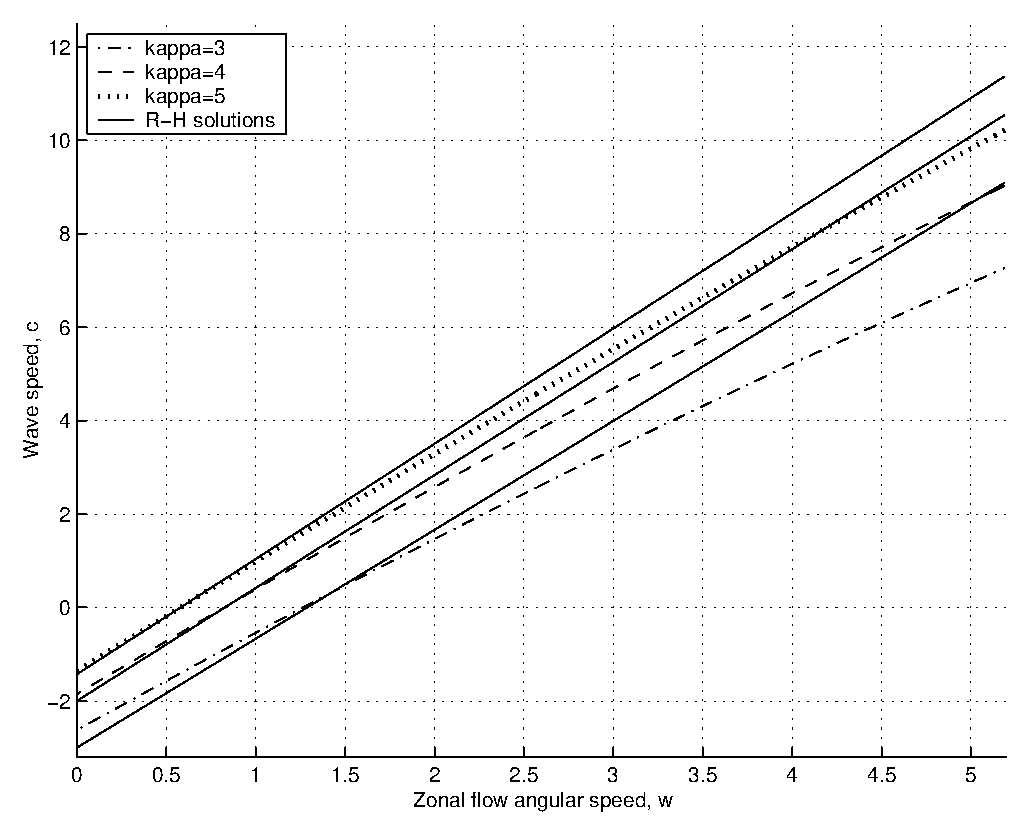
\includegraphics[scale=0.7]{IMAGES/wvchconstcomp.eps}
	\caption{Comparison of compressible linearized and Rossby--Haurwitz solutions for $\kappa=3,4$ and 5 with $N=100$.}
	\label{fig:wvccomp}
\end{figure}
To \index{Rossby--Haurwitz!comparison with compressible\\linearized solution}compare the two solution types we consider the primary physical eigenvalues for $\kappa=3,4$ and 5 with the equivalent Rossby--Haurwitz solutions over a reasonable range of allowable $\omega$ values. Figure~\ref{fig:wvccomp} shows the results of this comparison, with the solid lines representing the equivalent Rossby--Haurwitz solution for $\kappa=3$ to 5 from bottom to top respectively. In general one can conclude that the two models are in good broad agreement and we see that the behaviour of the compressible linearized solutions in not dissimilar to that of the incompressible linearized solutions, as shown in Figure~\ref{fig:wvcincomp} of Chapter~\ref{chap:2}. We also note that because the Haurwitz model has no provision for fixing the total mass $M_b$ of the atmosphere, differences are to be expected between that model and the work presented here. The discrepancies are most noticeable for larger values of the parameter $\omega$ where the effect of the mass matching condition has greater influence on the solution.

Figures~\ref{fig:swfscontscomp}--\ref{fig:swpcontscomp} present \index{polar stereographic projection}polar stereographic projections of the free-surface, density and pressure contours respectively. The scaling of the amplitude, via the linearization parameter $\epsilon$, was chosen so that the free-surface \index{height field matching}height matched the non-dimensional height of the Rossby--Haurwitz wave at $(\eta,\phi)=(0,\pi/4)$. This is similar to the technique that was used to match the incompressible and Rossby--Haurwitz solutions in Section~\ref{subsec:rhandlincomp} of Chapter~\ref{chap:2}. The scaling is arbitrary and is only used here so that visual confirmation of the general wave structure can be made.

\begin{figure}[htbp]
	\centering
		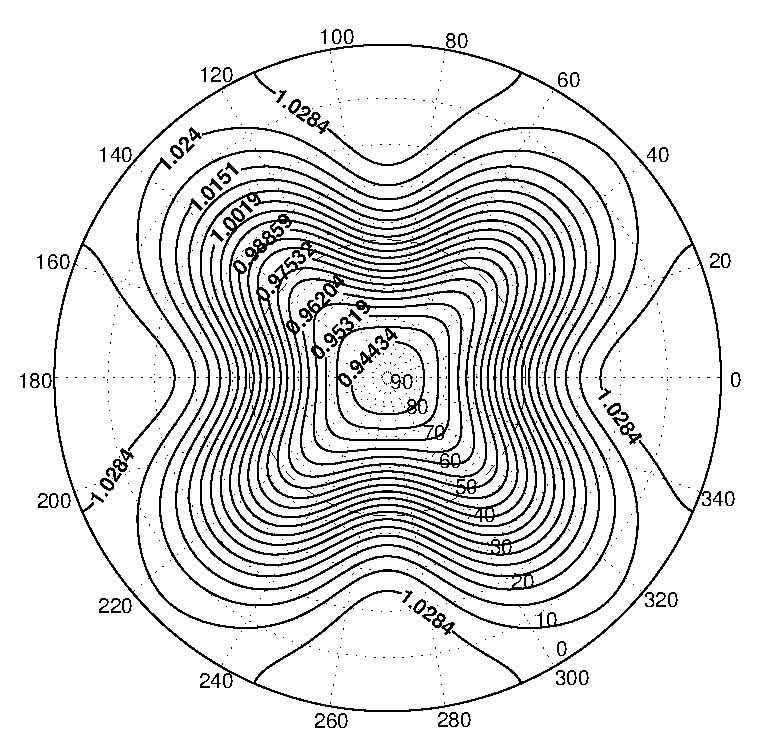
\includegraphics[scale=0.75]{IMAGES/swfscontscomp.eps}
	\caption{Compressible linearized free-surface contours for $\kappa=4$ with $N=100$.}
	\label{fig:swfscontscomp}
\end{figure}
It is evident that the compressible free-surface contours of Figure~\ref{fig:swfscontscomp} are quite similar in shape to those of the incompressible linearized theory (see Figure~\ref{fig:swfsconts}) and hence need no further comment. The density and pressure contours can be constructed once the free-surface shape is given, according to \eqref{eq:dencompnon2} and \eqref{eq:pcompnon2}. Examination of the density contours in Figure~\ref{fig:swrhocontscomp} reveals that the fluctuation in density about the mean sea-level value of $\rho=1$ is in reasonable agreement with that normally encountered in the Earth's atmosphere. Density values in Figure~\ref{fig:swrhocontscomp} range from approximately 85\% to 110\% of the mean sea-level value. Similar fluctuations are observed in the pressure field of Figure~\ref{fig:swpcontscomp}. Note also that the pressure and density contours are nearly parallel, so that the flow can be described as departing only slightly from that of \index{barotropic flow}barotropic flow.
\begin{figure}[htbp]
	\centering
		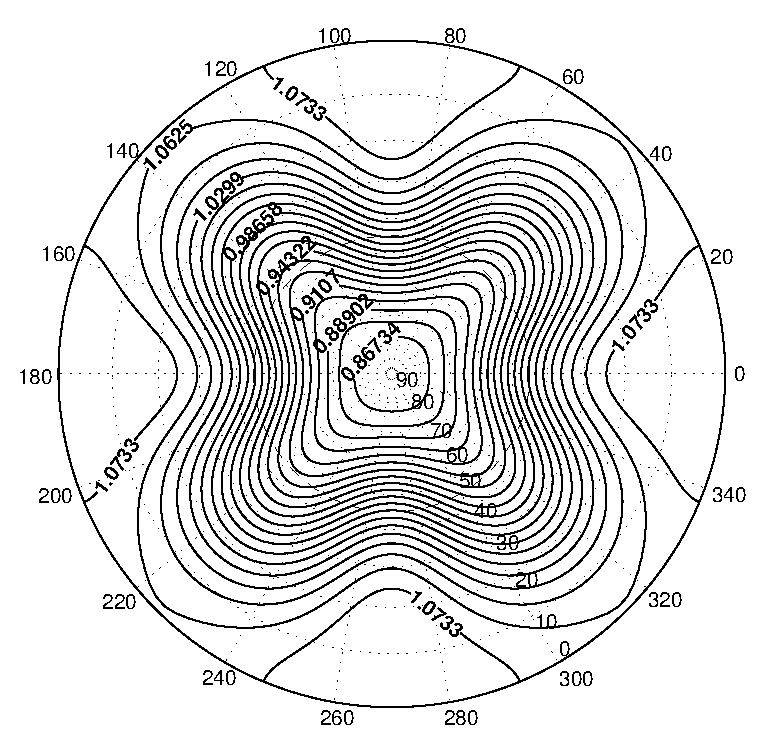
\includegraphics[scale=0.80]{IMAGES/swrhocontscomp.eps}
	\caption{Compressible linearized density contours for $\kappa=4$ with $N=100$.}
	\label{fig:swrhocontscomp}
\end{figure}

\begin{figure}[htbp]
	\centering
		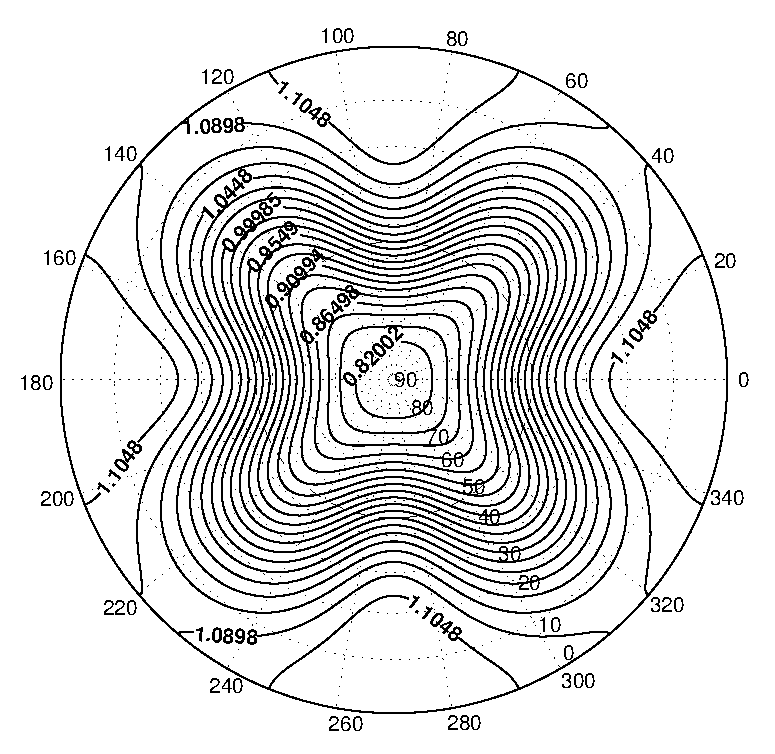
\includegraphics[scale=0.75]{IMAGES/swpcontscomp.eps}
	\caption{Compressible linearized pressure contours for $\kappa=4$ with $N=100$.}
	\label{fig:swpcontscomp}
\end{figure}

\begin{figure}[htbp]
	\centering
		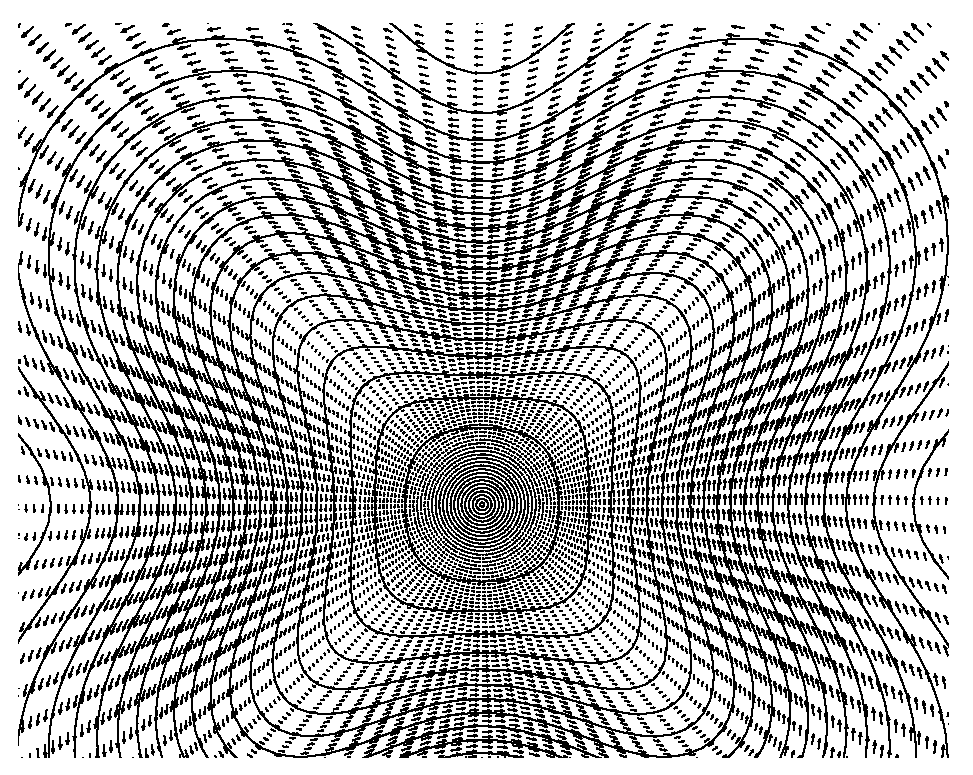
\includegraphics[scale=0.75]{IMAGES/pandvelfieldcomp.eps}
	\caption{Compressible linearized pressure contours with corresponding velocity vector field for $\kappa=4$ with $N=100$}
	\label{fig:pandvelfieldcomp}
\end{figure}

Figure~\ref{fig:pandvelfieldcomp} demonstrates the nature of the velocity vector field associated with the pressure field of Figure~\ref{fig:swpcontscomp}. The flow is observed to be predominantly \index{geostrophic approximation}geostrophic with the fluid streamlines essentially coinciding with the pressure contours.  Additionally we have increasingly diminishing flow as we approach either pole, which converges to the required stagnation point when $\phi=\pm \pi/2$.  The general nature of the fluid flow is directed in the same direction as the underlying zonal flow with the Rossby wave pattern moving relative to this mean fluid progression in an anti-clockwise manner, as expected for this particular map projection of the Northern Hemisphere.

% app0.tex (file to switch to appendix mode)
% No need to alter this file...
\appendix

% app1.tex (will be Appendix A)

\chapter[SELECTED PROOFS AND DERIVATIONS]{Selected Proofs and Derivations}

\newpage
\section{Proof of Lemma}

\noindent \textbf{Proof}:\quad The result is clearly obvious.

% app2.tex (will be Appendix B)

\chapter[COMPRESSIBLE LINEARIZED SYSTEM DERIVATION]{COMPRESSIBLE LINEARIZED SYSTEM DERIVATION}
\label{App:2}

The individual equations that comprise the rows of the linear system given by \eqref{eq:geneigen} are obtained by using orthogonality of the base expansion functions. The general process is identical to that used in section~\ref{subsec:lingalerl} of chapter~\ref{chap:2} and will not be repeated here. Rather, we simply state the results of the integrations and algebraic manipulations. For integer truncation level $N$, the truncated system of equations corresponding to conservation of mass, given by equation \eqref{eq:commasslin2}, is as follows:
for $l=1$ we have
\begin{align}
&\left[- \frac{\kappa(\gamma-1)h_o}{\gamma} -\frac{3\kappa \omega \mathrm{Fr}^2 (\gamma-1)}{8 \gamma}\left( \frac{1}{\mathrm{Ro}}+\omega \right)\right] P_{\kappa,1} -\frac{\kappa \omega \mathrm{Fr}^2(\gamma-1)}{8\gamma}\left( \frac{1}{\mathrm{Ro}}+\omega \right)P_{\kappa,2} \notag \\
&\quad+ \left[\frac{h_o(\gamma-1)}{2\gamma} +\frac{\omega \mathrm{Fr}^2(\gamma-3)}{8\gamma}\left( \frac{1}{\mathrm{Ro}}+\omega \right)\right] Q_{\kappa,1} + \frac{\omega \mathrm{Fr}^2(\gamma-3)}{16\gamma}\left( \frac{1}{\mathrm{Ro}}+\omega \right) Q_{\kappa,2} \notag \\
&\quad+\frac{3\kappa \omega}{2}H_{\kappa,1}-\frac{\kappa \omega}{2}H_{\kappa,2}=c\left[\frac{3\kappa \mathrm{Sr}}{2}H_{\kappa,1}-\frac{\kappa \mathrm{Sr}}{2}H_{\kappa,2} \right],\label{eq:commassl0}
\end{align}
for $l=2$ we have
\begin{align}
&-\frac{\kappa \omega \mathrm{Fr}^2(\gamma-1)}{8\gamma}\left( \frac{1}{\mathrm{Ro}}+\omega \right)P_{\kappa,1} + \left[-\frac{\kappa h_o(\gamma-1)}{\gamma} -\frac{\kappa \omega \mathrm{Fr}^2(\gamma-1)}{4\gamma}\left( \frac{1}{\mathrm{Ro}}+\omega \right)\right] P_{\kappa,2} \notag \\
&\,-\frac{\kappa \omega \mathrm{Fr}^2(\gamma-1)}{8\gamma}\left( \frac{1}{\mathrm{Ro}}+\omega \right)P_{\kappa,3} + \left[\frac{3 h_o(\gamma-1)}{2\gamma} +\frac{\omega \mathrm{Fr}^2(9\gamma-7)}{16\gamma}\left( \frac{1}{\mathrm{Ro}}+\omega \right)\right] Q_{\kappa,1} \notag \\
&\,+\left[\frac{3 h_o(\gamma-1)}{2\gamma} +\frac{\omega \mathrm{Fr}^2(9\gamma-11)}{16\gamma}\left( \frac{1}{\mathrm{Ro}}+\omega \right)\right] Q_{\kappa,2} +\frac{\omega \mathrm{Fr}^2(3\gamma-5)}{16\gamma}\left( \frac{1}{\mathrm{Ro}}+\omega \right) Q_{\kappa,3} \notag \\
&\,+\frac{\kappa \omega}{2}H_{\kappa,1}-\kappa \omega H_{\kappa,2}+\frac{\kappa \omega}{2}H_{\kappa,3}=c\left[\frac{\kappa \mathrm{Sr}}{2} H_{\kappa,1}-\kappa \mathrm{Sr} H_{\kappa,2}+\frac{\kappa \mathrm{Sr}}{2} H_{\kappa,3} \right], \label{eq:commassl2}
\end{align}
for $3\le l\le N-1$ we have
\begin{align}
&-\frac{\kappa \omega \mathrm{Fr}^2(\gamma-1)}{8\gamma}\left( \frac{1}{\mathrm{Ro}}+\omega \right)P_{\kappa,l-1} + \Biggl[-\frac{\kappa h_o(\gamma-1)}{\gamma} \notag \\
&\quad-\frac{\kappa \omega \mathrm{Fr}^2(\gamma-1)}{4\gamma}\left( \frac{1}{\mathrm{Ro}}+\omega \right)\Biggr] P_{\kappa,l}-\frac{\kappa \omega \mathrm{Fr}^2(\gamma-1)}{8\gamma}\left( \frac{1}{\mathrm{Ro}}+\omega \right)P_{\kappa,l+1} \notag \\
&\quad+\frac{\omega \mathrm{Fr}^2[2(l-2)(\gamma-1)+3\gamma-1]}{16\gamma}\left( \frac{1}{\mathrm{Ro}}+\omega \right)Q_{\kappa,l-2} \notag\\
&\quad+ \left[\frac{(2l-1) h_o(\gamma-1)}{2\gamma} +\frac{\omega \mathrm{Fr}^2[6(l-1)(\gamma-1)+3\gamma-1]}{16\gamma}\left( \frac{1}{\mathrm{Ro}}+\omega \right)\right] Q_{\kappa,l-1} \notag \\
&\quad+\left[\frac{(2l-1) h_o(\gamma-1)}{2\gamma}+\frac{\omega \mathrm{Fr}^2[6l(\gamma-1)-3\gamma+1]}{16\gamma}\left( \frac{1}{\mathrm{Ro}}+\omega \right)\right] Q_{\kappa,l} \notag \\
&\quad+\frac{\omega \mathrm{Fr}^2[2(l+1)(\gamma-1)-3\gamma+1]}{16\gamma}\left( \frac{1}{\mathrm{Ro}}+\omega \right) Q_{\kappa,l+1} \notag \\
&\quad+\frac{\kappa \omega (-1)^l}{2}H_{\kappa,l-1}-\kappa \omega (-1)^l H_{\kappa,l}
+\frac{\kappa \omega (-1)^l}{2}H_{\kappa,l+1} \notag \\
&\quad=c\left[\frac{\kappa \mathrm{Sr}(-1)^l}{2} H_{\kappa,l-1}-\kappa \mathrm{Sr}(-1)^l H_{\kappa,l}+\frac{\kappa \mathrm{Sr}(-1)^l}{2} H_{\kappa,l+1} \right] \label{eq:commassl3p}
\end{align}
and for $l=N$ we have
\begin{align}
&-\frac{\kappa \omega \mathrm{Fr}^2(\gamma-1)}{8\gamma}\left( \frac{1}{\mathrm{Ro}}+\omega \right)P_{\kappa,N-1} + \Biggl[-\frac{\kappa h_o(\gamma-1)}{\gamma} \notag \\
&\quad-\frac{\kappa \omega \mathrm{Fr}^2(\gamma-1)}{4\gamma}\left( \frac{1}{\mathrm{Ro}}+\omega \right)\Biggr] P_{\kappa,N} \notag \\
&\quad+\frac{\omega \mathrm{Fr}^2[2(N-2)(\gamma-1)+3\gamma-1]}{16\gamma}\left( \frac{1}{\mathrm{Ro}}+\omega \right)Q_{\kappa,N-2} \notag\\
&\quad+ \left[\frac{(2N-1) h_o(\gamma-1)}{2\gamma} +\frac{\omega \mathrm{Fr}^2[6(N-1)(\gamma-1)+3\gamma-1]}{16\gamma}\left( \frac{1}{\mathrm{Ro}}+\omega \right)\right] Q_{\kappa,N-1} \notag \\
&\quad+\left[\frac{(2N-1) h_o(\gamma-1)}{2\gamma}+\frac{\omega \mathrm{Fr}^2[6N(\gamma-1)-3\gamma+1]}{16\gamma}\left( \frac{1}{\mathrm{Ro}}+\omega \right)\right] Q_{\kappa,N} \notag \\
&\quad+\frac{\kappa \omega (-1)^N}{2}H_{\kappa,N-1}-\kappa \omega (-1)^N H_{\kappa,N}
 =c\left[\frac{\kappa \mathrm{Sr}(-1)^N}{2} H_{\kappa,N-1}-\kappa \mathrm{Sr}(-1)^N H_{\kappa,N} \right] \label{eq:commasslN}
\end{align}

For the $\lambda$-momentum equation given by \eqref{eq:comlamlin2}, the individual component equations of the linear system are given by: for $l=0$,
\begin{equation}
-\frac{\kappa \omega}{2} P_{\kappa,1}-\frac{1}{4}\left(\frac{1}{\mathrm{Ro}}+\omega \right) Q_{\kappa,1} + \frac{\kappa}{\mathrm{Fr}^2} H_{\kappa,1} = c\left[-\frac{\kappa \mathrm{Sr}}{2} P_{\kappa,1} \right], \label{eq:comlaml0}
\end{equation}
for $l=1$,
\begin{multline}
-\frac{\kappa \omega}{2} P_{\kappa,1}-\frac{\kappa \omega}{2} P_{\kappa,2}-\frac{1}{4}\left(\frac{1}{\mathrm{Ro}}+\omega \right) Q_{\kappa,2} + \frac{\kappa}{\mathrm{Fr}^2} H_{\kappa,1}- \frac{\kappa}{\mathrm{Fr}^2} H_{\kappa,2} \\
= c\left[-\frac{\kappa \mathrm{Sr}}{2} P_{\kappa,1} -\frac{\kappa \mathrm{Sr}}{2} P_{\kappa,2}\right] \label{eq:comlaml1}
\end{multline}
and for $l\ge2$,
\begin{multline}
-\frac{\kappa \omega}{2} P_{\kappa,l}-\frac{\kappa \omega}{2} P_{\kappa,l+1}+\frac{1}{4}\left(\frac{1}{\mathrm{Ro}}+\omega \right) Q_{\kappa,l-1}-\frac{1}{4}\left(\frac{1}{\mathrm{Ro}}+\omega \right) Q_{\kappa,l+1} \\- \frac{\kappa(-1)^l}{\mathrm{Fr}^2} H_{\kappa,l}+ \frac{\kappa(-1)^l}{\mathrm{Fr}^2} H_{\kappa,l+1}
= c\left[-\frac{\kappa \mathrm{Sr}}{2} P_{\kappa,l} -\frac{\kappa \mathrm{Sr}}{2} P_{\kappa,l+1}\right]. \label{eq:comlaml2p}
\end{multline}

Similarly, from the $\phi$ momentum equation \eqref{eq:comphilin2} we have: for $1\le l \le N-1$,
\begin{multline}
\frac{1}{2}\left(\frac{1}{\mathrm{Ro}}+\omega \right)P_{\kappa,l}-\frac{1}{2}\left(\frac{1}{\mathrm{Ro}}+\omega \right)P_{\kappa,l+1}+\kappa \omega Q_{\kappa,l} + \frac{2l(-1)^{l+1}}{\mathrm{Fr}^2} H_{\kappa,l}\\- \frac{2l(-1)^{l+1}}{\mathrm{Fr}^2} H_{\kappa,l+1}=c\left[\kappa \mathrm{Sr} Q_{\kappa,l}\right], \label{eq:comphil1p}
\end{multline}
and for $l=N$ we have
\begin{equation}
\frac{1}{2}\left(\frac{1}{\mathrm{Ro}}+\omega \right)P_{\kappa,N}+\kappa \omega Q_{\kappa,N} + \frac{2N(-1)^{N+1}}{\mathrm{Fr}^2} H_{\kappa,N}=c\left[\kappa \mathrm{Sr} Q_{\kappa,N}\right]. \label{eq:comphilN}
\end{equation}
These relations are then used to construct the generalized eigenvalue problem expressed by \eqref{eq:geneigen}.
% Add in the bibliography
% Set the text size to be small
\small
% Set the bibliography style to be plain.
\bibliographystyle{plain}
% List all citations in thesis.bib file
% Comment this out for final printing
% if you have un-cited items in your
% bib database
\nocite{*}
% thesis.bib is the name of our database
% and we load it with the following command
\bibliography{thesis}

% A small file that prints the index in the main document.
% No need to alter this file...
\printindex


\end{document}
